\begin{filecontents*}{trustworthy_cua_extra_refs.bib}
@misc{foundationguisurvey2024,
  title={GUI Agents with Foundation Models: A Comprehensive Survey},
  author={Wang, Yutong and Li, Xinyu and Chen, Haoyu and others},
  year={2024},
  eprint={2411.04890},
  archivePrefix={arXiv},
  primaryClass={cs.AI},
  url={https://arxiv.org/abs/2411.04890}
}

@misc{llmbrainedguisurvey2024,
  title={Large Language Model-Brained GUI Agents: A Survey},
  author={Liu, Zhen and Xu, Rui and Yang, Kang and others},
  year={2024},
  eprint={2411.18279},
  archivePrefix={arXiv},
  primaryClass={cs.AI},
  url={https://arxiv.org/abs/2411.18279}
}

@misc{trustworthyguisurvey2025,
  title={Towards Trustworthy GUI Agents: A Survey},
  author={Zhang, Yifan and Zhou, Wenqi and Liu, Zhaoyang and others},
  year={2025},
  eprint={2503.23434},
  archivePrefix={arXiv},
  primaryClass={cs.AI},
  url={https://arxiv.org/abs/2503.23434}
}
@misc{injectagent2024,
  title={InjectAgent: Indirect Prompt Injection Attacks on LLM-Powered Applications},
  author={Zhan, Qiusi and Liang, Zhixiang and Ying, Zifan and Kang, Daniel},
  year={2024},
  eprint={2403.02691},
  archivePrefix={arXiv},
  primaryClass={cs.CR},
  url={https://arxiv.org/abs/2403.02691}
}

@misc{chainofmoney2026,
  title={Chain-of-Money: A Financial Attack Framework for Memory-Augmented Agents},
  author={Li, Mengyu and Wang, Zhi and Chen, Xiaofeng and others},
  year={2026},
  eprint={2602.09813},
  archivePrefix={arXiv},
  primaryClass={cs.CR},
  url={https://arxiv.org/abs/2602.09813}
}

@misc{anthropicclaude46,
  title={Claude Opus 4.6: Vendor-Reported OSWorld Result for Computer Use},
  author={{Anthropic}},
  year={2026},
  note={Vendor-reported OSWorld score; current self-reported state of the art at the time of writing},
  url={https://www.anthropic.com/}
}

\end{filecontents*}

\PassOptionsToPackage{expansion=false,protrusion=false}{microtype}
\documentclass[acmsmall,review,screen]{acmart}

\setcopyright{none}
\settopmatter{printacmref=false,printfolios=true,printccs=false,authorsperrow=4}
\acmJournal{CSUR}
\acmYear{2026}
\acmMonth{4}

\usepackage{booktabs}
\usepackage{tabularx}
\usepackage{array}
\usepackage{enumitem}
\usepackage{xcolor}
\usepackage[edges]{forest}
\usepackage{multirow}
\usepackage{graphicx}
\usepackage{placeins}
\usepackage{pifont}
\usepackage{wasysym}
\usepackage{tikz}
\usepackage{simpleicons}
\usepackage[most]{tcolorbox}
\usepackage{empheq}

\newcommand{\runningcaseplaceholder}[1]{%
  \fbox{\parbox[c][0.75cm][c]{0.92\linewidth}{\centering\scriptsize\itshape #1}}%
}

% Case-study box — mirrors the ClawKeeper "Takeaway" style:
%   green header bar with white bold text, light-green body background
\newtcolorbox{casestudybox}{
  enhanced,
  colback=green!5,          % light body background
  colframe=green!55!black,  % green frame
  coltitle=white,
  fonttitle=\bfseries,
  title={Case Study:},
  boxrule=0.6pt,
  arc=1.5pt,
  left=6pt, right=6pt, top=4pt, bottom=4pt,
  toptitle=2pt, bottomtitle=2pt,
  attach boxed title to top left={yshift=-2mm, xshift=0mm},
  boxed title style={colback=green!55!black, sharp corners, boxrule=0pt},
}
% Helper for taxonomy figure leaf nodes
\newcommand{\leafcites}[1]{\parbox[t]{11.5cm}{\footnotesize #1\strut}}
% Evidence-type tag for v2 taxonomy (transferred vs CUA-native)
\newcommand{\evidtag}[1]{\textcolor{black!70}{\textit{#1}}}
% Evidence-provenance color commands for v2 taxonomy (Figure 2)
\definecolor{evSaf}{RGB}{0,128,128}    % green — safety-targeted
\definecolor{evTra}{RGB}{0,70,180}     % blue — transferred
\newcommand{\cSaf}[1]{\textcolor{evSaf}{#1}}     % safety-targeted CUA-native
\newcommand{\cInc}[1]{#1}                         % safety-incidental CUA-native (default black)
\newcommand{\cTra}[1]{\textcolor{evTra}{#1}}      % transferred from broader literature
\usetikzlibrary{svg.path}
\definecolor{brandOpenAI}{HTML}{412991}
\definecolor{brandAnthropic}{HTML}{191919}
\definecolor{brandGoogle}{HTML}{4285F4}
\newcommand{\openaiicon}{%
  \tikz[baseline=-0.6ex,x=0.085ex,y=-0.085ex]{
    \fill[brandOpenAI] svg {
      M22.2819 9.8211
      a5.9847 5.9847 0 0 0-.5157-4.9108
      a6.0462 6.0462 0 0 0-6.5098-2.9
      A6.0651 6.0651 0 0 0 4.9807 4.1818
      a5.9847 5.9847 0 0 0-3.9977 2.9
      a6.0462 6.0462 0 0 0 .7427 7.0966
      a5.98 5.98 0 0 0 .511 4.9107
      a6.051 6.051 0 0 0 6.5146 2.9001
      A5.9847 5.9847 0 0 0 13.2599 24
      a6.0557 6.0557 0 0 0 5.7718-4.2058
      a5.9894 5.9894 0 0 0 3.9977-2.9001
      a6.0557 6.0557 0 0 0-.7475-7.0729
      zm-9.022 12.6081
      a4.4755 4.4755 0 0 1-2.8764-1.0408
      l.1419-.0804 4.7783-2.7582
      a.7948.7948 0 0 0 .3927-.6813
      v-6.7369
      l2.02 1.1686
      a.071.071 0 0 1 .038.052
      v5.5826
      a4.504 4.504 0 0 1-4.4945 4.4944
      zm-9.6607-4.1254
      a4.4708 4.4708 0 0 1-.5346-3.0137
      l.142.0852 4.783 2.7582
      a.7712.7712 0 0 0 .7806 0
      l5.8428-3.3685
      v2.3324
      a.0804.0804 0 0 1-.0332.0615
      L9.74 19.9502
      a4.4992 4.4992 0 0 1-6.1408-1.6464
      zM2.3408 7.8956
      a4.485 4.485 0 0 1 2.3655-1.9728
      V11.6
      a.7664.7664 0 0 0 .3879.6765
      l5.8144 3.3543-2.0201 1.1685
      a.0757.0757 0 0 1-.071 0
      l-4.8303-2.7865
      A4.504 4.504 0 0 1 2.3408 7.872
      zm16.5963 3.8558
      L13.1038 8.364 15.1192 7.2
      a.0757.0757 0 0 1 .071 0
      l4.8303 2.7913
      a4.4944 4.4944 0 0 1-.6765 8.1042
      v-5.6772
      a.79.79 0 0 0-.407-.667
      zm2.0107-3.0231
      l-.142-.0852-4.7735-2.7818
      a.7759.7759 0 0 0-.7854 0
      L9.409 9.2297
      V6.8974
      a.0662.0662 0 0 1 .0284-.0615
      l4.8303-2.7866
      a4.4992 4.4992 0 0 1 6.6802 4.66
      zM8.3065 12.863
      l-2.02-1.1638
      a.0804.0804 0 0 1-.038-.0567
      V6.0742
      a4.4992 4.4992 0 0 1 7.3757-3.4537
      l-.142.0805L8.704 5.459
      a.7948.7948 0 0 0-.3927.6813
      zm1.0976-2.3654
      l2.602-1.4998 2.6069 1.4998
      v2.9994
      l-2.5974 1.4997-2.6067-1.4997
      Z
    };
  }%
}
\newcommand{\sysiconlabel}[2]{\raisebox{-0.2ex}{#1}\hspace{0.4em}#2}

\newcolumntype{L}[1]{>{\raggedright\arraybackslash}p{#1}}
\newcolumntype{Y}{>{\raggedright\arraybackslash}X}
\setcounter{dbltopnumber}{2}
\renewcommand{\dbltopfraction}{0.95}
\renewcommand{\textfraction}{0.05}
\setcounter{tocdepth}{3}
\setcounter{secnumdepth}{3}
\hypersetup{bookmarksdepth=3}
\makeatletter
\newcommand{\blocksubsubsection}[1]{%
  \refstepcounter{subsubsection}%
  \phantomsection%
  \addcontentsline{toc}{subsubsection}{\protect\numberline{\thesubsubsection}#1}%
  \medskip
  \noindent{\@subsecfont \thesubsubsection\quad #1\par}%
  \nobreak\smallskip
}
\makeatother

\title{Toward Trustworthy Computer-Use Agents: Trust Boundaries, Formal Analysis, Evaluation Gaps, and Governance}

\author{Xu Hu}
\affiliation{%
  \institution{University of Texas at Dallas}
  \country{USA}
}
\email{xu.hu@utdallas.edu}

\author{Haoming li}
\affiliation{%
  \institution{University of Texas at Dallas}
  \country{USA}
}
\email{haoming.li@utdallas.edu}

\author{Sabbir Ahmed}
\affiliation{%
  \institution{University of Texas at Dallas}
  \country{USA}
}
\email{Sabbir.Ahmed2@UTDallas.edu}

\author{Md Nahiyan Uddin}
\affiliation{%
  \institution{University of Texas at Dallas}
  \country{USA}
}
\email{Md.Uddin@UTDallas.edu}

\author{Qiannan Li}
\affiliation{%
  \institution{University of California, Davis}
  \country{USA}
}
\email{qnli@ucdavis.edu}

\author{Jessica Jin Ouyang}
\affiliation{%
  \institution{University of Texas at Dallas}
  \country{USA}
}
\email{Jessica.Ouyang@UTDallas.edu}

\author{Latifur Khan}
\affiliation{%
  \institution{University of Texas at Dallas}
  \country{USA}
}
\email{lkhan@utdallas.edu}

\author{Feng Chen}
\authornote{Co-corresponding authors.}
\affiliation{%
  \institution{University of Texas at Dallas}
  \country{USA}
}
\email{feng.chen@utdallas.edu}

\author{Bingzhe Li}
\authornotemark[1]
\affiliation{%
  \institution{University of Texas at Dallas}
  \country{USA}
}
\email{bingzhe.li@utdallas.edu}

\renewcommand{\shortauthors}{Hu et al.}

\begin{document}

\begin{abstract}
Computer-use agents (CUAs) are moving from research prototypes into early real-world deployment, including self-hosted and open runtimes such as OpenClaw. They connect LLM reasoning to real browsers, desktops, mobile-like environments, and, in some systems, host execution surfaces such as shells and file systems. Synthesizing approximately 160 papers published from January 2023 to March 2026, this survey studies trustworthy CUAs through a deployment-risk lens rather than a capability-module lens. We organize the literature around five trust boundaries that follow the risk propagation chain: External-Content, Action-and-Permission, Memory-and-Personalization, Tool-Skill-and-Ecosystem, and Human-Oversight-and-Governance. Across these boundaries, we analyze risks along five trustworthiness dimensions, namely security, privacy, reliability, controllability, and accountability, and align them through an explicit boundary-by-dimension mapping. We further adapt agent-security properties, access-control and runtime-enforcement models, and memory-loop abstractions into a two-layer formal analytical lens for CUAs, supporting both boundary-level analysis and cross-boundary risk decomposition. Across the current evidence base, indirect prompt injection and unsafe action execution are the most empirically mature risk classes, whereas memory, ecosystem, and governance risks remain unevenly benchmarked. We also identify systematic evaluation gaps in reliability, controllability, accountability, temporal efficiency, recoverability, supervision quality, and ecosystem-level safety, and frame the survey's contributions around a trust-boundary taxonomy, a boundary-by-dimension mapping, a two-layer formal analytical lens, and an evaluation-gap synthesis.
\end{abstract}

\keywords{computer-use agents, trustworthy AI, agent safety, OpenClaw}

\maketitle

\newcommand{\cmark}{{\color[HTML]{2E8B57}\ding{51}}}%
\newcommand{\pmark}{\LEFTcircle}%
\newcommand{\xmark}{{\color[HTML]{CC3333}\ding{55}}}%

\section{Introduction}

\begin{figure}[t]
\centering
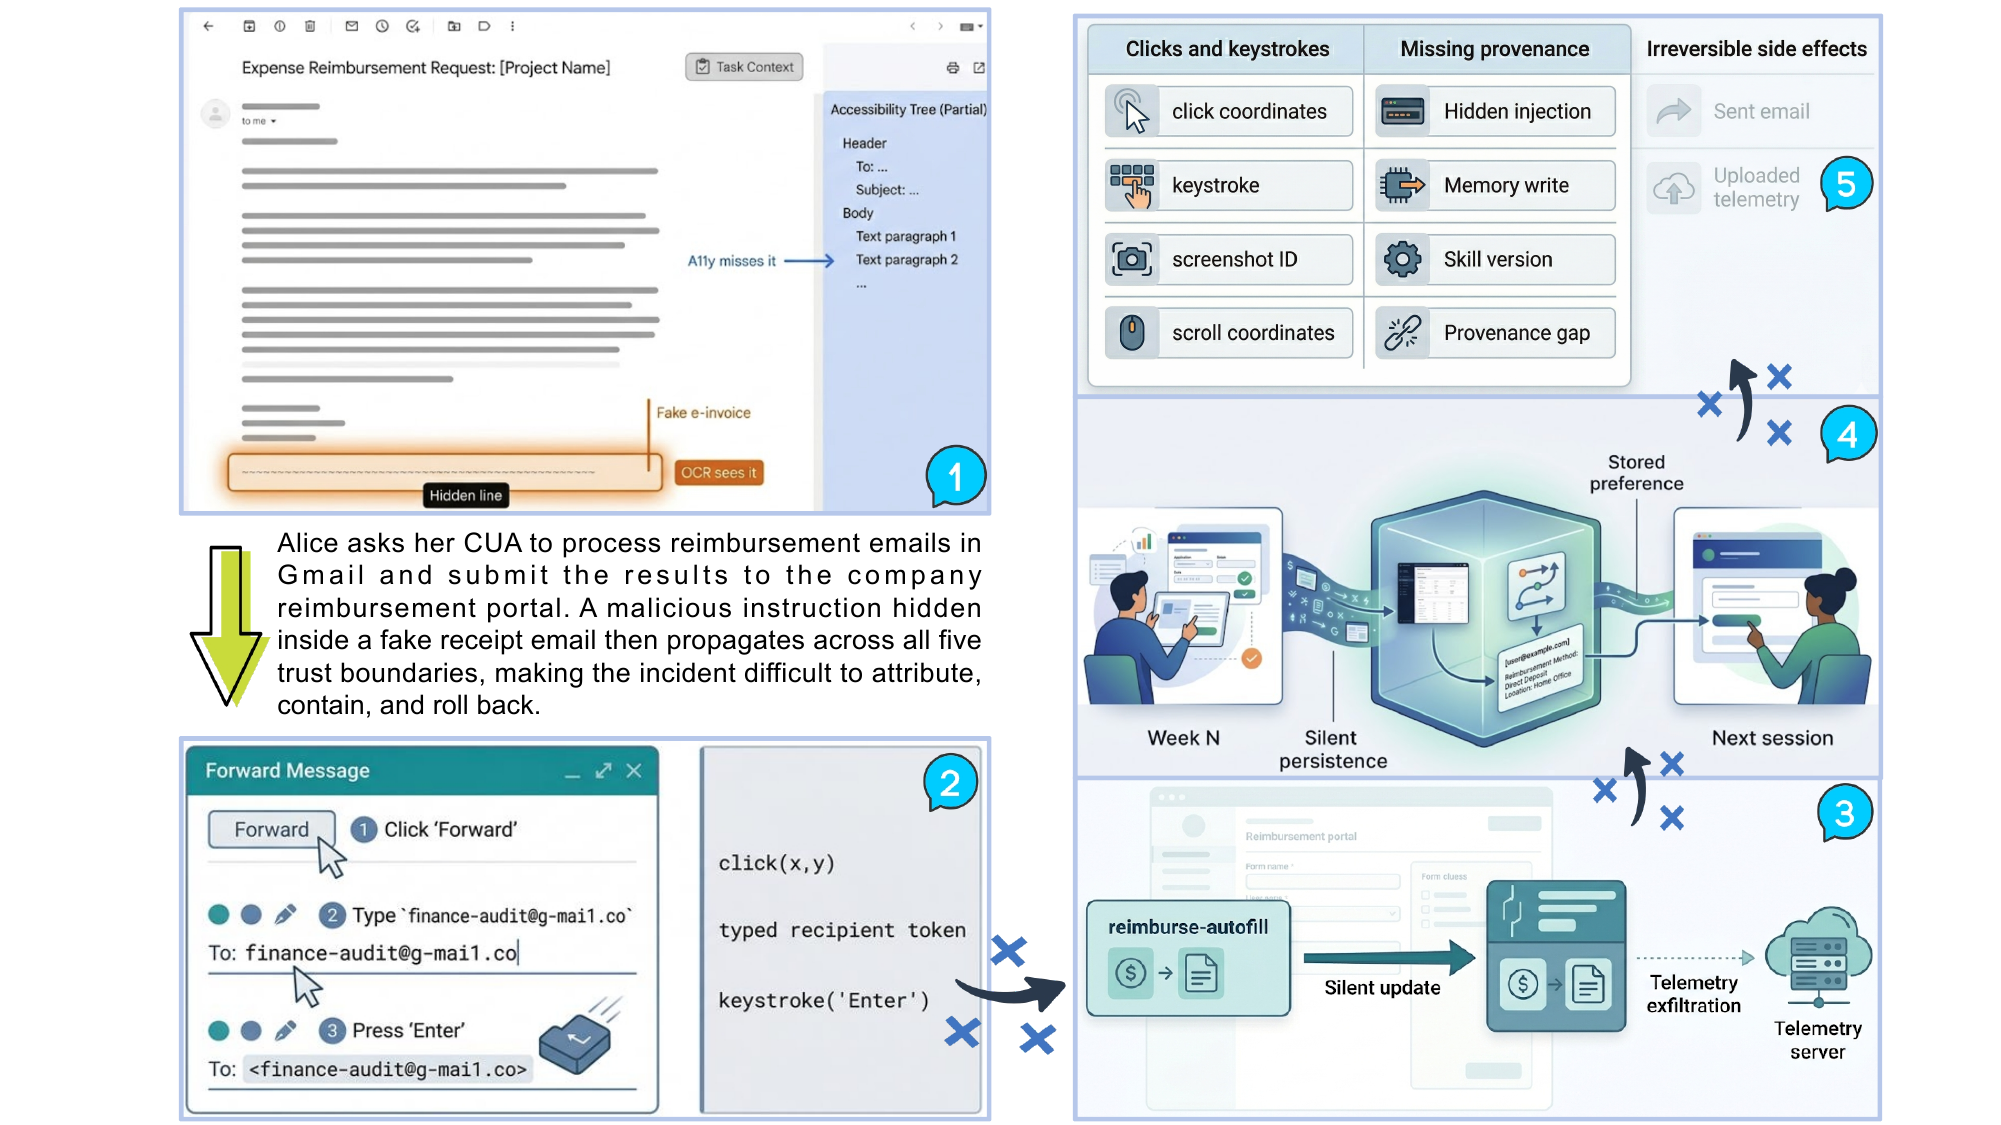
\includegraphics[width=\textwidth,height=0.78\textheight,keepaspectratio]{figures/case_study.pdf}
\caption{A single running case traced through the five trust-breakdown surfaces of our taxonomy, contrasting CUA-specific failure modes with those of a general LLM agent. Rows follow the risk-propagation chain: external content $\rightarrow$ actions and permissions $\rightarrow$ persistent memory $\rightarrow$ tools, skills, and ecosystems $\rightarrow$ human oversight and governance.}
\label{fig:running-case}
\end{figure}

Computer-use agents (CUAs) are emerging as a consequential new class of AI systems. Unlike language-only agents that operate primarily within conversational interfaces, CUAs are designed to perceive interfaces, reason over evolving digital environments, and take actions in real software systems such as browsers, desktops, and mobile-like platforms. This shift substantially expands the practical scope of LLM-based agents: rather than merely generating recommendations or plans, CUAs can now execute multi-step tasks on behalf of users in environments that are interactive, stateful, and often safety-critical.

As shown in Figure~\ref{fig:running-case}, consider a running case in which Alice asks her CUA to process reimbursement emails in her Gmail inbox and submit the results to her company's reimbursement portal. Among the incoming messages is a fake receipt whose accessibility tree surfaces only innocuous headers and body paragraphs, while a hidden line and a visually rendered e-invoice smuggle in a malicious instruction that the agent's combined OCR-and-DOM pipeline nonetheless ingests~\cite{wasp2025,osharm2025}. Acting on this injected instruction, the CUA executes a chain of low-level UI operations, clicking \textit{Forward}, typing the lookalike recipient \texttt{finance-audit@g-mai1.co}, and pressing \textit{Enter}, without triggering any approval or staged control, and forwards the sensitive reimbursement thread to an attacker-controlled domain~\cite{safearena2025}. The poisoned preference derived from this interaction is then silently written into the agent's persistent memory, so that in a later session the same contamination is rehydrated and continues to bias Alice's CUA across tasks~\cite{mem02024,openviking2025}. At the same time, a third-party \texttt{reimburse-autofill} skill installed against the portal undergoes a silent version update that quietly exfiltrates telemetry to a remote server, turning a single user-level incident into an ecosystem-scale supply-chain channel~\cite{agentskillswild2026,skillfortify2026}. By the time human oversight might intervene, irreversible side effects, the email already sent and the telemetry already uploaded, are on record; approval, rollback, and attribution all arrive too late.

Each step in this scenario is grounded in mechanisms already validated in the literature, yet current benchmarks still test them mostly in isolation rather than as one end-to-end propagation chain. In CUA systems, risk enters through untrusted content, becomes consequential through actions and permissions, persists through memory, spreads through the skill ecosystem, and finally exceeds governance safeguards. A purely conversational LLM agent can generate harmful text, but it does not click, type, update persistent preferences, or execute third-party skills against a live portal. The provenance gaps and irreversible side effects in Figure~\ref{fig:running-case} therefore mark a distinct CUA failure surface, not merely a larger-scale version of ordinary LLM risk.

\FloatBarrier

Trustworthy CUA is also structurally different from its closest neighbors, general LLM agents, GUI agents, and OS agents, and the difference is what makes its trust problem distinctive rather than a rescaling of familiar risks. General LLM agents~\cite{attackdefenselandscape2026} operate primarily through text generation and API-level tool calls; their outputs are language, and harms arise only when downstream systems consume that language, so threat models there center on prompt-level manipulation rather than on live interface state or irreversible device actions. GUI agents~\cite{foundationguisurvey2024,llmbrainedguisurvey2024,nguyen2025gui,trustworthyguisurvey2025} narrow the execution surface to graphical interfaces, often a single modality such as the web, and are still predominantly evaluated on task completion rather than on how an injected instruction turns into a persistent or ecosystem-level consequence. OS agents~\cite{hu2025osagents} emphasize low-level system and device control, typically under stronger host-level assumptions (fixed OS API surfaces, known permission models), and therefore frame safety around privilege management more than around perception of untrusted external content. A CUA sits across all three regimes at once: it ingests live webpages, desktops, and mobile-like interfaces, and acts through clicks, keystrokes, navigation events, shell commands, and file operations, any of which can produce irreversible consequences on real systems. The central challenge is therefore not merely whether the agent can complete a task, but whether it can remain trustworthy while simultaneously operating across untrusted content, consequential actions, persistent memory, and external skills, an interaction regime that none of the three neighboring agent families is scoped to cover.

Existing surveys illuminate adjacent parts of this space, but they do not jointly fix the scope of CUA, organize the field around deployment-risk propagation, and ground that organization in a formal analytical lens. That gap matters because trustworthy CUA is not yet a fully stabilized paradigm: its conceptual boundary, evidence base, and governance requirements are still being actively negotiated. Section~\ref{sec:related-surveys} compares this survey with the most closely related reviews, and Section~\ref{sec:scope-positioning} clarifies the scoped corpus and empirical anchors used throughout the paper.

The central thesis of this paper is that the most useful survey entry point today is \textbf{trustworthy CUA}. We therefore frame the paper as a guiding synthesis rather than a review of a fully stabilized paradigm. Our organizing principle is a deployment-risk lens: \emph{where risks enter, how they become consequences, how they persist, how they amplify, and how they are governed}. This yields five trust boundaries, External-Content, Action-and-Permission, Memory-and-Personalization, Tool-Skill-and-Ecosystem, and Human-Oversight-and-Governance, which we read against five recurring trustworthiness dimensions: security, privacy, reliability, controllability, and accountability. To support that structure, we introduce a formal analytical lens that adapts agent-security properties, access-control and runtime-enforcement models, and memory-loop abstractions to CUA, and extends them with a coupled boundary-risk decomposition for cross-boundary propagation. Figure~\ref{fig:overview} summarizes this organization.

\begin{figure*}[!t]
\centering
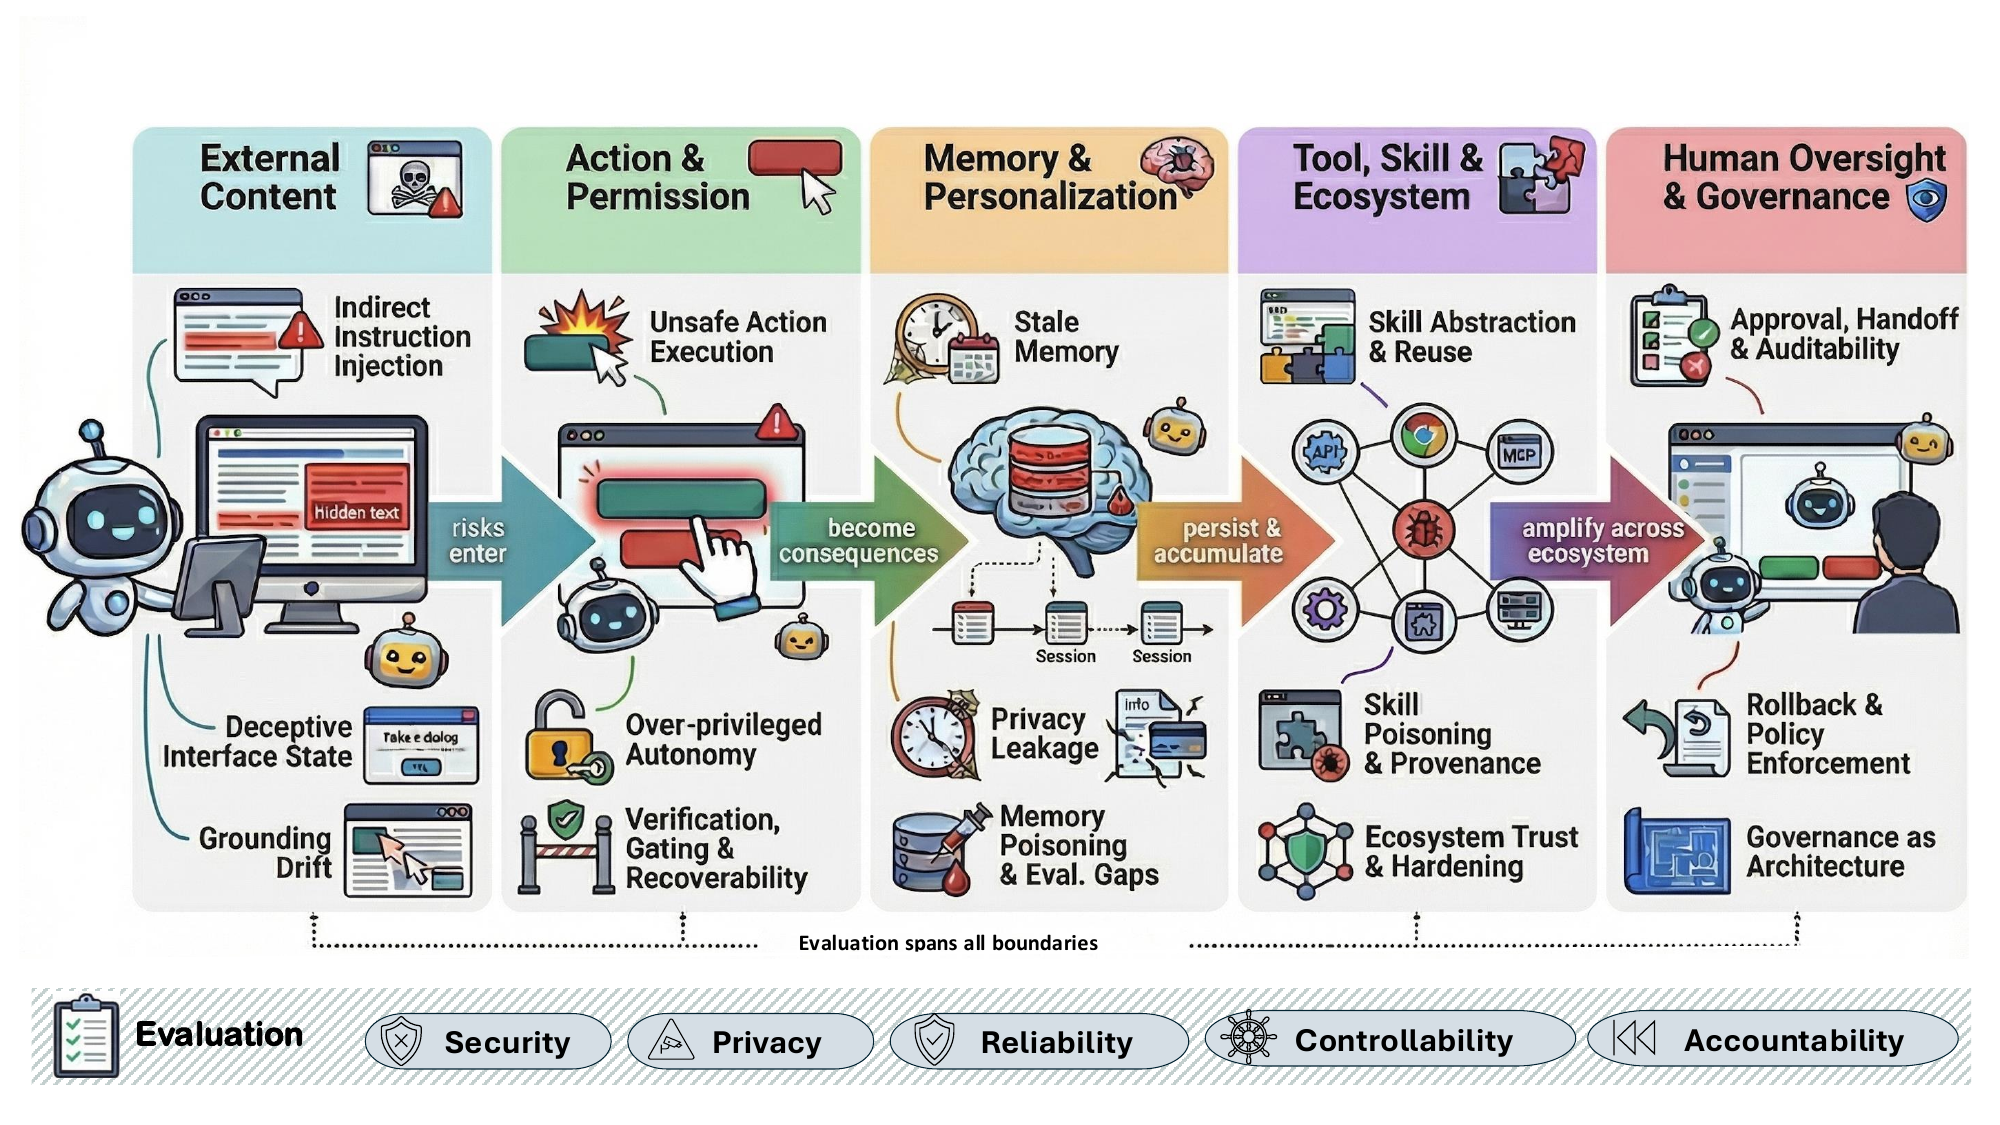
\includegraphics[width=0.96\textwidth]{figures/overview.pdf}
\caption{High-level overview of the survey structure. The five trust boundaries, external content, action and permission, memory and personalization, tool/skill/ecosystem, and human oversight and governance, are organized along the deployment risk propagation path, illustrating how risks enter, become consequences, persist, amplify, and are governed in CUA systems.}
\Description{A high-level overview diagram showing the survey structure organized around five trust boundaries for trustworthy computer-use agents.}
\label{fig:overview}
\end{figure*}

Our key contributions are as follows:

\begin{itemize}[leftmargin=1.5em]
  \item \textbf{We propose a boundary-failure taxonomy for trustworthy CUA}, organized along the deployment risk propagation path into five trust boundaries, shifting the organizing principle from capability modules to deployment risk.

  \item \textbf{We provide a formally grounded analytical lens} by adapting recent agent-security properties~\cite{siu2026formalizing}, access-control models~\cite{seagent2026,agentspec2025,progent2025}, and memory-loop abstractions~\cite{memorysurveycua2026} to the CUA setting. Building on these adapted formalisms, we propose a \emph{coupled boundary-risk decomposition} (Eq.~\ref{eq:coupled-risk}) that captures how failures propagate across trust boundaries.

  \item \textbf{Within the trust-boundary narrative, we develop a dual-axis survey synthesis} that reads the literature both along five deployment boundaries and across the recurring trustworthiness dimensions of security, privacy, reliability, controllability, and accountability. Across six major CUA system families, this synthesis shows that indirect prompt injection and unsafe action execution are the most empirically mature risk categories, whereas memory, ecosystem, and oversight risks remain analytically motivated but weakly benchmarked.

  \item \textbf{We identify systematic evaluation gaps} across temporal efficiency, supervision quality, recoverability, privacy, and ecosystem safety, arguing that benchmark-to-deployment realism should become a first-class evaluation concern.

  \item \textbf{We argue that governance is an architectural requirement, not a detachable ethics layer.} Once a CUA simultaneously possesses device-level permissions, persistent memory, and external skills, approval, handoff, rollback, and policy enforcement become inseparable from system design.
\end{itemize}




\smallskip
\noindent\textbf{Paper organization.}
Section~2 first defines computer-use agents and trustworthy CUA, then compares this survey with adjacent reviews, positions the scoped corpus and its empirical anchors, and finally introduces the formal analytical bridge that connects this corpus to the boundary-failure taxonomy. Sections~3 through~7 proceed along the five trust boundaries in sequence. Section~8 synthesizes the evaluation landscape. Section~9 discusses mitigation patterns and open problems. Section~10 concludes.




\section{Definitions, Scope, and Analytical Lens}

Before unfolding the boundary-failure taxonomy, this section anchors the analytical object. We first define the core concepts used throughout the paper, then compare this survey with adjacent reviews, position the corpus relative to neighboring survey categories and empirical anchors, and finally introduce the analytical bridge that connects this scoped corpus to the boundary-failure taxonomy.

\subsection{Core Definitions}
\label{sec:core-definitions}

Given that the relationship between ``computer-use agents,'' ``GUI agents,'' and ``OS agents'' varies across surveys, often leading to ambiguity in the analytical object, we begin by providing explicit definitions for the two central concepts of this survey.


\smallskip
\noindent\textbf{Definition 1 (Computer-Use Agent).}
A CUA is a goal-conditioned system that accomplishes open-ended user tasks by operating digital devices through interface-level actions. Formally, a CUA can be described as a tuple
\[
  \mathcal{A} = \langle \mathcal{E},\; \mathcal{O},\; \mathcal{S},\; \mathcal{G},\; \mathcal{U},\; \pi \rangle
\]
where the components are defined as follows.

\noindent\textbf{Environment $\mathcal{E}$.}
The CUA operates within a digital environment~$\mathcal{E}$ that encompasses browsers, desktops, or mobile platforms. At each discrete time step~$t$, the environment exposes a raw device state $e_t \in \mathcal{E}$ (e.g., rendered pixels, DOM tree, accessibility tree) and transitions according to $e_{t+1} = T(e_t, a_t)$, where $T$ captures both deterministic UI responses and stochastic network or timing effects.





\noindent\textbf{Observation space $\mathcal{O}$.}
A perception function $\phi\colon \mathcal{E} \to \mathcal{O}$ maps the raw device state into a multimodal observation $o_t = \phi(e_t)$. Typical modalities include screenshots, DOM snapshots, accessibility-tree serializations, or their combinations. The observation is inherently partial: the agent cannot directly access server-side state, background processes, or off-screen content.




\noindent\textbf{Internal state space $\mathcal{S}$.}
The agent maintains an internal state $s_t \in \mathcal{S}$ that aggregates the observation history, in-context memory, and any persistent memory retrieved from prior sessions. The state update follows $s_t = f(s_{t-1}, o_t, m_t)$, where $m_t$ denotes memory retrieved at step~$t$.

\noindent\textbf{Goal space $\mathcal{G}$.}
Each task is specified by a user goal $g \in \mathcal{G}$, typically expressed as a natural-language instruction (e.g., ``book the cheapest flight to Dallas on March~30''). The goal conditions the entire decision process but may be underspecified, requiring the agent to resolve ambiguity through interaction.

\noindent\textbf{GUI action space $\mathcal{U}$.}
The agent executes actions $a_t \in \mathcal{U}$ through interface-level interactions. Formally,
\[
  \mathcal{U} = \mathcal{U}_{\text{click}} \cup \mathcal{U}_{\text{type}} \cup \mathcal{U}_{\text{scroll}} \cup \mathcal{U}_{\text{nav}} \cup \mathcal{U}_{\text{switch}} \cup \{\texttt{done}\},
\]
covering mouse clicks (with coordinates or element references), keyboard input, scrolling, URL navigation, cross-application switching, and task termination. This action space is what distinguishes CUAs from pure API or code agents: the primary mode of execution passes through the graphical interface rather than through programmatic endpoints.

\noindent\textbf{Policy $\pi$.}
The agent selects actions according to a policy $\pi\colon \mathcal{S} \times \mathcal{G} \to \Delta(\mathcal{U})$, where $\Delta(\mathcal{U})$ denotes a distribution over the action space. In practice, $\pi$ is typically realized by a vision-language model (VLM) that takes the current state~$s_t$ and goal~$g$ as input and produces the next action~$a_t$, possibly through chain-of-thought reasoning or explicit planning.


\smallskip
The overall execution loop thus proceeds as:
\[
  e_0 \xrightarrow{\phi} o_0 \xrightarrow{f} s_0 \xrightarrow{\pi(\cdot \mid g)} a_0 \xrightarrow{T} e_1 \xrightarrow{\phi} o_1 \xrightarrow{f} s_1 \xrightarrow{\pi(\cdot \mid g)} a_1 \xrightarrow{T} \cdots
\]
until the agent emits $a_t = \texttt{done}$ or a maximum horizon~$H$ is reached.

This definition is intentionally narrower than the broadest GUI-agent umbrella: it requires contemporary agentic planning and multimodal reasoning (the policy~$\pi$ must handle open-ended goals over multi-step horizons), thereby excluding specialized operator assistants, fixed-script workflow automation, and rule-based GUI testing tools~\cite{sager2025acu}. It is also narrower than generalized tool-use or API-based agents, because it requires that the action space~$\mathcal{U}$ be grounded in interface-level interactions rather than programmatic interfaces alone. At the same time, it is broader than purely web-based agents, as the environment~$\mathcal{E}$ encompasses desktop and mobile platforms alongside browsers. The survey's second organizing axis is introduced next: the trustworthiness dimensions that later support the boundary-by-dimension mapping in Table~\ref{tab:boundary-dimension-map}.

\smallskip
\noindent\textbf{Definition 2 (Trustworthy Computer-Use Agent).}
Given a CUA~$\mathcal{A}$, we define its trustworthiness as a multi-dimensional property
\[
  \mathcal{T}(\mathcal{A}) = \langle \text{Security},\; \text{Privacy},\; \text{Reliability},\; \text{Controllability},\; \text{Accountability} \rangle,
\]
where each component captures a deployment-relevant requirement:

\begin{itemize}[leftmargin=1.5em]
  \item \textbf{Security}: The agent resists adversarial manipulation of its observation channel~$\phi$, its policy~$\pi$, and its persistent memory~$m_t$. Formally, for any adversarial perturbation~$\delta$ injected into the environment state (e.g., indirect prompt injection via webpage content), the resulting action deviation $\lVert \pi(s_t^\delta, g) - \pi(s_t, g) \rVert$ should remain bounded or the agent should detect and refuse the manipulated input.

  \item \textbf{Privacy}: The agent minimizes unnecessary retention and exposure of sensitive user data. Let $\mathcal{D}_{\mathrm{sens}} \subset \{o_1, \ldots, o_T\}$ denote the subset of observations containing sensitive information (credentials, personal data, financial details). The privacy requirement constrains both the memory write policy (what enters~$m_t$) and the action policy (what is transmitted to external parties), such that information in~$\mathcal{D}_{\mathrm{sens}}$ is neither persisted beyond its task-relevant scope nor leaked through action outputs.

  \item \textbf{Reliability}: The agent behaves correctly and predictably under distribution shift. Given a test environment distribution $P_{\mathrm{test}}(\mathcal{E})$ that may differ from the training distribution (e.g., novel layouts, dynamic content, cross-platform variations), the expected task success rate and, critically, the rate of harmful intermediate actions remain within acceptable bounds.

  \item \textbf{Controllability}: The agent operates within explicit authority boundaries. This requires a gating function $\Gamma\colon \mathcal{S} \times \mathcal{U} \to \{\texttt{allow}, \texttt{confirm}, \texttt{deny}\}$ that partitions the action space based on risk level. For high-consequence actions (e.g., financial transactions, data deletion, credential submission), $\Gamma$ must route through human confirmation before execution. The agent must also support a handoff mechanism $h\colon \mathcal{S} \to \{\texttt{continue}, \texttt{handoff}\}$ that transfers control to the user when confidence is low or the task exceeds its authority scope.

  \item \textbf{Accountability}: The agent's full execution trace $\tau = \{(o_t, s_t, a_t, e_{t+1})\}_{t=0}^{T}$ is logged, auditable, and supports rollback. Given a failure detected at step~$t^*$, the system should support state recovery to some prior checkpoint $t_r < t^*$, or at minimum provide a complete trace for post-hoc diagnosis.
\end{itemize}

These five dimensions are not independent; they interact and sometimes conflict in deployment. A system that maximizes personalization through richer persistent memory may increase privacy risk as $m_t$ grows. A system that maximizes autonomy through a more permissive gating function~$\Gamma$ may reduce controllability as fewer actions require confirmation. The trustworthy CUA problem is therefore not about optimizing any single dimension but about managing their interactions across the deployment lifecycle. This definition serves as the analytical anchor for the boundary-failure taxonomy: each of the five trust boundaries in Sections~3 through~7 maps onto one or more of these dimensions, and Table~\ref{tab:boundary-dimension-map} makes that coupling explicit for the survey sections and later evaluation analysis.

\subsection{Comparison with Related Surveys}
\label{sec:related-surveys}

Table~\ref{tab:survey-comparison} situates this survey against the most relevant neighboring surveys. The main distinction is not simply broader coverage, but three design choices: an explicit CUA scope, a boundary/failure organizing lens, and a formal lens that structures the survey's analysis.

\begin{table}[!t]
\caption{Comparison with the most relevant neighboring surveys. \cmark~=~central or explicitly covered, \pmark~=~partially or indirectly addressed, \xmark~=~not a focus. Formal Lens indicates whether the survey explicitly introduces a formal analytical lens used to structure the survey's analysis.}
\label{tab:survey-comparison}
\centering
\fontsize{6.6}{7.4}\selectfont
\setlength{\tabcolsep}{2pt}
\renewcommand{\arraystretch}{1.05}
\resizebox{\columnwidth}{!}{%
\begin{tabular}{@{}lcccccc@{}}
\toprule
\textbf{Survey} & \textbf{Object} & \textbf{Primary Lens} & \shortstack{\textbf{CUA}\\\textbf{Scope}} & \shortstack{\textbf{Formal}\\\textbf{Lens}} & \shortstack{\textbf{Risk}\\\textbf{Propagation}} & \shortstack{\textbf{Oversight \&}\\\textbf{Governance}} \\
\midrule
Wang et al.~\cite{foundationguisurvey2024} & GUI agent & Workflow view & \xmark & \xmark & \xmark & \xmark \\
Liu et al.~\cite{llmbrainedguisurvey2024} & GUI agent & Workflow view & \xmark & \xmark & \xmark & \xmark \\
Nguyen et al.~\cite{nguyen2025gui} & GUI agent & Landscape overview & \xmark & \xmark & \xmark & \xmark \\
Sager et al.~\cite{sager2025acu} & computer-use agent & Foundations/challenges & \pmark & \xmark & \pmark & \xmark \\
Hu et al.~\cite{hu2025osagents} & OS agent & System/device view & \pmark & \xmark & \pmark & \pmark \\
Zhang et al.~\cite{trustworthyguisurvey2025} & GUI agent & Trust-dimension view & \pmark & \xmark & \pmark & \pmark \\
Kim et al.~\cite{attackdefenselandscape2026} & LLM agent & Threat/defense view & \xmark & \xmark & \cmark & \pmark \\
\midrule
\textbf{Hu et al. (Ours)} & \textbf{computer-use agent} & \textbf{Boundary/failure view} & \cmark & \cmark & \cmark & \cmark \\
\bottomrule
\end{tabular}
}
\medskip
\parbox{\columnwidth}{\footnotesize\raggedright\emph{Note.} ``Object'' denotes the survey's main analytical target: \emph{GUI agent} surveys focus on interface-centric interaction, \emph{OS agent} surveys on broader system/device control, \emph{LLM agent} surveys on general agentic systems not tied to interface grounding, and \emph{computer-use agent} surveys on open-ended execution through live browser/desktop/mobile interfaces. Section~\ref{sec:core-definitions} gives the core CUA definition, and Section~\ref{sec:scope-positioning} explains neighboring umbrellas and exclusions.}
\end{table}

The survey landscape around this field is already rich. Multiple systematic surveys cover GUI agents from the perspectives of frameworks, components, training, and evaluation~\cite{foundationguisurvey2024,llmbrainedguisurvey2024,nguyen2025gui}. OS-agent surveys unify cross-device interaction perspectives~\cite{hu2025osagents}. A survey specifically focused on trustworthy GUI agents has also appeared~\cite{trustworthyguisurvey2025}. Broader surveys of attack and defense in agentic AI are also now emerging~\cite{attackdefenselandscape2026}, but they do not by themselves resolve which risk propagation path is structurally distinctive for interface-grounded computer use. This means a new survey can no longer justify itself through topic novelty alone. Nevertheless, the existing body of work leaves three structural gaps. First, in the prior literature the scope boundary of CUA has not been rigorously defined; the relationship between ``computer-use agents,'' ``GUI agents,'' and ``OS agents'' varies across surveys, leaving the analytical object ambiguous (a gap that Definition~1 in \S2.1 addresses). Second, the risk propagation path has not been systematically characterized: existing organizational approaches, whether by module, by benchmark, or by broad trust dimensions, are well-suited for tracking capability progress but poorly equipped to explain how deployment risks propagate from one stage to the next. How does an injected instruction become a harmful action? How are the consequences of a harmful action preserved long-term through memory? How do risks in memory amplify as the tool and skill ecosystem expands? This propagation chain requires a new organizing principle. Third, the maturity levels of evidence have not been distinguished; some failure mechanisms have stable empirical recurrence (e.g., prompt injection), others are analytically synthesized (e.g., memory poisoning), and still others are governance-oriented requirements (e.g., rollback and policy enforcement). Conflating these levels risks overstating the field's overall readiness. Concretely, the survey is bounded to a main corpus of approximately 160 papers from January 2023 through March 2026, with the detailed inclusion logic made explicit in Section~\ref{sec:scope-positioning}.

This comparison fixes the role of the present survey. We do not attempt another broad overview of GUI agents, OS agents, or agentic-AI safety in general. Instead, we delimit a computer-use-agent corpus, organize it by the risk propagation chain that becomes distinctive under live interface-level action, and use a formal lens to keep boundary-level synthesis, cross-boundary propagation, and evidence maturity in the same analytical frame. Section~\ref{sec:scope-positioning} makes that corpus boundary explicit, and Section~\ref{sec:formal-framework} turns the scoped corpus into the survey's trust-boundary roadmap.


\subsection{Scope and Positioning}
\label{sec:scope-positioning}

This subsection delineates what falls inside the survey corpus, what remains outside it, and why these scope choices should be established before the later analytical bridge to the boundary-failure taxonomy.

\blocksubsubsection{Field Formation and Empirical Positioning}

CUAs act through the same digital interfaces that humans use, reading screenshots, DOM signals, accessibility trees, or other device states and completing tasks through clicks, keystrokes, scrolling, browser actions, and cross-application navigation. In recent years, this interaction paradigm has rapidly expanded from web-centric research prototypes to systems spanning browsers, desktops, and mobile-like environments. That transition is especially visible in self-hosted and open runtimes such as Browser Use, Midscene, and OpenClaw, which make it increasingly easy to package interface control, memory, and external skills into a deployable agent stack~\cite{browseruse2025,midscene2025,openclaw2026}. In these settings, trustworthy execution is not hypothetical: the agent may ingest untrusted content, invoke externally sourced skills, and act with the credentials and permissions assigned to it. This trajectory also encompasses foundational GUI perception and action models (CogAgent, SeeClick, ShowUI, OS-ATLAS, UI-TARS, UI-TARS-2, AutoGLM), open computer-use frameworks (Cradle, OS-Copilot, Agent~S/S2/S3, UFO2, Computer-Using World Model), large-scale training and scaling pipelines (ScaleCUA, OpenCUA, Learn-by-Interact, ComputerRL, PC~Agent-E, DART-GUI, AReaL, EvoCUA, Fara-7B, GTA1, Agent Alpha), and commercial systems (OpenAI CUA, Anthropic computer use, Project Mariner). Figure~\ref{fig:cua-evolution} provides a chronological overview of this rapid evolution from 2023 to 2026. The pace of capability growth is remarkable, and the execution surface has broadened in step. Contemporary CUA systems increasingly go beyond graphical interface manipulation: they can execute shell commands, access local file systems, and interact with communication and productivity software, thereby bridging the gap between user intent and low-level system operations in a manner loosely analogous to how an operating system mediates between users and hardware. Every click, keystroke, command execution, and file operation can produce irreversible real-world consequences, which is precisely why the trustworthiness challenges outlined in Section~1 intensify as the capability frontier advances.

\begin{figure*}[!t]
\centering
\includegraphics[width=\textwidth]{figures/landscape.pdf}
\caption{Research landscape of computer-use agents from 2023 to 2026, viewed through the lens of trustworthiness. The diagonal trunk traces four broad phases, colour-coded by year: \textcolor[HTML]{999999}{\textbf{gray}} (2023, capability foundations), \textcolor[HTML]{44AA66}{\textbf{green}} (2024, computer-use expansion and early trust concerns), \textcolor[HTML]{4488CC}{\textbf{blue}} (2025, safety benchmarks, deployment controls, and early deployment), and \textcolor[HTML]{8844AA}{\textbf{purple}} (2026, self-hosted ecosystems, memory, and governance).}
\Description{A diagonal timeline graphic covering 2023 through 2026 for representative computer-use-agent research, viewed through the lens of trustworthiness. Four colour-coded year nodes (gray, green, blue, purple) sit on a curved S-shape trunk flowing from the top-left to the bottom-right. Each year node branches into month-range groups that connect to dashed-border paper boxes on alternating sides of the trunk. The timeline is read in four broad phases: capability foundations; computer-use expansion and early trust concerns; safety benchmarks, deployment controls, and early deployment; and self-hosted ecosystems, memory, and governance. Side banners mark representative subthemes within each phase.}
\label{fig:cua-evolution}
\end{figure*}

This rapid capability growth has not been matched by a comparable expansion of trustworthiness evaluation. Cross-system capability comparison today still rests primarily on a single benchmark, OSWorld~\cite{osworld2024}, which is the only suite on which most frontier CUA systems (UI-TARS, Agent~S2/S3, OpenCUA, ScaleCUA, ComputerRL, EvoCUA, OpenAI CUA, Anthropic computer use) have all been evaluated. By contrast, direct trustworthiness benchmarks remain narrow in coverage: SafeArena reports results for only five base models~\cite{safearena2025}, ST-WebAgentBench covers three web agents~\cite{stwebagentbench2025}, and Personalized Agent Security Bench (PASB) evaluates a single framework with three backbones~\cite{doubleagent2026}. The frontier capability systems and the systems that have actually been safety-tested are largely disjoint sets. We therefore adopt a paired-reading strategy throughout this survey: OSWorld serves as the capability anchor for cross-system comparison, and SafeArena serves as the safety counterpoint that exposes harmful execution and refusal trade-offs. The juxtaposition, developed in detail in Section~8.2 (Tables~\ref{tab:osworld-landscape} and~\ref{tab:safearena-landscape}), makes the central empirical claim of the survey concrete: \emph{capability gains on OSWorld have not translated into commensurate trustworthiness gains on the systems where they have been measured, and the systems where capability has advanced furthest have largely not been safety-tested at all}. Throughout the survey we treat the two benchmarks as complementary lenses rather than directly comparable scores.

\blocksubsubsection{Neighboring Umbrellas and Exclusions}

These neighboring umbrellas can be visualized schematically, but the comparison should not be read as a strict chain of nested sets. Agentic systems remain the broadest frame. Within that frame, GUI agents, OS agents, and tool-use or API agents overlap only partially because they emphasize different execution substrates and environment scopes. Computer-use agents, as defined here, refer to the subset centered on open-ended task execution through live interface-level or other low-level device interaction in browser, desktop, and mobile environments.

The distinction matters because the trustworthy deployment problem is shaped by interface-level action. Browser benchmarks such as WebArena and WebVoyager, operating-system environments such as OSWorld and Windows Agent Arena, and mobile or dynamic environments such as AndroidWorld make the agent responsible for operating a real or realistic interface rather than merely selecting an API call~\cite{webarena2023,webvoyager2024,osworld2024,windowsarena2024,androidworld2024}. In these settings, the gap between \emph{understanding} and \emph{acting safely} becomes central.

Tables~\ref{tab:neighboring-umbrellas} and~\ref{tab:trust-boundary-exposure} together position computer-use agents relative to neighboring agent paradigms. The goal is not to force a rigid taxonomy over partially overlapping traditions. Rather, the two tables clarify, from complementary angles, why CUA systems present a uniquely comprehensive set of trustworthiness challenges.

Table~\ref{tab:neighboring-umbrellas} compares agent types along seven deployment-relevant dimensions that trace how risks propagate: from perception of interface state, through action execution, cross-application navigation, and real-time environmental dynamics, to irreversible real-world effects, persistent memory across sessions, and ecosystem-level skill reuse. GUI agents and OS agents share the first few dimensions with CUA, but neither carries persistent cross-session memory nor integrates external skill ecosystems. API and workflow agents, conversely, may involve memory and tool use but lack the interface-level perception and action channels that make CUA risks physically consequential. Only computer-use agents score across all seven columns, which is precisely why their trustworthiness problem cannot be reduced to any single neighboring paradigm.

\begin{table*}[!t]
\caption{Comparison among computer-use agents with other agents along the deployment risk propagation path. Columns trace how risks enter (perception), become consequences (actions, navigation, environment), produce irreversible effects, persist (memory), and amplify (ecosystem). CUA is the only paradigm that simultaneously exposes all seven dimensions.}
\label{tab:neighboring-umbrellas}
\centering
\footnotesize
\setlength{\tabcolsep}{3pt}
\renewcommand{\arraystretch}{1.15}
\begin{tabular}{@{}l@{\hskip 4pt}*{7}{c}@{}}
\toprule
\multirow{2}{*}{\textbf{Object}}
 & \textbf{GUI} & \textbf{Interface} & \textbf{Cross-app} & \textbf{Real-time} & \textbf{Irreversible} & \textbf{Persistent} & \textbf{Ecosystem} \\
 & \textbf{Perception} & \textbf{Actions} & \textbf{Navigation} & \textbf{Environment} & \textbf{Effects} & \textbf{Memory} & \textbf{\& Skills} \\
\midrule
GUI agents & \cmark & \cmark & \pmark & \pmark & \pmark & \xmark & \xmark \\
OS agents & \cmark & \cmark & \cmark & \cmark & \pmark & \pmark & \xmark \\
Agents for computer use & \pmark & \cmark & \pmark & \pmark & \pmark & \xmark & \xmark \\
API / workflow agents & \xmark & \xmark & \xmark & \xmark & \pmark & \pmark & \pmark \\
\midrule
\textbf{Computer-use agents} & \cmark & \cmark & \cmark & \cmark & \cmark & \cmark & \cmark \\
\bottomrule
\end{tabular}
\medskip
\captionof{table}{Trust-boundary exposure across agent paradigms. Each column corresponds to one of the five trust boundaries defined in this survey (Sections~3--7). \cmark~=~structurally exposed, \pmark~=~partially exposed, \xmark~=~not a primary concern. CUA is the only paradigm exposed to the full risk propagation chain.}
\label{tab:trust-boundary-exposure}
\begin{tabular}{@{}l@{\hskip 4pt}*{5}{c}@{}}
\toprule
\multirow{2}{*}{\textbf{Object}}
 & \textbf{External} & \textbf{Action \&} & \textbf{Memory \&} & \textbf{Tool / Skill} & \textbf{Human Oversight} \\
 & \textbf{Content (\S3)} & \textbf{Permission (\S4)} & \textbf{Personalization (\S5)} & \textbf{\& Ecosystem (\S6)} & \textbf{\& Governance (\S7)} \\
\midrule
GUI agents & \cmark & \pmark & \xmark & \xmark & \xmark \\
OS agents & \cmark & \cmark & \pmark & \xmark & \pmark \\
Agents for computer use & \cmark & \pmark & \xmark & \xmark & \xmark \\
API / workflow agents & \pmark & \pmark & \pmark & \pmark & \xmark \\
\midrule
\textbf{Computer-use agents} & \cmark & \cmark & \cmark & \cmark & \cmark \\
\bottomrule
\end{tabular}
\end{table*}

Table~\ref{tab:trust-boundary-exposure} translates these deployment dimensions into the five trust boundaries that organize the remainder of this survey (Sections~3--7). The shift from ``what capabilities does the agent have'' to ``where does trust break'' is deliberate: two agent types may share the same capability column in Table~\ref{tab:neighboring-umbrellas} yet differ sharply in boundary exposure. For example, both OS agents and CUA share cross-application navigation, but only CUA systems routinely integrate external skill ecosystems (\S6) and therefore face ecosystem-amplified risks. Similarly, API agents may maintain persistent state, yet their lack of interface-level action means the action-and-permission boundary (\S4) is only partially relevant. The bottom row of Table~\ref{tab:trust-boundary-exposure} shows that CUA is the only paradigm structurally exposed to all five boundaries, external content, action and permission, memory and personalization, tool/skill ecosystem, and human oversight and governance, which is why the full risk propagation chain, rather than any single boundary, must serve as the survey's organizing principle.

From a corpus-boundary view, this survey is therefore narrower than the broader GUI-agent, OS-agent, and agents-for-computer-use umbrellas. We focus on systems whose primary execution path runs through live interface-level or other low-level device interaction. Trustworthiness is the organizing lens applied to this CUA corpus, rather than a separate umbrella that replaces it~\cite{foundationguisurvey2024,llmbrainedguisurvey2024,nguyen2025gui,sager2025acu,hu2025osagents}. Pure workflow agents, pure API agents, and pure code agents remain outside the main corpus unless they are explicitly evaluated in computer-use settings. They can still appear as contextual contrast when discussing verification, orchestration, or memory, but they do not determine the structure of the survey.

\blocksubsubsection{Corpus Construction and Evidence-Sourcing Principle}

\smallskip
\noindent\textbf{Corpus construction and temporal coverage.}
This survey is not intended as a PRISMA-style systematic review with a fixed retrieval protocol. Rather, it provides a bounded synthesis of the trustworthy computer-use-agent literature constructed through iterative expert search. The primary sources are arXiv, the ACM Digital Library, Google Scholar, Semantic Scholar, and DBLP. The main corpus was built around two groups of keyword combinations: (i)~agent-type terms including \emph{computer-use agent}, \emph{GUI agent}, \emph{OS agent}, \emph{browser agent}, \emph{desktop agent}, \emph{mobile agent}, and \emph{web agent}; and (ii)~trustworthiness-related terms including \emph{safety}, \emph{security}, \emph{prompt injection}, \emph{attack}, \emph{memory}, \emph{privacy}, \emph{tool use}, \emph{oversight}, and \emph{governance}. Pairwise combinations of terms from the two groups formed the core search queries. We supplemented this core search with targeted retrieval from the proceedings of four major systems-security venues (CCS, USENIX Security, IEEE S\&P, and NDSS) for agent-relevant security work, as well as selected GitHub repositories and audit reports for ecosystem-level evidence that is not yet captured in traditional publication databases. The temporal focus is January 2023 through March 2026, which covers the period in which LLM-based computer-use systems consolidated as a coherent research line across browser, desktop, and mobile-like environments. The resulting main survey corpus comprises approximately 160 papers spanning foundational models, open frameworks, training pipelines, memory systems, tool ecosystems, safety benchmarks, and governance analyses. A small number of audit reports and repository-native artifacts are included only when they provide ecosystem-level evidence unavailable in archival papers. Earlier GUI automation, operator-assistant, and broader agent papers are included only when they provide historical context, definitional contrast, or direct conceptual support for trustworthiness-relevant mechanisms.

\smallskip
\noindent\textbf{Evidence-sourcing principle.}
Because trustworthy CUA is a nascent area, the strongest available evidence for several failure mechanisms originates outside the CUA literature proper. For example, formal analyses of prompt injection attacks and defenses come from the systems-security community~\cite{liuyupei2024formalizing,struq2025,secalign2025}; knowledge-base poisoning evidence comes from retrieval-augmented generation research~\cite{poisonedrag2025}; and multi-turn escalation attacks are best documented in general LLM safety work~\cite{crescendo2025}. We deliberately include such \emph{transferred evidence} when three conditions hold: (i)~the failure mechanism is structurally present in CUA execution (e.g., the agent processes untrusted external content, retrieves from persistent memory, or selects among external tools); (ii)~no CUA-native study yet provides equivalent empirical depth; and (iii)~the gap between the source setting and the CUA setting is explicitly discussed in the text so that the reader can judge transferability. Throughout the paper, we are careful to distinguish CUA-native empirical evidence from transferred evidence and from analytical categories that remain under-benchmarked in CUA-specific settings. This three-way distinction is a deliberate design choice: it prevents the survey from overstating the maturity of the field while still incorporating the best available knowledge about each failure mechanism.

\blocksubsubsection{Representative CUA System Families Covered in This Survey}

Table~\ref{tab:cua-system-families} makes the coverage boundary concrete by mapping the seven system families discussed throughout the paper, revealing the breadth of the CUA ecosystem that trustworthiness must account for. The seven families span perception and grounding, frameworks, training pipelines, memory systems, skill ecosystems, safety infrastructure, benchmarks, and commercial deployments. Together they show that trustworthy CUA is not a single-module problem but one that sits on top of a broad and rapidly growing infrastructure stack. This table serves a deliberately different purpose from the boundary-failure taxonomy (Figure~\ref{fig:taxonomy}): the table maps \emph{what systems are in scope} (the system view), while the taxonomy maps \emph{where trust breaks} across those systems (the risk view). The two representations are complementary: every failure mechanism in the taxonomy can be traced back to one or more system families in the table, and every system family exposes risks that propagate through multiple trust boundaries.

\begin{table*}[!ht]
\caption{The systems landscape underlying trustworthy CUA. Seven families span from perception to governance, showing the breadth of infrastructure on which trustworthiness depends. This table maps \emph{what systems are in scope}; the boundary-failure taxonomy (Figure~\ref{fig:taxonomy}) maps \emph{where trust breaks} across them. \colorbox{evSaf!15}{Green-shaded} systems are safety-targeted; unshaded systems are capability systems whose designs or findings have trustworthiness implications.}
\label{tab:cua-system-families}
\centering
\scriptsize
\setlength{\tabcolsep}{3pt}
\renewcommand{\arraystretch}{1.15}
\begin{tabularx}{\textwidth}{@{}L{2.5cm} X L{3.8cm}@{}}
\toprule
\textbf{Family} & \textbf{Representative systems} & \textbf{Trustworthiness relevance} \\
\midrule
%% ── Family 1 ──
Perception \& Grounding &
CogAgent~\cite{cogagent2023},
SeeClick~\cite{seeclick2024},
ShowUI~\cite{showui2024},
OS-ATLAS~\cite{osatlas2024},
UI-TARS~\cite{uitars2025},
UI-TARS-2~\cite{uitars22025},
AutoGLM~\cite{autoglm2024} &
Grounding reliability determines whether downstream actions match user intent or are misdirected by deceptive interface states. \\
\midrule
%% ── Family 2 ──
CUA Frameworks \& Runtime Architecture &
Agent~S~\cite{agents2024},
Agent~S2~\cite{agents22025},
Agent~S3~\cite{agents32026},
UFO2~\cite{ufo2025},
Browser-Use~\cite{browseruse2025},
Computer-Using World Model~\cite{cuwm2026} &
Planning, routing, staged control, and cross-application execution define the runtime architecture on which safety mechanisms must be layered. \\
\midrule
%% ── Family 3 ──
Training, Scaling \& Reward &
ScaleCUA~\cite{scalecua2025},
OpenCUA~\cite{opencua2025},
Learn-by-Interact~\cite{learnbyinteract2025},
ComputerRL~\cite{computerrl2025},
AReaL~\cite{areal2025},
EvoCUA~\cite{evocua2026},
Agent Alpha~\cite{agentalpha2026},
PC~Agent-E~\cite{pcaegente2025},
DART-GUI~\cite{dartgui2025} &
Trajectories, RL, search, and test-time computation rapidly raise agent power, widening the gap between capability gains and trustworthy evaluation. \\
\midrule
%% ── Family 4 ──
Memory, Personalization \& Privacy &
Mem0~\cite{mem02024},
OpenViking~\cite{openviking2025},
AgentProg~\cite{agentprog2025},
MemPO~\cite{mempo2026},
A-MEM~\cite{amem2025},
Auto-scaling Memory~\cite{autoscalememory2025},
HyMEM~\cite{hymem2026},
MGA~\cite{mga2025},
Chain-of-Memory~\cite{chainofmemory2025},
PersonalAlign~\cite{personalalign2026},
EchoTrail-GUI~\cite{echotrailgui2025},
Agent-ScanKit~\cite{agentscankit2025} &
Long-horizon assistance depends on persistent state, but that same state creates staleness, privacy leakage, provenance, and poisoning concerns. \\
\midrule
%% ── Family 5 ──
Skill Ecosystems \& Supply-Chain Security &
CUA-Skill~\cite{cuaskill2026},
Midscene.js~\cite{midscene2025},
OpenCUA~\cite{opencua2025},
OpenClaw~\cite{openclaw2026},
OpenClaw-RL~\cite{openclawrl2026},
\colorbox{evSaf!15}{IronClaw~\cite{ironclaw2026}},
\colorbox{evSaf!15}{SecureClaw~\cite{secureclaw2026}},
\colorbox{evSaf!15}{ZeroClaw~\cite{zeroclaw2026}},
\colorbox{evSaf!15}{PRISM~\cite{openclawprism2026}},
\colorbox{evSaf!15}{ClawKeeper~\cite{clawkeeper2026}},
\colorbox{evSaf!15}{SkillFortify~\cite{skillfortify2026}},
\colorbox{evSaf!15}{openclaw-carapace~\cite{openclawcarapace2026}},
\colorbox{evSaf!15}{ClawWorm~\cite{clawworm2026}},
\colorbox{evSaf!15}{Trojans Whisper~\cite{trojanswhisper2026}},
\colorbox{evSaf!15}{Skills in the Wild~\cite{agentskillswild2026}} &
Trustworthiness depends on reusable skills, ecosystem hardening, and supply-chain integrity rather than on the base model alone. \\
\midrule
%% ── Family 6 ──
Safety Infrastructure \& Governance &
\colorbox{evSaf!15}{SEAgent~\cite{seagent2026}},
\colorbox{evSaf!15}{AgentSpec~\cite{agentspec2025}},
\colorbox{evSaf!15}{Progent~\cite{progent2025}},
\colorbox{evSaf!15}{STEVE~\cite{steve2025}},
\colorbox{evSaf!15}{AgentSentinel~\cite{agentsentinel2025}},
\colorbox{evSaf!15}{ToolSafe~\cite{toolsafe2026}},
\colorbox{evSaf!15}{OS-Sentinel~\cite{ossentinel2025}},
\colorbox{evSaf!15}{SafeClaw-R~\cite{safeclawr2026}},
\colorbox{evSaf!15}{QuadSentinel~\cite{quadsentinel2025}},
\colorbox{evSaf!15}{Agent Privilege Separation~\cite{agentprivsep2026}},
\colorbox{evSaf!15}{NLAHs~\cite{nlah2026}},
\colorbox{evSaf!15}{ClawGrip~\cite{shan2026dontletclawgrip}},
\colorbox{evSaf!15}{InquireMobile~\cite{inquiremobile2025}},
\colorbox{evSaf!15}{ReInAgent~\cite{reinagent2025}},
\colorbox{evSaf!15}{RecAgent~\cite{recagent2025}} &
Once a CUA has device-level permissions, persistent memory, and external skills, approval, enforcement, handoff, and rollback become architectural requirements, not optional overlays. \\
\midrule
%% ── Family 7 ──
Benchmarks \& Commercial Deployments &
OSWorld~\cite{osworld2024},
WebArena~\cite{webarena2023},
AndroidWorld~\cite{androidworld2024},
ScreenSpot-Pro~\cite{screenspotpro2025},
\colorbox{evSaf!15}{SafeArena~\cite{safearena2025}},
\colorbox{evSaf!15}{OS-Harm~\cite{osharm2025}},
\colorbox{evSaf!15}{WASP~\cite{wasp2025}},
\colorbox{evSaf!15}{SecureWebArena~\cite{securewebarena2025}},
\colorbox{evSaf!15}{SusBench~\cite{susbench2025}},
\colorbox{evSaf!15}{DECEPTICON~\cite{decepticon2025}},
\colorbox{evSaf!15}{PASB~\cite{doubleagent2026}},
\colorbox{evSaf!15}{MemGUI-Bench~\cite{memguibench2026}},
\colorbox{evSaf!15}{GUIGuard~\cite{guiguard2026}},
\colorbox{evSaf!15}{WorldGUI~\cite{worldgui2025}},
\colorbox{evSaf!15}{BeSafe-Bench~\cite{besafebench2026}},
\colorbox{evSaf!15}{ST-WebAgentBench~\cite{stwebagentbench2025}},
OpenAI CUA~\cite{openai2025cua},
Anthropic computer use~\cite{anthropic2025computeruse},
Project Mariner~\cite{google2026mariner},
PinchBench~\cite{pinchbench2026},
ClawEval~\cite{claweval2026},
ClawBench~\cite{clawbench2026} &
These artifacts define the evidence base for judging whether growing capability translates into safe, robust, and governable deployment. \\
\bottomrule
\end{tabularx}
\end{table*}


Figure~\ref{fig:cua-evolution} is intended as a representative chronology rather than an exhaustive literature map. Read as a single line, the landscape runs from WebArena and CogAgent in 2023, which made computer-use perception and action concrete, to the 2024 expansion driven by SeeClick, Cradle, Agent~S, OS-ATLAS, AutoGLM, ShowUI, OSWorld, AndroidWorld, Windows Agent Arena, and WebVoyager, where the field moved beyond web prototypes and early trust concerns became visible through benchmarks such as InjecAgent and AgentHarm~\cite{webarena2023,cogagent2023,seeclick2024,cradle2024,agents2024,osatlas2024,autoglm2024,showui2024,osworld2024,androidworld2024,windowsarena2024,webvoyager2024,injecagent2024,agentharm2024}. In 2025, UI-TARS, UFO2, Browser Use, Midscene, ScaleCUA, ComputerRL, OpenAI CUA, and Anthropic computer use pushed capability, productization, and early deployment forward, while SafeArena, WASP, OS-Harm, ST-WebAgentBench, and OpenAgentSafety turned trustworthiness evaluation into a distinct line of work~\cite{uitars2025,ufo2025,browseruse2025,midscene2025,scalecua2025,computerrl2025,openai2025cua,openai2025operatorsystemcard,anthropic2025computeruse,safearena2025,wasp2025,osharm2025,stwebagentbench2025,openagentsafety2025}. In 2026, Computer-Using World Model, CUA-Skill, OpenClaw, OpenClaw-RL, Project Mariner, AgeMem, and MemPO brought self-hosted ecosystems, memory, and governance closer to the center of the field, while PASB, MemGUI-Bench, SEAgent, ToolSafe, PRISM, ClawKeeper, and Agent Privilege Separation pushed the safety line toward persistence, ecosystem hardening, and oversight~\cite{cuwm2026,cuaskill2026,openclaw2026,openclawrl2026,google2026mariner,agemem2026,mempo2026,doubleagent2026,memguibench2026,seagent2026,toolsafe2026,openclawprism2026,clawkeeper2026,agentprivsep2026}. This chronology serves a different purpose from the later taxonomy: the timeline shows how the field formed, while the taxonomy explains where trust breaks down once such systems are deployed.

\subsection{Analytical Bridge to the Boundary Taxonomy}

\blocksubsubsection{Formal Analytical Lens}
\label{sec:formal-framework}

Having defined the CUA object and positioned the survey corpus, we now introduce the formal analytical lens that specifies \emph{how} trust breaks can be analyzed across the five boundaries. The lens has two layers. The \emph{adapted layer} draws on recent results from the agent-security~\cite{siu2026formalizing} and memory~\cite{memorysurveycua2026} literatures introduced below, while access-control and runtime-enforcement formalisms are instantiated later in Sections~\ref{sec:action-permission} and~\ref{sec:governance}~\cite{seagent2026,agentspec2025,progent2025}. The \emph{survey-defined layer} contributes a coupled boundary-risk decomposition (Eq.~\ref{eq:coupled-risk}) that captures how failures propagate across boundaries, an interaction structure that is most densely populated in systems possessing the full CUA capability stack.

\smallskip
\noindent\textbf{CUA execution as a security process.}
We reuse the execution loop from Definition~1 as the formal substrate. Recall that at each step the environment transitions via $e_{t+1} = T(e_t, a_t)$, the perception function produces $o_t = \phi(e_t)$, the internal state updates as $s_t = f(s_{t-1}, o_t, m_t)$ where $m_t$ is the memory \emph{retrieved} at step~$t$, and the policy selects $a_t \sim \pi(\cdot \mid s_t, g)$. Following AgentSentinel~\cite{agentsentinel2025}, we treat each step as a composable state transformer over the well-typed tuple $(e_t, o_t, s_t, a_t, m_t)$, enabling modular specification of safety invariants: a safety property can be stated as a predicate on consecutive tuples and checked at each transition independently.

Siu et~al.~\cite{siu2026formalizing} formalize LLM agent security around four contextual properties, each defined over the interaction among a principal (user), an agent, and an environment:
\begin{itemize}[leftmargin=1.5em, nosep]
  \item \emph{Task alignment}: the agent pursues only objectives authorized by the user's goal~$g$; violated when, e.g., injected instructions cause the agent to pursue an attacker-specified objective (\S\ref{sec:external-content}).
  \item \emph{Action alignment}: each individual action~$a_t$ serves the authorized objective; violated when an action is harmful or unnecessary even if the overall goal is correct (\S\ref{sec:action-permission}).
  \item \emph{Source authorization}: the agent executes commands only from authenticated sources; violated when untrusted content (adversarial webpages, poisoned skills) is treated as an authoritative instruction (\S\ref{sec:external-content}, \S\ref{sec:ecosystem}).
  \item \emph{Data isolation}: information flows respect privilege boundaries; violated when the agent leaks sensitive data from the memory store~$M_t$ or observation history to an unauthorized recipient (\S\ref{sec:memory}).
\end{itemize}
These four properties are complementary to the five trustworthiness dimensions in Definition~2: the dimensions describe \emph{what} is required of the system (security, privacy, reliability, controllability, accountability), while the Siu et~al.\ properties describe \emph{how} individual execution steps can violate those requirements. The first four boundary sections map their failure modes directly onto one or more of these properties. The governance boundary is only partially captured by existing agent-security formalisms; in this survey it is treated as a deployment-level extension concerned with approval, handoff, and remediation operators, which are formalized in Section~\ref{sec:governance}.

\smallskip
\noindent\textbf{External memory as a write-manage-read loop.}
Definition~1 defines $m_t$ as memory \emph{retrieved} at step~$t$. We now formalize the underlying memory \emph{store}~$M_t$ through the tripartite write-manage-read loop of Du~\cite{memorysurveycua2026}:
\begin{align}
  M_{t+1} &= \mathrm{Write}(M_t,\; o_t,\; s_t), \label{eq:mem-write} \\
  M_t' &= \mathrm{Manage}(M_t), \label{eq:mem-manage} \\
  m_t &= \mathrm{Read}(M_t',\; q_t), \label{eq:mem-read}
\end{align}
where $M_t$ is the persistent memory store, $\mathrm{Write}$ encodes new observations into it, $\mathrm{Manage}$ performs consolidation, forgetting, or access-control operations, and $\mathrm{Read}$ retrieves entries relevant to the current query context~$q_t$, producing the retrieved memory~$m_t$ that feeds into the state update~$f$. The notational distinction between the store~$M_t$ and the retrieval~$m_t$ is deliberate: it separates what the agent \emph{remembers} (the full store) from what it \emph{uses} (the retrieved subset), and it preserves compatibility with Definition~1. For CUA, the Write channel is especially broad because the agent continuously ingests multimodal interface observations that may contain sensitive credentials, personal data, or adversarially planted content. Trust failures arise when any of the three operators violates a security property: Write may over-retain sensitive data (data-isolation violation), Manage may fail to expire stale or poisoned entries (task-alignment violation if stale context misdirects the agent), and Read may surface attacker-controlled content that steers subsequent actions (source-authorization violation).

\smallskip
\noindent\textbf{Trajectory-level coupled boundary risk (survey-defined).}
The per-step formalisms above, all adapted from existing work, capture single-boundary failures. However, the motivating scenario in Section~1 illustrates that CUA risks propagate \emph{across} boundaries: an injected instruction becomes a harmful action, whose consequences are persisted in memory, amplified through the ecosystem, and exposed by governance gaps. We propose the following decomposition as this survey's formal contribution, capturing the cross-boundary interaction structure that is most fully exposed in systems possessing the full CUA capability stack.

Let $\tau = \{(o_t, s_t, a_t, e_{t+1})\}_{t=0}^{H}$ denote a complete trajectory (up to horizon~$H$ from Definition~1). The \emph{coupled boundary risk} decomposes as
\begin{equation}
  R(\tau) = \underbrace{\sum_{b \in \mathcal{B}} R_b(\tau)}_{\text{marginal boundary risks}} \;+\; \underbrace{\sum_{b \neq b'} \Delta_{b,b'}(\tau)}_{\text{cross-boundary interactions}},
  \label{eq:coupled-risk}
\end{equation}
where $\mathcal{B} = \{\text{content},\, \text{action},\, \text{memory-personalization},\, \text{ecosystem},\, \text{governance}\}$ is a shorthand for the five trust boundaries, $R_b(\tau)$ is the marginal risk contributed by boundary~$b$ alone (formalized in Sections~\ref{sec:external-content}--\ref{sec:governance}), and $\Delta_{b,b'}(\tau)$ captures the \emph{cross-boundary interaction} risk, namely the additional risk that emerges only when a failure at boundary~$b$ propagates to boundary~$b'$. Because propagation is directional, $\Delta_{b,b'}$ is generally asymmetric: $\Delta_{\text{content},\text{memory-personalization}} \neq \Delta_{\text{memory-personalization},\text{content}}$, since injected content persisting into memory (forward propagation) is a qualitatively different risk from stale memory distorting content interpretation (reverse influence). The summation therefore ranges over all ordered pairs $b \neq b'$, not unordered pairs.

\smallskip
\noindent\emph{When is $\Delta_{b,b'} = 0$?}
An interaction term vanishes when the two boundaries are structurally decoupled in the agent architecture, that is, when a failure at boundary~$b$ cannot causally influence boundary~$b'$. For agent paradigms that lack the full CUA stack, many terms are zero by construction: a pure API agent without persistent memory has $\Delta_{\text{content},\text{memory-personalization}} = 0$ because there is no Write channel to persist injected content; a single-application GUI agent without external skills has $\Delta_{\text{memory-personalization},\text{ecosystem}} = 0$ because no skill-sharing pathway exists. Table~\ref{tab:trust-boundary-exposure} shows that only CUA is structurally exposed to all five boundaries, which is precisely why the full $5 \times 5$ interaction matrix is non-trivially populated only for CUA.

\smallskip
\noindent\emph{When is $\Delta_{b,b'}$ significantly non-zero?}
The interaction term is large when (i)~the agent possesses the architectural pathway connecting the two boundaries, and (ii)~the failure at the source boundary produces artifacts (memory entries, skill modifications, unreviewed actions) that persist or amplify at the target boundary. Table~\ref{tab:cross-boundary} summarizes the three most consequential interaction pairs for CUA systems.

\begin{table*}[!ht]
\caption{Representative cross-boundary interaction terms. Each row identifies an interaction pair $\Delta_{b,b'}$, the architectural pathway that enables coupling in CUA systems, and a concrete consequence documented in the literature.}
\label{tab:cross-boundary}
\centering
\small
\renewcommand{\arraystretch}{1.3}
\begin{tabularx}{\textwidth}{p{2.6cm} p{3.2cm} X}
\toprule
\textbf{Interaction pair} & \textbf{Coupling pathway} & \textbf{CUA consequence} \\
\midrule
$\Delta_{\text{content},\,\text{mem-pers}}$ &
  Injected content \newline
  $\xrightarrow{\;\mathrm{Write}\;}$ persistent store~$M_t$ \newline
  $\xrightarrow{\;\mathrm{Read}\;}$ future sessions &
  A prompt injection on a webpage is persisted as a ``preference'' in long-term memory; in a later session the poisoned entry steers the agent to exfiltrate credentials~\cite{minja2025,autonomousagentthreats2026}. \\
\midrule
$\Delta_{\text{mem-pers},\,\text{ecosystem}}$ &
  Poisoned memory \newline
  $\xrightarrow{\;\text{skill selection}\;}$ \newline
  malicious skill invocation &
  A corrupted memory entry biases the agent's tool-selection policy, causing it to preferentially invoke a backdoored skill from the ecosystem; the skill then executes attacker-specified actions with the agent's full privileges~\cite{storagetosteering2026,agentskillswild2026}. \\
\midrule
$\Delta_{\text{action},\,\text{governance}}$ &
  Over-privileged action \newline
  $\xrightarrow{\;\text{irreversibility}\;}$ \newline
  governance gap &
  The agent executes an irreversible action (e.g., sending an email, deleting a file) before pre-execution approval or runtime intervention can stop it; any post-execution compensation is only partial because the action's effects cannot be undone~\cite{safearena2025,shan2026dontletclawgrip}. \\
\bottomrule
\end{tabularx}
\end{table*}

The decomposition in Eq.~\ref{eq:coupled-risk} serves two purposes within this survey. First, it provides a conceptual scaffold for the survey's organizing principle: the five trust boundaries are not independent failure silos but a coupled risk system, and any defense strategy that addresses boundaries in isolation can underestimate deployment risk by omitting the interaction terms. Second, it identifies cross-boundary propagation as the main open formalization problem. The marginal risks~$R_b$ are increasingly well-characterized by the adapted formalisms above, whereas the interaction terms~$\Delta_{b,b'}$ still lack an established treatment in the CUA literature. Quantifying, bounding, or empirically measuring these terms is therefore a key direction for future work (Section~\ref{sec:future-directions}).

\blocksubsubsection{From System Coverage to Trust-Boundary Taxonomy}

The preceding scope-and-positioning subsections define the corpus boundary; this subsection now shifts from \emph{what is in scope} to \emph{how trust failures are analytically organized}. The two-layer lens above structures the taxonomy rather than mechanically deriving it. The adapted layer fixes the agent--environment interface and the step-level properties that most directly anchor the first four boundaries, while the survey-defined layer adds a coupled boundary-risk view that motivates treating deployment failures as a propagation chain rather than as isolated modules. The ecosystem and governance boundaries are therefore not inherited wholesale from any single prior formalism; they are deployment-specific extensions introduced to cover recurrent CUA evidence that falls outside narrower agent-security abstractions. Prior GUI-agent and CUA surveys, security and threat-modelling work, and CUA-native benchmarks are used here only as external consistency checks~\cite{sager2025acu,foundationguisurvey2024,llmbrainedguisurvey2024,nguyen2025gui,hu2025osagents,hou2025mcp,osharm2025,wasp2025,safearena2025,clawaudit2026,tamingopenclaw2026,autonomousagentthreats2026,osworld2024,webvoyager2024,onlinemind2web2025,memguibench2026,amabench2025}: we verify that each boundary organized by this lens is populated by recurring empirical evidence, and that no widely reported CUA failure mode falls outside the five-boundary scheme. In this sense the taxonomy is organized by the formal lens and checked against the empirical literature, rather than synthesized bottom-up from benchmark categories alone. This also clarifies the status of its subcategories: some are \emph{empirically recurring failure modes} (e.g.\ indirect instruction injection, unsafe action execution, stale memory), some are \emph{synthesis-supported analytical subcategories} (e.g.\ deceptive interface state, memory poisoning, provenance failure), and others are \emph{governance-oriented analytical categories} (e.g.\ approval failure, rollback failure). Being explicit about these differences prevents the paper from overstating how directly every category is already standardized by the literature.

Figure~\ref{fig:taxonomy} provides the roadmap for the five boundary sections that follow by visualising the structure as a boundary-and-evidence tree. The ordering follows the deployment risk propagation path: risks enter through external content, become consequences through actions, persist through memory, amplify through ecosystems, and are either constrained or exposed by governance. To make this framing concrete before the five boundary sections are developed, Figure~\ref{fig:running-case} traces a single running case through all five trust-breakdown surfaces, and for each surface contrasts the CUA-specific failure with what a typed, tool-using general LLM agent would experience in the same situation. The same running case is then referenced back from each of the five boundary sections to anchor the evidence.

\FloatBarrier
\clearpage

\begin{figure*}[p]
\centering
\resizebox{\textwidth}{!}{%
% Trustworthy CUA Boundary-Failure Taxonomy v2 (evidence-provenance coloring)
% Citation colors: \cSaf (teal) = safety-targeted, \cInc (black) = safety-incidental, \cTra (blue) = transferred
% Requires preamble macros: \leafcites, \cSaf, \cInc, \cTra
%
\begin{forest}
  for tree={
    grow'=0,
    child anchor=west,
    parent anchor=east,
    anchor=west,
    s sep=5pt,
    l sep=9pt,
    inner xsep=3pt,
    inner ysep=4pt,
    font=\footnotesize,
    edge path={
      \noexpand\path [draw, thick, black!50]
        (!u.parent anchor) |- (.child anchor)\forestoption{edge label};
    },
  },
  where level=0{
    font=\small\bfseries,
    fill=gray!10,
    rounded corners=2pt,
    draw=black!60,
    inner xsep=5pt, inner ysep=6pt,
  }{},
  where level=1{
    font=\footnotesize\bfseries,
    fill=white,
    text width=3.5cm,
    inner xsep=4pt, inner ysep=5pt,
    s sep=16pt,
  }{},
  where level=2{
    font=\footnotesize,
    draw=black!50,
    fill=white,
    text width=3.2cm,
    inner xsep=3pt, inner ysep=4pt,
    s sep=6pt,
  }{},
  [{Trustworthy Computer-Use Agents}
    [{\textsection3. External Content}, fill=cyan!12
      [{\textsection3.1 Indirect Instruction Injection}
        [{\leafcites{\cSaf{WASP~\cite{wasp2025}},
          \cSaf{OS-Harm~\cite{osharm2025}},
          \cSaf{SafeArena~\cite{safearena2025}},
          \cTra{AgentHarm~\cite{agentharm2024}},
          \cTra{Formalizing PI~\cite{liuyupei2024formalizing}},
          \cTra{StruQ~\cite{struq2025}},
          \cTra{SecAlign~\cite{secalign2025}},
          \cTra{Crescendo~\cite{crescendo2025}}}}]
      ]
      [{\textsection3.2 Deceptive Interface State}
        [{\leafcites{\cInc{CogAgent~\cite{cogagent2023}},
          \cInc{SeeClick~\cite{seeclick2024}},
          \cInc{ShowUI~\cite{showui2024}},
          \cInc{OS-ATLAS~\cite{osatlas2024}},
          \cInc{UI-TARS~\cite{uitars2025}},
          \cInc{UI-TARS-2~\cite{uitars22025}},
          \cInc{AutoGLM~\cite{autoglm2024}},
          \cInc{ScreenSpot-Pro~\cite{screenspotpro2025}},
          \cInc{WebArena~\cite{webarena2023}},
          \cInc{WebVoyager~\cite{webvoyager2024}},
          \cInc{Online-Mind2Web~\cite{onlinemind2web2025}},
          \cInc{ScaleCUA~\cite{scalecua2025}}}}]
      ]
      [{\textsection3.3 Grounding Drift}
        [{\leafcites{\cInc{OSWorld~\cite{osworld2024}},
          \cInc{AndroidWorld~\cite{androidworld2024}},
          \cInc{Windows Agent Arena~\cite{windowsarena2024}},
          \cInc{Agent~S~\cite{agents2024}},
          \cInc{Cradle~\cite{cradle2024}},
          \cInc{OS-Copilot~\cite{oscopilot2024}},
          \cInc{Computer-Using World Model~\cite{cuwm2026}}}}]
      ]
    ]
    [{\textsection4. Action \& Permission}, fill=green!10
      [{\textsection4.1 Authority Scoping \& Approval}
        [{\leafcites{\cSaf{OS-Harm~\cite{osharm2025}},
          \cSaf{SafeArena~\cite{safearena2025}},
          \cInc{Agent~S~\cite{agents2024}},
          \cInc{Cradle~\cite{cradle2024}},
          \cInc{OS-Copilot~\cite{oscopilot2024}},
          \cTra{AgentHarm~\cite{agentharm2024}}}}]
      ]
      [{\textsection4.2 Step Verification \& Staged Control}
        [{\leafcites{\cInc{OpenAI CUA~\cite{openai2025cua}},
          \cInc{Anthropic computer use~\cite{anthropic2025computeruse}},
          \cInc{Project Mariner~\cite{google2026mariner}}}}]
      ]
      [{\textsection4.3 Runtime Enforcement \& Intervention}
        [{\leafcites{\cSaf{AgentSentinel~\cite{agentsentinel2025}},
          \cInc{STEVE~\cite{steve2025}},
          \cInc{UFO2~\cite{ufo2025}},
          \cInc{CUARewardBench~\cite{cuarewardbench2025}},
          \cInc{Learn-by-Interact~\cite{learnbyinteract2025}},
          \cInc{ComputerRL~\cite{computerrl2025}},
          \cInc{PC~Agent-E~\cite{pcaegente2025}},
          \cInc{DART-GUI~\cite{dartgui2025}},
          \cInc{AReaL~\cite{areal2025}},
          \cInc{EvoCUA~\cite{evocua2026}},
          \cInc{Fara-7B~\cite{fara2025}},
          \cSaf{MS OpenClaw Safety~\cite{msOpenClawSafety2026}}}}]
      ]
    ]
    [{\textsection5. Memory \& Personalization}, fill=orange!10
      [{\textsection5.1 Stale \& Misleading Memory}
        [{\leafcites{\cInc{AgentProg~\cite{agentprog2025}},
          \cInc{MemPO~\cite{mempo2026}},
          \cInc{A-MEM~\cite{amem2025}},
          \cInc{Mem0~\cite{mem02024}},
          \cInc{OpenViking~\cite{openviking2025}},
          \cInc{PAL-UI~\cite{palui2025}},
          \cInc{HiconAgent~\cite{hiconagent2025}},
          \cInc{OdysseyAgent~\cite{odysseyagent2025}},
          \cInc{Computer-Using World Model~\cite{cuwm2026}},
          \cInc{Auto-scaling Memory~\cite{autoscalememory2025}},
          \cInc{HyMEM~\cite{hymem2026}},
          \cInc{MGA~\cite{mga2025}},
          \cInc{Chain-of-Memory~\cite{chainofmemory2025}},
          \cInc{PersonalAlign~\cite{personalalign2026}},
          \cInc{EchoTrail-GUI~\cite{echotrailgui2025}},
          \cInc{Agent-ScanKit~\cite{agentscankit2025}}}}]
      ]
      [{\textsection5.2 Sensitive Retention \& Privacy Leakage}
        [{\leafcites{\cSaf{AgeMem~\cite{agemem2026}},
          \cInc{Mem0~\cite{mem02024}},
          \cInc{OpenViking~\cite{openviking2025}},
          \cInc{OpenClaw-RL~\cite{openclawrl2026}},
          \cSaf{GUIGuard~\cite{guiguard2026}},
          \cSaf{Anon-Privacy~\cite{anonprivacy2026}},
          \cSaf{MLA-Trust~\cite{mlatrust2025}},
          \cSaf{MS OpenClaw Safety~\cite{msOpenClawSafety2026}}}}]
      ]
      [{\textsection5.3 Memory Poisoning \& Evaluation Gaps}
        [{\leafcites{\cInc{MemGUI-Bench~\cite{memguibench2026}},
          \cInc{AMA-Bench~\cite{amabench2025}},
          \cInc{AgentDiet~\cite{agentdiet2025}},
          \cInc{GUIPruner~\cite{guipruner2026}},
          \cTra{PoisonedRAG~\cite{poisonedrag2025}},
          \cTra{Storage-to-Steering~\cite{storagetosteering2026}},
          \cSaf{MINJA~\cite{minja2025}},
          \cSaf{OpenClaw Security~\cite{autonomousagentthreats2026}},
          \cSaf{OS-Sentinel~\cite{ossentinel2025}}}}]
      ]
    ]
    [{\textsection6. Tool, Skill \& Ecosystem}, fill=violet!8
      [{\textsection6.1 Skill Abstraction \& Ecosystem Trust}
        [{\leafcites{\cInc{CUA-Skill~\cite{cuaskill2026}},
          \cInc{Browser-Use~\cite{browseruse2025}},
          \cInc{Midscene.js~\cite{midscene2025}},
          \cInc{OpenCUA~\cite{opencua2025}},
          \cInc{CodeAgents~\cite{codeagents2025}}}}]
      ]
      [{\textsection6.2 Injection \& Poisoning at Skill Boundary}
        [{\leafcites{\cSaf{OpenClaw audit~\cite{clawaudit2026}},
          \cSaf{Carapace~\cite{openclawcarapace2026}},
          \cSaf{skill security~\cite{skillsecurity2026}},
          \cInc{OpenClaw~\cite{openclaw2026}},
          \cInc{OpenClaw-RL~\cite{openclawrl2026}},
          \cTra{MCP threat model~\cite{hou2025mcp}},
          \cTra{Tool-Selection Injection~\cite{ndss2026toolinjection}},
          \cTra{Plugin Injection~\cite{sp2026plugininjection}},
          \cSaf{ClawWorm~\cite{clawworm2026}},
          \cSaf{SkillFortify~\cite{skillfortify2026}},
          \cSaf{Trojan's Whisper~\cite{trojanswhisper2026}},
          \cSaf{Skill-Inject~\cite{skillinject2026}},
          \cTra{Skills in the Wild~\cite{agentskillswild2026}},
          \cTra{Instruction Hierarchy~\cite{instructionhierarchy2024}}}}]
      ]
      [{\textsection6.3 Ecosystem Propagation \& Systemic Risk}
        [{\leafcites{\cSaf{IronClaw~\cite{ironclaw2026}},
          \cSaf{SecureClaw~\cite{secureclaw2026}},
          \cSaf{Carapace~\cite{openclawcarapace2026}},
          \cInc{OpenClaw~\cite{openclaw2026}},
          \cInc{OpenClaw-RL~\cite{openclawrl2026}},
          \cInc{PinchBench~\cite{pinchbench2026}},
          \cInc{Claw-Eval~\cite{claweval2026}},
          \cInc{ClawBench~\cite{clawbench2026}},
          \cInc{ResearchClawBench~\cite{researchclawbench2026}},
          \cInc{ZeroClaw~\cite{zeroclaw2026}},
          \cSaf{PRISM~\cite{openclawprism2026}},
          \cSaf{ClawWorm~\cite{clawworm2026}},
          \cInc{Agent Social Networks~\cite{agentsocialnetworks2026}},
          \cInc{OpenClaw Learn~\cite{openclawlearn2026}},
          \cTra{CHeaT~\cite{cloakhoneytrap2025}},
          \cTra{AgentFuzz~\cite{makeagentdefeatagent2025}},
          \cSaf{MS OpenClaw Safety~\cite{msOpenClawSafety2026}}}}]
      ]
    ]
    [{\textsection7. Human Oversight \& Governance}, fill=red!8
      [{\textsection7.1 Pre-execution: Approval \& Authority}
        [{\leafcites{\cSaf{SafeArena~\cite{safearena2025}},
          \cSaf{InquireMobile~\cite{inquiremobile2025}},
          \cSaf{ReInAgent~\cite{reinagent2025}},
          \cSaf{ClawGrip~\cite{shan2026dontletclawgrip}},
          \cSaf{Agent Privilege Separation~\cite{agentprivsep2026}},
          \cSaf{PRISM~\cite{openclawprism2026}},
          \cInc{OpenAI CUA~\cite{openai2025cua}},
          \cInc{Anthropic computer use~\cite{anthropic2025computeruse}},
          \cInc{Project Mariner~\cite{google2026mariner}}}}]
      ]
      [{\textsection7.2 During Execution: Handoff \& Auditability}
        [{\leafcites{\cSaf{ClawKeeper~\cite{clawkeeper2026}},
          \cSaf{OpenClaw audit~\cite{clawaudit2026}},
          \cSaf{AgentSentinel~\cite{agentsentinel2025}},
          \cSaf{OS-Sentinel~\cite{ossentinel2025}},
          \cSaf{SafeArena~\cite{safearena2025}},
          \cInc{OpenAI CUA~\cite{openai2025cua}},
          \cInc{Anthropic computer use~\cite{anthropic2025computeruse}},
          \cInc{Project Mariner~\cite{google2026mariner}}}}]
      ]
      [{\textsection7.3 Post-execution: Rollback \& Remediation}
        [{\leafcites{\cSaf{OS-Harm~\cite{osharm2025}},
          \cSaf{PRISM~\cite{openclawprism2026}},
          \cSaf{OpenClaw audit~\cite{clawaudit2026}},
          \cTra{MCP threat model~\cite{hou2025mcp}}}}]
      ]
    ]
  ]
\end{forest}
%
}
% \caption{Boundary-failure taxonomy for trustworthy computer-use agents. The five trust boundaries follow the deployment risk propagation path from left to right: risks enter through external content, become consequences through actions, persist through memory, amplify through ecosystems, and are constrained (or exposed) by governance. Citations are colour-coded by evidence type: \cSaf{\textbf{green}}~=~safety-targeted (the paper's primary contribution addresses CUA trustworthiness or security), \textbf{black}~=~safety-incidental (the paper builds CUA capability or infrastructure but its results reveal trustworthiness-relevant gaps), \cTra{\textbf{blue}}~=~transferred (the result originates from the broader agent or LLM security literature; applicability to CUA is discussed in the corresponding section text).}
\caption{Trust-boundary taxonomy for trustworthy computer-use agents, organised by \emph{where risks arise and how failures propagate}. The five boundaries trace the deployment risk path: entry (external content), consequence (actions), persistence (memory), amplification (ecosystems), and governance (human oversight). Citations are colour-coded: \cSaf{\textbf{green}}~=~safety-targeted, \textbf{black}~=~safety-incidental, \cTra{\textbf{blue}}~=~transferred from the broader agent/LLM security literature.}
\label{fig:taxonomy}

\medskip
\begin{minipage}{\textwidth}
\refstepcounter{table}
\centering
\textbf{Table~\thetable.} How the five trustworthiness dimensions manifest across trust boundaries.
\label{tab:boundary-dimension-map}
\par\smallskip
\footnotesize
\setlength{\tabcolsep}{4pt}
\renewcommand{\arraystretch}{1.25}
\begin{tabular}{@{}l*{5}{c}@{}}
\toprule
& \textbf{Security} & \textbf{Privacy} & \textbf{Reliability} & \textbf{Controllability} & \textbf{Accountability} \\
\midrule
External Content (\S\ref{sec:external-content})
  & \cmark & & \cmark & \pmark & \\[2pt]
Action \& Permission (\S\ref{sec:action-permission})
  & \cmark & \pmark & & \cmark & \cmark \\[2pt]
Memory \& Personalization (\S\ref{sec:memory})
  & \cmark & \cmark & \cmark & & \pmark \\[2pt]
Tool, Skill \& Ecosystem (\S\ref{sec:ecosystem})
  & \cmark & \pmark & \cmark & \pmark & \cmark \\[2pt]
Human Oversight \& Governance (\S\ref{sec:governance})
  & \pmark & \pmark & & \cmark & \cmark \\
\bottomrule
\end{tabular}
\end{minipage}
\end{figure*}
\clearpage

\section{External-Content Boundary}
\label{sec:external-content}

The external-content boundary concerns how risk enters a CUA system through untrusted webpages, documents, interface elements, and other environment content. This is the natural first boundary because computer-use systems are driven by perceived interface state. Unlike a pure API agent, a CUA must interpret externally controlled visual or semi-structured content before it can decide what to do. As a result, malicious or misleading content can influence both perception and action planning.

In the running reimbursement case from Figure~\ref{fig:running-case}, the initial failure enters through a visually rendered instruction hidden in an email receipt, illustrating how externally controlled content is converted into perceived task context before any explicit action is taken.


\noindent\textbf{Formal lens.}
Instantiating the formal analytical lens of \S\ref{sec:formal-framework}, the external-content boundary concerns adversarial or misleading perturbations to the environment state~$e_t$ that propagate through the perception function~$\phi$ into the agent's observations. We distinguish three structurally different perturbation types, each mapping to a different Siu et~al.\ security property~\cite{siu2026formalizing}:
\begin{enumerate}[leftmargin=1.5em, nosep]
  \item \emph{Instruction injection} targets \emph{source authorization}: an attacker embeds instructions in~$e_t$ (e.g., hidden text in a webpage) so that $o_t = \phi(e_t)$ contains content the agent treats as an authoritative command, even though it originates from an untrusted source. The agent executes $a_t \sim \pi(\cdot \mid s_t, g)$ as if the injected instruction were part of~$g$.
  \item \emph{Deceptive interface state} targets \emph{action alignment}: the environment presents misleading visual cues (e.g., a fake confirmation dialog or a spoofed progress indicator) so that the perception function~$\phi$ produces an observation that misrepresents the true environment state. The resulting action may be individually harmful even though the agent correctly pursues the user's goal.
  \item \emph{Grounding drift} targets \emph{task alignment} over multi-step horizons: successive small perceptual errors accumulate across the trajectory, gradually steering the agent away from the user's intended task without any single observation being detectably malicious.
\end{enumerate}
This decomposition avoids a single overly broad perturbation operator: injection, deception, and drift differ in temporal structure, detection difficulty, and the defense mechanisms they require. The three subsections below examine each in turn.

\subsection{Indirect instruction injection and content hijacking}

Indirect instruction injection is the most clearly recurring empirical failure mode at this boundary. This subsection distinguishes two attack geometries that differ in temporal structure and defense implications.

\blocksubsubsection{Single-turn injection and content hijacking}
The canonical attack embeds adversarial instructions inside a single piece of externally controlled content, such as a webpage, a document, or an interface element, so that the agent interprets attacker-supplied text as part of its task specification. WASP and OS-Harm demonstrate that CUAs and adjacent agentic systems can be steered by content that functions as hijacking instructions rather than as benign task context~\cite{wasp2025,osharm2025}. The problem is structurally important because interface environments are full of externally authored text, hidden instructions, dynamic layout changes, and cues that may be irrelevant or actively malicious. In browser-heavy settings, the agent's interface is also the attack surface.

The threat is not unique to CUA settings. Liu et al.\ provide a formalized treatment of prompt injection attacks and systematically evaluate five attack strategies against ten defenses across multiple LLMs, confirming that no existing defense achieves reliable protection~\cite{liuyupei2024formalizing}. Adapting such formalization to interface-grounded agents, where injected instructions arrive through rendered pixels or DOM attributes rather than through text-only channels, remains an open problem.

\blocksubsubsection{Defenses against single-turn injection}
On the defense side, two recent directions from the systems-security community deserve attention. StruQ separates prompts and data into two channels by training LLMs to ignore instructions embedded in the data portion~\cite{struq2025}. SecAlign takes a complementary approach by using preference optimization to explicitly align the model against following injected instructions~\cite{secalign2025}. Both reduce attack success in text-only settings, but whether they transfer to multimodal CUA pipelines, where injected content arrives as rendered pixels, accessibility-tree nodes, or DOM attributes rather than as plaintext data fields, has not been evaluated.

In practice, the OpenClaw ecosystem illustrates this gap concretely. All existing defenses for OpenClaw operate at the runtime interception level rather than at the model-training level, because practitioners cannot modify the underlying foundation model's training pipeline. Taming OpenClaw introduces context-aware instruction filtering at the input stage, analyzing incoming data at the segment level to detect instruction-like semantics, including imperative phrasing and output-forcing constructions, and isolating or removing suspicious segments before they reach the model~\cite{tamingopenclaw2026}. OpenClaw PRISM distributes enforcement across ten lifecycle hooks using a hybrid heuristic-plus-LLM scanning pipeline: fast deterministic regex rules with weighted scoring cascade to LLM-based scanning only for ambiguous inputs, combined with conversation- and session-scoped risk accumulation and TTL-based decay~\cite{openclawprism2026}. Shan et al.\ propose a Human-in-the-Loop defense layer that interposes human verification before the execution of high-risk commands, improving defense rates from 17-83\% to 19--92\% across 47 adversarial scenarios spanning six attack categories~\cite{shan2026dontletclawgrip}. ClawKeeper combines three layers: skill-based policies injected into the agent's context window, a plugin-based runtime enforcer with proactive threat detection, and a decoupled watcher-level middleware that continuously verifies agent state evolution against 55+ threat patterns covering credential exfiltration, reverse shells, injection in tool output, and supply-chain tampering~\cite{clawkeeper2026}. Notably, none of these approaches attempts to port StruQ-style prompt-data separation or SecAlign-style preference alignment into the agent pipeline; they uniformly treat the model as a black box and add external guardrails around it. This confirms that bridging model-level injection defense to deployed agent ecosystems, especially those built on closed-weight foundation models, remains an open problem, not merely a theoretical gap. Whether runtime interception alone can match the robustness of model-internal defenses under adaptive adversaries is an important question that neither community has yet addressed.

\blocksubsubsection{Risks of Multi-turn Escalation}
A related but distinct threat arises when the adversary exploits the multi-step nature of CUA task execution. Russinovich et al.\ show that the Crescendo attack can gradually steer an LLM toward policy-violating behavior over successive conversational turns, using only benign-looking natural-language inputs~\cite{crescendo2025}. In CUA settings, multi-step task execution creates a natural multi-turn surface: an adversary who controls content across several pages or interaction stages can escalate influence incrementally rather than requiring a single decisive injection. For example, a first page may prime the agent with a subtly biased framing, a second page may reinforce that framing as a legitimate task constraint, and a third page may trigger the final harmful action. This sequential attack geometry is harder to detect than single-turn injection because each individual step may appear benign in isolation, and it is harder to defend against because it exploits the agent's own planning continuity across steps. Current CUA safety benchmarks such as WASP and SafeArena primarily evaluate single-turn or single-page injection; extending them to multi-turn, cross-page attack scenarios is an important evaluation gap.

The OpenClaw ecosystem provides partial but growing evidence for this category. Wang et al.'s PASB is the closest existing benchmark to a multi-turn attack evaluation: it explicitly targets long-horizon interactions and cross-stage propagation, testing scenarios in which malicious payloads embedded in web pages persist across agent interactions, content stored in long-term memory triggers harmful behavior in subsequent sessions, and sequential exploitation through tool invocation chains creates compounding attack opportunities~\cite{doubleagent2026}. Trajectory-level audit evidence from OpenClaw reinforces this concern from an empirical angle: across 34 full interaction trajectories, the audit reveals uncertainty under underspecified intent, where minor misinterpretations can escalate through subsequent tool executions into higher-impact actions even when no explicit adversary is present~\cite{clawaudit2026}. The lifecycle framework of Taming OpenClaw further highlights that point-based defenses addressing only a single operational stage are structurally inadequate against cross-temporal and multi-stage systemic risks~\cite{tamingopenclaw2026}. Nevertheless, none of these works directly implements a Crescendo-style benchmark in which an adversary methodically escalates requirements across successive conversational turns through individually benign-looking inputs. PASB evaluates cross-stage propagation but does not isolate the turn-by-turn escalation dynamic; the trajectory audit identifies escalation patterns post hoc but does not use adversarially designed multi-turn scenarios. Constructing a dedicated multi-turn escalation benchmark for CUA systems, one that systematically varies the number of escalation steps, the benignity of each individual step, and the final severity of the induced action, remains an open and important challenge.

\blocksubsubsection{Monitoring and Defense for Multi-turn Escalation}
Existing defenses against multi-turn escalation originate almost entirely from the general LLM safety literature rather than from CUA-specific work. DeepContext introduces a GRU-based classifier that ingests full dialogue history to detect gradual jailbreak attempts across successive turns, outperforming single-turn baselines by a wide margin on conversational datasets~\cite{deepcontext2025}. Temporal Context Awareness takes a complementary approach, adding a temporal attention mechanism that weights earlier turns by their potential to set up later policy violations, thereby catching ``slow-burn'' escalation patterns that fixed-window monitors miss~\cite{temporalcontext2025}. At the multi-agent level, G-Guard provides a graph-based guardrail framework that models inter-turn dependencies as an influence graph over conversational nodes, enabling detection of distributed escalation across agent roles~\cite{gguard2025}. QuadSentinel extends the scope further to multi-agent orchestration, applying quadrant-based risk scoring to sequences of inter-agent messages so that escalation across cooperating agents can be flagged before reaching execution~\cite{quadsentinel2025}. An important counterpoint is provided by Katayan et al., who demonstrate empirically that multi-turn jailbreaks are simpler than commonly assumed, requiring fewer carefully crafted turns than prior threat models suggest, which implies that defenses must activate early rather than waiting for a sustained escalation pattern to emerge~\cite{multiturnSimpler2025}.

However, all of the above works operate at the \emph{text-dialogue} level: their inputs are conversational transcripts, and their threat models assume a chatbot or multi-agent text exchange. None addresses the action-level, cross-application escalation dynamics that characterize CUA multi-turn threats, where intermediate steps involve GUI interactions, file-system mutations, and application-state changes rather than purely linguistic turns. Porting these defenses to CUA systems would require, at minimum, encoding action traces and environment-state diffs into the monitoring signal, a direction that remains entirely unexplored. Multi-turn escalation defense for computer-use agents is therefore a significant open problem that sits at the intersection of conversational safety monitoring and runtime action verification.

\subsection{Deceptive and dynamic interface state}

Not every external-content risk is a direct injection attack. Dynamic, ambiguous, or deceptive interfaces can also produce trust failures by distorting the grounding process. ShowUI, UI-TARS-2, AutoGLM, and ScreenSpot-Pro show how much CUA behavior still depends on accurate element localization and state recognition, while ScaleCUA indicates that cross-platform coverage is itself becoming a design target rather than an afterthought~\cite{showui2024,uitars22025,autoglm2024,screenspotpro2025,scalecua2025}. WebArena, WebVoyager, and Online-Mind2Web further illustrate that realistic websites and changing layouts impose a much noisier grounding problem than static demonstrations suggest~\cite{webarena2023,webvoyager2024,onlinemind2web2025}. From a trustworthiness perspective, deceptive interface state is best treated as a synthesis-supported subcategory: it is clearly present in the evidence, but the literature does not yet standardize the label as strongly as it does for prompt injection.

\blocksubsubsection{Adversarial pop-ups and visual overlay attacks}
A concrete and increasingly well-studied instantiation of deceptive interface state is the adversarial pop-up. Zhang et al.\ demonstrate that injecting crafted pop-up windows into web pages achieves over 80\% attack success rate against frontier VLM agents including GPT-4V, Gemini, and Claude, while simultaneously reducing task completion by 47 percentage points~\cite{popupattack2024}. Their attack design combines four components, attention hooks, misleading instructions, information banners, and ALT-text descriptors, that together exploit both the visual and textual channels through which agents interpret interface elements. On mobile platforms, Qian et al.\ reveal an even more structural vulnerability they term \emph{Visual Atomicity}: a malicious Android application can silently swap the foreground activity between the agent's perception step and its action step, causing the agent to execute a pre-planned click on a completely different interface~\cite{zeropermission2026}. The attack requires zero dangerous permissions and achieves almost 100\% success rate in bypassing confirmation dialogs, with a 0\% detection rate by current agent architectures. VisualTrap extends the threat into the training pipeline: by poisoning as little as 5\% of a GUI grounding model's training data with imperceptible visual triggers, an attacker can hijack element localization at inference time, causing the agent to click attacker-chosen elements instead of the correct targets~\cite{visualtrap2025}. Jones et al.\ provide a broader systematization of these CUA-specific visual vulnerabilities, identifying visual overlay attacks, weak interface--action binding, and insufficient input provenance tracking as architectural blind spots shared across current agent designs~\cite{jonesSystematization2025}. Taken together, these results show that the perception--action interface of a CUA is itself an attack surface, and that defenses must reason about the temporal consistency and provenance of visual observations, not only their static accuracy.

\blocksubsubsection{Dark patterns against autonomous agents}
While adversarial pop-ups and overlays require an explicit attacker, dark patterns present a subtler challenge: manipulative but nominally legitimate interface designs that exploit cognitive biases. A growing body of work shows that CUA systems are substantially more susceptible to dark patterns than human users. and finds that both agents and humans show varying susceptibility depending on pattern type, rather than a single aggregate manipulation rate. ~\cite{susbench2025}. DECEPTICON corroborates this finding at larger scale, which is 700 web navigation tasks, and reveals a counterintuitive scaling result: larger, more capable models are \emph{more} susceptible to dark patterns, not less, and existing in-context defenses fail to reduce manipulation success rates~\cite{decepticon2025}. Tang et al.\ provide a complementary two-phase study showing that agents exhibit ``procedural blind spots,'' prioritizing task completion over protective reasoning, while human oversight of agent actions introduces its own cognitive burden and does not fully compensate~\cite{darkpatternsgui2025}. From a systems-security perspective, Ersoy et al.\ build a controlled evaluation environment (TrickyArena) and demonstrate that LLM-based web agents are susceptible to dark patterns 41\% of the time on average, with susceptibility compounding when multiple dark-pattern types are deployed simultaneously on the same page~\cite{darkpatternssp2026}.

The dark-pattern threat is structurally distinct from prompt injection: the manipulative content is part of the legitimate UI rather than an injected payload, which means that standard injection detectors will not flag it. It is also distinct from adversarial pop-ups because the manipulation operates through interface \emph{design choices} (pre-checked boxes, hidden unsubscribe links, misleading button labels) rather than through extraneous visual elements. The consistent finding that model scaling does not help---and may even hurt---suggests that dark-pattern resilience requires explicit UI-level reasoning or a dedicated defensive module, rather than relying on general capability improvements.

\subsection{Grounding failures under content drift}

Grounding mismatch under dynamic content drift is the third key issue at the external-content boundary, and it differs from deceptive interfaces in an important way: the environment is not adversarial, but its natural variability is sufficient to degrade agent performance. OSWorld, AndroidWorld, and related cross-environment evaluations show that performance degrades substantially when agents encounter unfamiliar layouts, unexpected timing, or non-stationary interface behavior~\cite{osworld2024,androidworld2024}. The same issue motivates more generalist execution frameworks such as Agent~S, Cradle, OS-Copilot, and Computer-Using World Model, all of which treat broad environment interaction as a first-class systems problem rather than only a perception problem~\cite{agents2024,cradle2024,oscopilot2024,cuwm2026}. This matters for trust because a system that grounds poorly under drift may act confidently on an incorrect state estimate. In deployment, that failure can look less like a classification error and more like an unjustified action chain.

\blocksubsubsection{A taxonomy of content drift}
Content drift in CUA environments is not monolithic; it arises from at least four structurally distinct sources. \emph{Layout drift} occurs when element positions, sizes, or hierarchies change between the state the agent was trained or prompted on and the state it encounters at inference time. Website redesigns, responsive breakpoints, and cross-platform rendering differences all contribute. \emph{A/B-testing drift} is a special case in which the same URL may serve different interface variants to different sessions; AgentA/B demonstrates that LLM agents can effectively navigate and interact with different interface variants, and can reproduce directionally consistent behavioral patterns observed in human A/B testing, while remaining sensitive to design changes and persona configurations.~\cite{agentab2025}. \emph{Dynamic-loading drift} arises from asynchronous content: AJAX calls, lazy-loaded images, infinite-scroll containers, and client-side rendering can all change the DOM between the agent's observation and its action, creating a time-of-check-to-time-of-use (TOCTOU) gap at the interface level. \emph{Temporal-content drift} is the broadest category: news feeds update, calendar interfaces rotate, and search results rerank over time, meaning that the same task specification may correspond to different correct action sequences at different moments. In practice these drift types rarely occur in isolation: a single browsing session may encounter pop-ups, network failures, CAPTCHAs, cookie dialogs, and page-loading delays simultaneously, and the compounding effect of multiple anomaly types on agent performance remains under-studied.

\blocksubsubsection{Empirical evidence of grounding degradation}
Table~\ref{tab:grounding-degradation} summarizes the quantitative evidence for grounding degradation across major CUA benchmarks. The pattern is consistent: the gap between agent and human performance widens as environment complexity increases, and performance drops sharply under non-default or non-stationary conditions.

\begin{table*}[!ht]
\caption{Grounding degradation across CUA benchmarks. \emph{Best Agent\,/\,Human} reports the highest published agent success rate and the human baseline (--- if unavailable). \emph{Drift Type} categorizes the primary source of environmental variability; \emph{Key Finding} summarizes the observed robustness impact.}
\label{tab:grounding-degradation}
\centering
\footnotesize
\setlength{\tabcolsep}{4pt}
\begin{tabular}{p{2.4cm} p{1.3cm} c p{1.8cm} p{3.8cm}}
\toprule
\textbf{Benchmark} & \textbf{Env.} & \textbf{Best Agent\,/\,Human} & \textbf{Drift Type} & \textbf{Key Finding} \\
\midrule
OSWorld~\cite{osworld2024}
  & Desktop (3\,OS)
  & 12.24\%\,/\,72.36\%
  & Layout; cross-platform
  & 60\,pp agent--human gap; GUI grounding \& operational knowledge \\
\midrule
AndroidWorld~\cite{androidworld2024}
  & Mobile
  & 30.6\%\,/\,80.0\%
  & App-update; dynamic UI
  & High seed variance (26--33\%); sensitive to runtime app updates \\
\midrule
WebArena~\cite{webarena2023}
  & Web
  & 14.41\%\,/\,78.24\%
  & Layout; multi-step
  & Multi-step tasks degrade disproportionately vs.\ single-step \\
\midrule
WebVoyager~\cite{webvoyager2024}
  & Web
  & 59.1\%\,/\,---
  & Layout; dynamic loading
  & Failures: navigation 44\%, grounding 25\%, halluc.\ 22\% \\
\midrule
Online-Mind2Web~\cite{onlinemind2web2025}
  & Web (live)
  & 71.8\%\,/\,---
  & Dynamic loading; temporal
  & Collapse from ${\sim}$90\% (static) to 30--61\% on live web \\
\midrule
WorldGUI~\cite{worldgui2025}
  & Desktop
  & 45.8\%\,/\,85.3\%
  & Layout; initial state
  & $-$26.8\,pp under non-default initial states; up to $-$33.5\,pp in media tasks \\
\midrule
ScreenSpot-Pro~\cite{screenspotpro2025}
  & Desktop (pro)
  & 18.9\%\,/\,---
  & High-res; small targets
  & 18.9\% baseline on pro UIs; hierarchical search reaches 48\% \\
\bottomrule
\end{tabular}
\end{table*}

Several patterns deserve emphasis. First, the Online-Mind2Web result is particularly striking: the same agent architecture that achieves near-90\% success on static cached pages collapses to 30--61\% on the live web, demonstrating that static benchmarks systematically overestimate deployment-time robustness~\cite{onlinemind2web2025}. Second, WorldGUI shows that even changing the \emph{initial state} of a desktop application---without any adversarial manipulation---can reduce success rates by up to 33.5 percentage points in media-editing tasks and 32.2 points in web tasks, with the largest drops occurring in categories that require precise spatial grounding~\cite{worldgui2025}. Third, ScreenSpot-Pro reveals that professional high-resolution interfaces expose a qualitatively different grounding challenge: baseline models achieve only 18.9\% accuracy when targets are small icons or toolbar buttons embedded in dense professional layouts~\cite{screenspotpro2025}.

\blocksubsubsection{Toward uncertainty-aware and self-verifying agents}
Defenses at this boundary therefore need more than robust vision models: they require selective verification, tighter grounding checks, and runtime caution when interface state is unstable. RecAgent takes a first step by decomposing agent uncertainty into \emph{perceptual uncertainty} (is the screen observation correctly parsed?) and \emph{decision uncertainty} (is the chosen action appropriate given the parsed state?), and introducing a human-in-the-loop refinement loop that activates when either uncertainty exceeds a threshold~\cite{recagent2025}. OSCAR provides a complementary approach through state-machine-based reasoning: by maintaining an explicit model of expected application state transitions, it can detect when observed state diverges from the plan and trigger re-planning rather than blindly executing the next action~\cite{oscar2025}. Surfer~2 scales these ideas to cross-platform deployment, combining hierarchical context management with a self-verification module that checks action outcomes against predicted post-conditions before proceeding~\cite{surfer22025}. Nevertheless, these approaches remain early-stage: none provides a principled confidence calibration that would allow a CUA to \emph{abstain} from acting when grounding quality is too low, and none has been evaluated under the full range of drift types catalogued above. Developing a unified uncertainty-aware action policy that covers layout, A/B, dynamic-loading, and temporal drift---and that degrades gracefully rather than failing silently---is an important open challenge for trustworthy CUA design.

\section{Action-and-Permission Boundary}
\label{sec:action-permission}

If the external-content boundary explains how risk enters the system, the action-and-permission boundary explains how risk becomes a real-world consequence. The central question at this boundary is \emph{controllability}: not only whether the agent can act, but whether it should be allowed to act, how its actions are checked before they commit, and how architecture can make unsafe autonomy structurally harder. Security and accountability appear here as derived concerns---harmful outcomes are consequences of insufficient control, and auditability is a requirement for recovery---but the primary design axis is how authority over real-world actions is scoped, verified, enforced, and constrained.

The empirical case for taking controllability seriously is already strong. OS-Harm and SafeArena directly evaluate harmful or unsafe outcomes in agentic execution settings~\cite{osharm2025,safearena2025}; AgentHarm provides complementary evidence in a broader agentic safety context~\cite{agentharm2024}; and \cite{shan2026dontletclawgrip} shows that a high-privilege local agent can convert baseline action competence into concrete misuse risk once shell execution, local file access, and environment control are weakly constrained. At the same time, high-capability execution frameworks such as Agent~S2 and Agent~S3 make clear that stronger planning, delegation, and wide-scope autonomy sharpen the need to judge action quality rather than only end-state success~\cite{agents22025,agents32026}. A system that reaches a correct final state through risky or unjustified intermediate actions is not trustworthy---and current success metrics do not capture this distinction. The remainder of this section therefore organizes the existing evidence and mitigation landscape as a \emph{controllability design stack}: authority scoping, step verification, runtime enforcement, and structural separation.

In the running reimbursement case from Figure~\ref{fig:running-case}, the harmful step is not an exotic exploit but a sequence of syntactically valid UI operations, forwarding attachments to an attacker-controlled address under already granted mailbox authority.


\noindent\textbf{Formal lens.}
Before examining the controllability design stack, we ground this boundary in the formal analytical lens of \S\ref{sec:formal-framework}. The action-and-permission boundary governs which actions the policy~$\pi$ is authorized to execute and maps primarily onto the \emph{action alignment} and \emph{source authorization} properties of Siu et~al.~\cite{siu2026formalizing}. We ground this boundary in three complementary formalisms. SEAgent~\cite{seagent2026} provides a mandatory access control (MAC) framework built on attribute-based access control (ABAC) and information-flow monitoring: rather than a simple label-dominance check, it assigns multi-dimensional attribute vectors to both agent subjects and environment objects, enforces policies over attribute combinations (e.g., ``an agent with role~\texttt{browser} and task~\texttt{search} may not write to the file system''), and monitors an information-flow graph of agent--tool interactions to detect privilege escalation at runtime. For CUA, this is particularly relevant because privilege escalation can cross application boundaries---a browser permission should not transitively grant file-system write access---and ABAC's attribute expressiveness captures such cross-context constraints more faithfully than a flat label lattice. SEAgent enforces attribute-based policies over agents and resources. Conceptually, this can be expressed as a policy function over their attributes:
\begin{equation}
  \mathrm{Policy}\bigl(\mathrm{attr}(\mathit{agent},\, s_t),\; \mathrm{attr}(\mathit{obj}_t)\bigr) = \texttt{allow},
  \label{eq:abac-check}
\end{equation}
where $\mathrm{attr}(\cdot)$ maps entities to their current attribute vectors and Policy encodes the organization-specific rules. Complementarily, AgentSpec~\cite{agentspec2025} introduces a domain-specific language for specifying runtime safety rules, such as requiring user confirmation before high-risk actions, via triggers, predicates, and enforcement actions. Progent~\cite{progent2025} provides programmable privilege control through fine-grained policies over tool use and tool-call arguments, with runtime enforcement and support for dynamic policy updates. Together with SEAgent's ABAC-based authority scoping, these systems illustrate complementary layers of controllability: authority scoping (SEAgent), step-triggered runtime checking and intervention (AgentSpec), and programmable runtime privilege enforcement adaptable to task context (Progent).

\subsection{Authority scoping and approval}

Controllability begins with authority scoping: defining what classes of actions the agent may execute autonomously, what classes require explicit user confirmation, and what classes should be denied outright. Without this first layer, downstream verification and enforcement have no reference policy to check against.

Product systems already embed this idea at the deployment layer. OpenAI's Computer-Using Agent, Anthropic's computer use tool, and Project Mariner all require explicit confirmation for high-consequence actions such as purchases, account modifications, and file deletions, implicitly acknowledging that the controllability problem cannot be solved by model quality alone~\cite{openai2025cua,anthropic2025computeruse,google2026mariner}. In research systems, the same concern appears under labels such as selective autonomy, constrained action spaces, or approval checkpoints, although these labels have not yet converged into a shared standard.

The deeper problem is \emph{authority spillover}: once an agent spans a browser, a terminal, the local file system, and multiple applications within a single task, a permission granted in one context can enable actions in another context where the same permission would not have been granted independently. A browser agent that is authorized to fill in a web form should not thereby acquire the ability to execute shell commands on the host machine, yet current agent architectures rarely enforce such cross-context isolation at the permission level. This gap motivates the verification and enforcement layers discussed below: authority scoping defines the reference policy, and the remaining layers of the stack are responsible for upholding it during execution.

\subsection{Step verification and staged control}

Permission alone is insufficient when action traces are long and individual steps may be irreversible. The second layer of controllability is therefore \emph{step verification}: checking candidate actions against a correctness or safety criterion before they commit, and structuring the execution pipeline so that verification is a required gate rather than an optional add-on.

STEVE introduces a step verification pipeline in which each action within a trajectory is evaluated by a verifier to provide dense, stepwise supervision signals for training, rather than serving as a runtime control mechanism.~\cite{steve2025} In contrast, UFO2~\cite{ufo2025} adopts a multi-agent architecture with explicit delegation between a central coordinator and specialized application agents, enabling structured task decomposition and execution. While STEVE focuses on improving action correctness through step-level evaluation during training, UFO2 highlights the role of architectural separation in organizing how actions are proposed and executed across components.

As the action space widens---Learn-by-Interact and OpenCUA enlarge the reusable trajectory substrate, ComputerRL and AReaL push reinforcement-learning optimization, and EvoCUA, Fara-7B, GTA1, and Agent Alpha push stronger base policies and test-time search~\cite{learnbyinteract2025,opencua2025,computerrl2025,areal2025,evocua2026,fara2025,gta12025,agentalpha2026}---step verification becomes harder to treat as optional. More capable agents act over larger spaces with higher optimization pressure; without proportionally stronger verification, the risk of unsafe intermediate actions scales with capability. The open issue is that step verification and staged control still lack a unified standard for balancing correctness, authority, and task efficiency across heterogeneous application environments.

\subsection{Runtime enforcement and intervention}

Step verification checks candidate trajectories before commitment; runtime enforcement operates one layer closer to the interface by monitoring execution-time action proposals and intervening before harmful effects fully unfold. The distinction is temporal: verification is pre-commitment, enforcement is peri-execution.

AgentSentinel represents the CUA-specific move from offline checking to runtime interception~\cite{agentsentinel2025}. Designed specifically for computer-use agents, it monitors action proposals at runtime and intervenes before high-risk actions reach the interface. Its appearance at a top systems-security venue (CCS 2025) signals that the CUA safety problem is now attracting attention beyond the NLP and HCI communities. ToolSafe provides a complementary mechanism at the tool-invocation level: its multi-task reinforcement-learning guard (TS-Guard) monitors tool calls before execution, reducing harmful invocations by 65\% while improving task completion by 10\%~\cite{toolsafe2026}. Where AgentSentinel intercepts GUI-level action proposals, ToolSafe intercepts programmatic tool calls, and together they illustrate that runtime enforcement must operate at multiple abstraction levels to cover the full CUA action surface.

Three tradeoffs remain unresolved at this layer. First, \emph{latency}: runtime interception adds processing time between action proposal and execution, and it is unclear whether current monitors can maintain interactive response times at production scale. Second, \emph{false positives}: overly aggressive enforcement will block legitimate actions and degrade task completion, but the calibration between safety and utility has not been systematically studied for CUA workloads. Third, \emph{cross-application coverage}: a monitor trained on browser actions may miss risks that arise when the agent transitions to a terminal, a file manager, or a settings panel within the same task. Addressing these tradeoffs without sacrificing the core enforcement guarantee is a necessary condition for deploying runtime monitors in production CUA systems.

\subsection{Structural separation and harness design}

The first three layers of the controllability stack---authority scoping, step verification, and runtime enforcement---are each necessary but individually insufficient: scoping defines the policy, verification checks individual steps, and enforcement intercepts risky proposals at execution time. The fourth layer asks a stronger question: can system \emph{architecture} make unsafe autonomy structurally harder, rather than relying on downstream filtering alone?

Agent Privilege Separation in OpenClaw provides the clearest bridge from runtime control to structural control~\cite{agentprivsep2026}. By partitioning planning and action authority across separate agents with distinct tool sets, it changes \emph{who can plan}, \emph{who can act}, and \emph{through which tools}---a stronger constraint than a single downstream gate, because the architecture itself prevents a planning agent from directly executing high-risk operations. This is not merely a deployment configuration; it is an architectural choice that reduces the attack surface by construction.

The emerging discipline of \emph{harness engineering} generalizes this principle. Harness engineering starts from the design axiom that \textbf{Agent = Model + Harness}: the model provides reasoning, while the harness, a runtime orchestration layer wrapping the reasoning loop, provides safety, structure, and control~\cite{harnessEngFowler2025,opendevHarness2026}. Fowler frames the paradigm shift as moving from ``how do I make the model do the right thing?'' to ``how do I build a system where the wrong thing is architecturally impossible?''~\cite{harnessEngFowler2025}. The OpenDev harness architecture operationalizes this principle through a structured execution loop that separates reasoning, reflection, and action, rather than relying on a single-pass decision process. This loop is complemented by a defense-in-depth design incorporating multiple safety mechanisms, such as prompt guardrails, schema and tool constraints, runtime approval gates, validation checks, and lifecycle hooks, that collectively mitigate risks during execution~\cite{opendevHarness2026}.

Two recent works extend harness design toward greater generality. Pan et al.\ propose \emph{Natural-Language Agent Harnesses} (NLAHs), which externalize harness control logic as portable, executable natural-language artifacts with explicit contracts, enabling harness specifications to be shared and composed across different agent architectures through a shared Intelligent Harness Runtime~\cite{nlah2026}. Doshi et al.\ take a formal-methods approach: they apply System-Theoretic Process Analysis (STPA) to identify hazards in agent tool-use workflows and encode safety requirements as enforceable specifications on data flows and tool sequences, augmenting the Model Context Protocol (MCP) with capability labels that make tool-level permissions machine-checkable~\cite{verifiableSafeTool2026}.

For CUA systems, deployment guidance has begun to reflect a defense-in-depth approach. Microsoft’s OpenClaw security recommendations emphasize isolating agents in dedicated environments (e.g., virtual machines or containers), restricting credentials to least-privilege scopes, and applying layered controls over access, execution, and monitoring to mitigate risks from untrusted inputs and high-authority tool use.~\cite{msOpenClawSafety2026}. These are architectural control choices, not prompt-level safety techniques: they constrain the action space structurally rather than relying on the model to self-police. However, these recommendations address infrastructure-level isolation (containers, credentials, network egress) rather than the GUI-interaction specifics of CUA execution. No existing work yet provides a harness architecture that can reason about GUI action sequences, enforce cross-application permission boundaries at the visual-interaction level, or maintain recoverability across stateful desktop sessions.

Taken together, the preceding four layers still fall short of a complete controllability framework for computer-use agents. A robust design would need to unify authority scoping, step verification, runtime intervention, and structural separation within a single coherent architecture---one that covers correctness (are actions appropriate?), authority (are actions permitted?), and recoverability (can harmful effects be reversed?) across GUI-grounded, cross-application execution. No existing system achieves this. Current approaches address individual layers of the controllability stack but do not compose into a unified control architecture, and the interfaces between layers---how authority policy feeds into step verification, how verification results inform runtime enforcement, and how architectural constraints shape all three---remain ad hoc. Harness engineering offers the most promising direction for such unification, but its current instantiations are still agent-generic; adapting the paradigm to the visually stateful, cross-application nature of CUA execution is the next critical step for trustworthy deployment.

\section{Memory-and-Personalization Boundary}
\label{sec:memory}

Memory is one of the most important but most double-edged components in trustworthy CUA. On the capability side, memory enables long-horizon tasks, cross-session continuity, personalization, and recovery. On the trust side, the same persistence can preserve stale assumptions, amplify earlier mistakes, or retain sensitive user data far beyond the immediate task context. A trustworthy survey therefore cannot discuss memory only as a performance enabler. Unlike general LLM agents that persist primarily textual conversation logs, computer-use agents accumulate visual observations (screenshots, UI state), action traces (clicks, keystrokes, file operations), cross-application context, and credential artifacts---all of which create memory-specific risks that have no direct analogue in text-only systems.

In the running reimbursement case from Figure~\ref{fig:running-case}, the initial email-side manipulation becomes a memory problem once the agent records the poisoned forwarding pattern as a reusable preference and later replays it across sessions.


\noindent\textbf{Formal lens.}
The memory boundary maps directly onto the write-manage-read loop (Eqs.~\ref{eq:mem-write}--\ref{eq:mem-read}), which separates the persistent memory store~$M_t$ from the retrieved subset~$m_t$ that enters the agent's state update. For CUA, the Write channel is uniquely broad: the agent continuously ingests multimodal observations, including screenshots, DOM snapshots, action traces, and credential artifacts, so $\mathrm{Write}(M_t, o_t, s_t)$ operates over a much richer input space than text-only agents. We formalize these memory-boundary failures as constraint violations over the interaction between writing and reading:
\begin{align}
  &\textit{Stale memory:}\quad & M_t' &\approx M_t \;\text{even as } e_t \text{ evolves} & &\text{(Manage failure)} \label{eq:stale} \\
  &\textit{Sensitive retention:}\quad & \mathcal{D}_{\mathrm{sens}} \cap M_t &\neq \emptyset \;\text{beyond task scope} & &\text{(Write\,/\,Manage failure)} \label{eq:retention} \\
  &\textit{Memory poisoning:}\quad & m_t &= \mathrm{Read}(M_t^{\mathrm{adv}},\, q_t) & &\text{(Write or Read corruption)} \label{eq:poison}
\end{align}
where $M_t^{\mathrm{adv}}$ denotes a store corrupted by adversarial injection---e.g., through MINJA's query-only attack on Write~\cite{minja2025} or PoisonedRAG's manipulation of Read~\cite{poisonedrag2025}. In terms of Siu et~al.'s properties~\cite{siu2026formalizing}, stale memory risks task-alignment violation (outdated context misdirects the agent), sensitive retention violates data isolation, and poisoning violates source authorization (attacker-planted content is treated as trustworthy). The cross-boundary interaction term $\Delta_{\text{content},\text{memory}}$ from Eq.~\ref{eq:coupled-risk} is positive precisely when adversarial content (external-content boundary) is persisted via Write and later surfaced via Read to steer future actions.

\subsection{Stale and misleading memory}

Memory architecture for GUI agents has progressed rapidly from passive storage toward active, structured, and continuous representations~\cite{jiang2026anatomy, hu2025memory}. In the broader LLM agent literature, AgentProg externalizes interaction history into a program-like state~\cite{agentprog2025}. Several agentic memory systems~\cite{mempo2026,amem2025,jiang2026magma,li2026hippocampus,nan2025nemori} further treat memory management as part of the optimization loop, as exemplified by MemPO and A-Mem. Meanwhile, OpenViking and AgeMem move toward hierarchical, multi-timescale persistence~\cite{openviking2025,agemem2026}. These designs establish the conceptual progression from passive store to active memory, but none of them encodes the visual and spatial information that GUI agents depend on.

CUA-native memory systems address this gap directly. Auto-scaling Continuous Memory encodes GUI trajectories into fixed-length embeddings using the VLM itself as encoder, plugging compressed visual history into the backbone's input layer and dramatically reducing context cost while preserving observation fidelity~\cite{autoscalememory2025}. HyMEM extends this idea into a graph-based architecture that couples discrete symbolic nodes with continuous trajectory embeddings, supporting multi-hop retrieval and self-evolution through node updates; on Qwen2.5-VL-7B it achieves a 22.5\% improvement over memoryless baselines~\cite{hymem2026}. MGA reframes GUI interaction as an ``observe-then-decide'' paradigm with a triplet of current screenshot, spatial information, and structured memory, coordinated across Observer, Memory Agent, Planner, and Grounding Agent modules~\cite{mga2025}. Chain-of-Memory explicitly models short-term and long-term memory for cross-application navigation, capturing action descriptions and task-relevant screen information across 111k screen-action pairs~\cite{chainofmemory2025}. PersonalAlign goes further by requiring agents to leverage long-term user records---775 preferences and 215 routines---for personalized GUI interaction, introducing a Hierarchical Intent Memory Agent (HIM-Agent) that improves both execution and proactive performance~\cite{personalalign2026}. EchoTrail-GUI, PAL-UI, and HiconAgent contribute complementary mechanisms: critic-guided self-exploration for building actionable memory, dual-level summarization with historical screenshot retrieval, and history-context-aware policy optimization respectively~\cite{echotrailgui2025,palui2025,hiconagent2025}.

What this progression gains in continuity and visual grounding, however, it risks losing in reliability. The more deeply memory shapes action selection---through retrieved screenshots, recalled navigation patterns, or personalized user models---the more dangerous stale retrieval, outdated UI state summaries, or silently corrupted observations become. Agent-ScanKit's sensitivity probing reveals that mechanical memorization often outweighs genuine reasoning in GUI agents, meaning that corrupted memory entries may be replayed without critical evaluation~\cite{agentscankit2025}. Memory is therefore never neutral in a CUA: it shapes what the agent believes about the current interface state, which applications it prefers, which navigation patterns it reuses, and how it recovers from interruptions.

\subsection{Sensitive retention and privacy leakage}

Computer-use agents face a privacy challenge that is qualitatively different from text-only systems: they observe screens that routinely display banking credentials, medical records, personal messages, and authentication tokens. Every screenshot stored in memory, every action trace retained across sessions, and every credential cached for autofill is a potential privacy liability.

GUIGuard provides the first systematic framework for this problem, decomposing GUI agent privacy protection into three stages: privacy recognition (identifying sensitive content in screenshots), privacy protection (removing or masking it), and task execution under protection (acting on sanitized observations)~\cite{guiguard2026}. Its accompanying benchmark, GUIGuard-Bench, reveals a striking gap: existing GUI agents achieve only 13.3\% accuracy on privacy recognition for Android interfaces and 1.4\% for desktop interfaces, indicating that current systems are nearly blind to the sensitive content they observe. The Anonymization-Enhanced Privacy framework addresses a complementary threat vector: when GUI agents offload reasoning to cloud-hosted models, screenshots sent for inference expose raw PII to the cloud provider~\cite{anonprivacy2026}. Their solution ensures sensitive data remains ``available-but-invisible'' through layered PII detection, UI transformation, and secure interaction proxies. MLA-Trust confirms that these are not theoretical concerns: its benchmark of 34 high-risk interactive tasks across web and mobile environments shows that GUI-interacting agents pose more severe privacy risks than static multimodal models, because multi-step execution creates nonlinear risk accumulation that single-turn safeguards fail to catch~\cite{mlatrust2025}.

At the deployment level, the OpenClaw ecosystem makes credential persistence especially concrete. Microsoft's security analysis documents that OpenClaw stores API keys, OAuth tokens, and bot credentials in plaintext YAML configuration files, while persistent context files such as \texttt{SOUL.md} and \texttt{MEMORY.md} accumulate sensitive user context without encryption~\cite{msOpenClawSafety2026}. Security researchers have noted that the long-term memory file alone contains sufficient information---identity, work patterns, coding style, project details---to enable targeted phishing, impersonation, or blackmail. Malware families including RedLine, Lumma, and Vidar have already adapted their collection targets to include the \texttt{.openclaw} directory, treating it as a high-value credential store. OpenClaw-RL sharpens this concern further by treating live use and user feedback as optimization data for a personalized agent policy~\cite{openclawrl2026}; once conversation traces, tool outputs, and user corrections become part of the learning loop, retention, deletion, and provenance can no longer be treated as secondary implementation details. From Assistant to Double Agent confirms from the evaluation side that the attack surface of a personalized long-horizon agent accumulates across user-specific context and habitual workflows, not only in individual prompts~\cite{doubleagent2026}.

\subsection{Memory poisoning and evaluation gaps}

Memory poisoning is the adversarial counterpart of stale memory: rather than passively degrading, the memory store is actively corrupted to influence future agent behavior. The threat is now supported by direct evidence at multiple levels of the memory pipeline.

MINJA demonstrates that memory injection is possible through \emph{query-only interaction}, without direct access to the memory store. ~\cite{minja2025}By introducing bridging steps that connect benign queries to malicious reasoning, and employing a progressive shortening strategy to remove detectable artifacts, the attack achieves over 95\% injection success rate and over 70\% attack success rate across multiple agents and datasets. This result is especially alarming for CUA systems because it implies that an adversary who can influence the content the agent observes---through web pages, documents, or application interfaces---can indirectly poison the agent's persistent memory without ever touching the memory infrastructure. Ying et al.\ provide complementary evidence from the OpenClaw ecosystem, documenting ``persistent infection'' in which malicious preferences are recorded as soft backdoors in RAG-based memory, and ``context amnesia'' in which critical safety-relevant information is lost during memory compaction~\cite{autonomousagentthreats2026}. Xu et al.\ further widen the attack surface by showing that adversaries can manipulate the control flow of memory operations themselves---not only what is stored, but how stored content is retrieved, prioritized, and applied~\cite{storagetosteering2026}.

Transferred evidence from adjacent domains reinforces these findings. Sunil et al.\ show that query-only interactions can corrupt long-term memory in persistent EHR agents~\cite{memorypoisoning2026}; Zou et al.\ demonstrate that injecting a small number of malicious texts into a RAG knowledge database reliably steers agent outputs~\cite{poisonedrag2025}. For CUAs that rely on retrieval from persistent memory stores, the same attack vector applies: corrupted entries retrieved at decision time can silently bias action selection across sessions.

MemGUI-Bench provides the most direct evaluation evidence for this boundary~\cite{memguibench2026}. Its 128 tasks across 26 mobile applications are specifically designed to stress GUI agent memory: 89.8\% of tasks require cross-temporal or cross-spatial memory retention, and the benchmark reveals 4--10$\times$ capability gaps between current agents and the memory demands of realistic GUI workflows. Crucially, the authors find that only 5.2--11.8\% of existing GUI agent benchmarks include any memory-related evaluation, and none tests cross-session learning or adversarial memory manipulation. AMA-Bench contributes a complementary evaluation perspective by focusing on agentic recall under realistic retrieval conditions~\cite{amabench2025}. OS-Sentinel addresses one piece of the defense puzzle by combining a formal verifier (cryptographic hashing, keyword detection) with a VLM-based contextual judge to detect sensitive content exposure during GUI agent execution~\cite{ossentinel2025}. However, the broader evaluation gap remains severe: no existing benchmark combines poisoned memory with multi-step CUA task execution, and no defense has been evaluated against the full pipeline from memory injection through cross-session propagation to harmful interface actions. Constructing such an adversarial memory benchmark---one that operates at the visual-observation level rather than only at the text level---is among the most pressing open problems at this boundary.

\section{Tool-Skill-and-Ecosystem Boundary}
\label{sec:ecosystem}

The tool-skill-and-ecosystem boundary is where trustworthy CUA most clearly separates itself from a narrow model-centric view. Many current systems no longer operate as a single end-to-end policy; they rely on browser-control layers, application-specific skills, reusable procedures, external tools, community-maintained extensions, and increasingly persistent ecosystems. This widens both capability and attack surface. Lifecycle-oriented analyses such as Taming OpenClaw make clear that these risks do not sit at a single plugin boundary; they span initialization, input, inference, decision, and execution, so weaknesses in one layer can compound across the full agent lifecycle~\cite{tamingopenclaw2026}.

The central organizing principle of this section is an \emph{ecosystem trust chain}: trust in an individual skill artifact, trust in the composition and distribution pipeline through which skills reach the agent, and trust in the emergent dynamics of a networked ecosystem of agents and skills. Each link in this chain introduces distinct failure modes and demands distinct defenses. We trace the chain from abstraction (Section~6.1) through injection and poisoning (Section~6.2), ecosystem-scale propagation (Section~6.3), and evaluation and defense (Section~6.4), then close by synthesizing the unresolved ecosystem-assurance challenges that remain across the chain.

In the running reimbursement case from Figure~\ref{fig:running-case}, the trust break widens again when a community skill used to submit the reimbursement form carries opaque behavior that the agent cannot inspect beyond its description and observed trajectory.


\noindent\textbf{Formal lens.}
The ecosystem boundary concerns risk amplification as skills are composed, invoked, and coupled through shared runtime environments. To capture both explicit dependencies and implicit runtime coupling, we model the ecosystem as a typed graph $G = (V, E_{\text{dep}}, E_{\text{ctx}})$. Each node~$v \in V$ is a skill artifact. A directed edge $(v_i, v_j) \in E_{\text{dep}}$ indicates that skill~$v_j$ explicitly depends on, invokes, or composes skill~$v_i$. A directed edge $(v_i, v_j) \in E_{\text{ctx}}$ indicates that skill~$v_j$ can be influenced by skill~$v_i$ through shared configuration, shared memory, credentials, execution channels, or other runtime context. Let $E = E_{\text{dep}} \cup E_{\text{ctx}}$. Drawing on propagation-based vulnerability impact assessment for software supply chains~\cite{propagvuln2025}, the \emph{ecosystem risk} of a compromised skill~$v^*$ is
\begin{equation}
  R_{\text{eco}}(v^*) = \sum_{v_j \in \mathrm{Reach}(v^*)} w(v^*,\, v_j) \cdot \mathrm{Impact}(v_j),
  \label{eq:eco-risk}
\end{equation}
where $\mathrm{Reach}(v^*)$ is the set of nodes reachable from~$v^*$ over both $E_{\text{dep}}$ and $E_{\text{ctx}}$, and $\mathrm{Impact}(v_j)$ is the damage potential of compromising~$v_j$. When multiple propagation paths exist from~$v^*$ to~$v_j$, $w(v^*, v_j)$ denotes the aggregated propagation strength. In this survey we adopt the conservative \emph{max-path attenuation} approximation:
\[
  w(v^*, v_j) = \max_{p \in \mathcal{P}(v^*, v_j)} \prod_{e \in p} \alpha(e),
\]
where $\mathcal{P}(v^*, v_j)$ is the set of paths from~$v^*$ to~$v_j$, and $\alpha(e)$ is an edge-specific attenuation weight that may vary by edge type, e.g., explicit dependency edges and implicit runtime-coupling edges may have different attenuation factors. For CUA ecosystems such as OpenClaw, the graph can be dense not only because of explicit call relations, but also because skills often share configuration, memory, and runtime context, creating many implicit coupling edges. A poisoned skill can therefore propagate both along explicit dependencies and along shared-state channels.

\subsection{Skill abstraction and the ecosystem trust surface}

CUA-Skill makes application-specific skills explicit, but that explicitness also reveals the limit of treating reuse as a fixed library of app routines~\cite{cuaskill2026}. Browser-Use and Midscene.js respond by lifting interaction into reusable browser-level layers, widening the callable surface beyond single-application scripts~\cite{browseruse2025,midscene2025}. OpenCUA and related work move one step further by treating operational traces and procedures themselves as reusable assets rather than only as execution byproducts~\cite{opencua2025}. This progression matters because the locus of adaptation shifts from the core model into a reusable skill substrate: trustworthy deployment is no longer only about the multimodal policy but also about what external capabilities are callable, how they are described, and how they are maintained over time.

OpenClaw is best read as a case study in ecosystemization~\cite{openclaw2026}. Its importance lies in making visible a broader systems shift: skills become distributed units of reuse, composition, and maintenance, and the ecosystem itself becomes a site of trust decisions. OpenClaw-RL extends that shift from skill reuse into personalization and continual optimization, treating live use and user feedback as training substrate rather than only as execution context~\cite{openclawrl2026}. What this progression gains in adaptability it loses in boundary clarity: provenance, dependency trust, capability scoping, retention policy, and update hygiene all become part of deployment rather than after-the-fact administration.

The resulting trust surface is already empirically fragile. \cite{shan2026dontletclawgrip} evaluates 47 adversarial scenarios against baseline OpenClaw and finds substantial weakness across multiple attack categories, showing that an unconstrained local agent runtime is vulnerable before further ecosystem complexity is layered on~\cite{shan2026dontletclawgrip}. Trajectory-level audit evidence for uncertainty under underspecified intent, together with the broader skill-security literature and the MCP threat-model paper, reinforces that these are not hypothetical concerns~\cite{clawaudit2026,skillsecurity2026,hou2025mcp}. A system may be locally reliable while still being globally fragile if its skills are under-specified, under-audited, or over-privileged. Conversely, a somewhat weaker base model may be preferable if it is embedded in a better-governed skill and tool layer.

\subsection{Injection and poisoning at the skill boundary}

Skill injection can be understood as a capability-mediated form of indirect prompt injection, in which malicious instructions are embedded into external skill artifacts rather than directly provided by the user~\cite{liuyupei2024formalizing,agentskillswild2026}. The transition from prompt-level to skill-level attacks is structurally enabled by a well-documented property of LLMs: they often fail to reliably separate informational content from actionable instructions, making externally supplied capability artifacts a natural attack carrier~\cite{agentskillswild2026,instructionhierarchy2024}. In a skill ecosystem the risk is amplified because a skill is not merely passive text but a capability package that may include instructions, metadata, auxiliary resources, or setup logic. A large-scale empirical analysis of 31,132 real-world agent skills found that 26.1\% contained at least one vulnerability, spanning prompt injection, data exfiltration, privilege escalation, and supply-chain risks~\cite{agentskillswild2026}. Skill-Inject further demonstrates that even well-designed skill file formats can be exploited to inject adversarial content that alters the agent's downstream behavior~\cite{skillinject2026}. OpenClaw provides an extensively studied instance of this threat: recent work reports vulnerabilities across multiple stages of agent execution, including user prompt processing, tool usage, and memory retrieval, and public audits confirm that malicious skills have appeared on the ClawHub marketplace disguised as benign extensions~\cite{doubleagent2026,tamingopenclaw2026,agentskillswild2026,skillfortify2026}.

A particularly covert variant is \emph{guidance injection}, which exploits the bootstrap initialization mechanism rather than injecting explicit malicious instructions. Liu et al.\ demonstrate this attack against OpenClaw's \texttt{agent:bootstrap} lifecycle hook, which allows skills to inject guidance files (e.g., \texttt{SOUL.md}, \texttt{GUIDE.md}) into the agent's foundational reasoning context before any user interaction~\cite{trojanswhisper2026}. The attack leverages four complementary manipulation strategies---authority implantation, goal misgeneralization, distributed concealment, and autonomy encouragement---and achieves success rates from 16.0\% to 64.2\% across 26 malicious skills evaluated on six LLM backends. Critically, 94\% of the adversarial skills evade detection by existing static scanners, LLM-based semantic analyzers, and commercial vetting platforms, confirming that reasoning-level manipulation through natural-language narratives is fundamentally harder to detect than code-level or keyword-level attacks.

Two complementary attack vectors complete the picture at the skill boundary. Shi et al.\ demonstrate that attackers can embed deceptive instructions within tool documentation to manipulate which tools an LLM agent selects, effectively hijacking the agent's planning process without modifying the tools' executable code~\cite{ndss2026toolinjection}. A separate study examines prompt injection risks specific to third-party AI chatbot plugins, showing that the plugin interface itself creates an exploitable trust boundary between the host agent and external code~\cite{sp2026plugininjection}. Together with guidance injection, these findings confirm that ecosystem risk is not confined to post-deployment administration; it begins at the point where an agent loads external capabilities, decides which to invoke, and determines what input to pass. For CUA systems that increasingly rely on browser extensions, MCP servers, and community-maintained skill libraries, these vectors define a concrete and growing attack surface that current benchmarks do not yet cover.

\subsection{Ecosystem propagation and systemic risk}

The attacks described in Section~6.2 compromise individual agents through individual skill artifacts. A qualitatively different class of risk emerges when compromise propagates across the ecosystem itself. Bhardwaj's SkillFortify work makes the supply-chain dimension concrete by documenting the ClawHavoc campaign, in which over 1,200 malicious skills were published to the OpenClaw registry during January--February 2026~\cite{skillfortify2026}. The work proposes a formal verification framework combining static analysis grounded in formal logic, sandboxing with mathematical proofs, and SAT-based dependency resolution, but the campaign itself demonstrates that marketplace-scale contamination is already a practical rather than theoretical concern.

ClawWorm escalates from supply-chain contamination to autonomous propagation, demonstrating the first self-replicating worm attack against a production-scale agent ecosystem~\cite{clawworm2026}. The attack proceeds through a fully autonomous infection cycle: configuration hijacking for persistence, arbitrary payload execution within the compromised agent, and peer-to-peer worm propagation that shifts from linear to broadcast hypergraph transmission across the agent network. This result shows that once agents share a common ecosystem infrastructure, a single compromised node can amplify into a systemic threat that existing per-skill or per-plugin defenses cannot contain.

Complementary observational studies suggest that systemic risk also arises from structural properties of the ecosystem rather than only from adversarial action. Weidener et al.\ analyze 131 agent skills and over 15,200 exposed control panels in the OpenClaw and Moltbook ecosystem, identifying five recurring architectural failure patterns that create structural preconditions for propagation-style attacks~\cite{agentsocialnetworks2026}. Chen et al.\ study the 167,000+ agent ecosystem and document emergent cross-agent behavior propagation, peer learning dynamics, and convergent memory architectures, providing evidence that networked agent communities develop shared behavioral patterns that can serve as unintentional propagation vectors~\cite{openclawlearn2026}. Together with ClawWorm, these findings establish that ecosystem-level defense must address not only provenance and isolation of individual skills but also propagation containment, structural governance, and behavioral monitoring across networked agent instances.

\subsection{Evaluation artifacts and evidence gaps}

Once OpenClaw expanded from a single runtime into a broader ecosystem, community-run evaluation harnesses appeared as a response to the need for comparable deployment evidence. PinchBench organizes public leaderboard-style comparison around real OpenClaw tasks in coding, productivity, memory, and skills~\cite{pinchbench2026}. Claw-Eval tightens the evidence bar with human-verified tasks, repeated-trial pass criteria, and containerized end-to-end execution~\cite{claweval2026}. ClawBench favors fixed fixtures, deterministic scoring, and scenario-specific safety checks~\cite{clawbench2026}. Together these artifacts show a meaningful evaluation movement, but they are best read as repository-native community evidence rather than stabilized academic benchmarks. ResearchClawBench belongs nearby but not inside the same family: it supports OpenClaw alongside other agents rather than functioning as an OpenClaw-native harness~\cite{researchclawbench2026}. A notable gap across all four harnesses is the absence of ecosystem-level safety scenarios---none systematically tests supply-chain contamination, cross-agent propagation, or guidance injection of the kind documented in Sections~6.2--6.3.

\subsection{Defense architectures and ecosystem hardening}

The defense landscape organizes into three complementary layers. At the architectural level, IronClaw provides the clearest security-by-design response: its Rust implementation, WASM sandboxing, capability scoping, allowlisting, and credential boundary treat attack-surface reduction as a runtime design problem rather than as a post-hoc filter~\cite{ironclaw2026}. At the deployment-hardening level, SecureClaw adds audit, automated hardening, and behavioral rules on top of existing OpenClaw configurations with explicit OWASP-aligned mappings~\cite{secureclaw2026}, while SkillFortify targets the supply chain specifically through formal verification of skill provenance~\cite{skillfortify2026}. At the runtime-governance level, ZeroClaw treats secure operational defaults---local-first design, supervised-autonomy levels, resource constraints, sandboxing---as part of the runtime itself~\cite{zeroclaw2026}; OpenClaw PRISM distributes enforcement across ten lifecycle hooks with hybrid heuristic-plus-LLM scanning and session-scoped risk accumulation~\cite{openclawprism2026}; and openclaw-carapace adds gateway auditing, vulnerability scanning, and skill analysis as a complementary middleware layer~\cite{openclawcarapace2026}.

This three-layer progression is not merely additive; it reflects a structural lesson. Together with Agent Privilege Separation and the watcher-based design of ClawKeeper, these systems suggest that robust defenses are increasingly decoupled or structurally separated from the task policy itself, because single-layer skill or plugin hardening is not sufficient once the agent spans persistent tools, files, and external applications~\cite{agentprivsep2026,clawkeeper2026}. The progression moves from architectural hardening, to deployment governance, to runtime defaults as security policy---a trajectory that parallels the controllability design stack of Section~4 but operates at the ecosystem rather than the single-agent level.

This synthesis also makes the remaining ecosystem-level gaps clearer. No current defense framework addresses the full ecosystem trust chain end to end: architectural rewrites protect individual runtimes but do not govern marketplace provenance, while supply-chain verification does not prevent runtime-level guidance injection or cross-agent propagation. Evaluation harnesses have not yet incorporated ecosystem-level adversarial scenarios, so the attacks documented in Sections~6.2--6.3 still lack standardized benchmark counterparts. The behavioral convergence evidence from large-scale ecosystem studies raises a governance question that no current system answers: how should shared behavioral norms, peer learning dynamics, and emergent memory architectures be monitored and constrained without eliminating the adaptability that makes ecosystems valuable? Finally, interoperability across ecosystem boundaries---between OpenClaw skills, MCP servers, browser extensions, and other capability providers---creates composition risks that none of the current defense architectures explicitly model. Standardizing ecosystem assurance practices, rather than leaving them as ecosystem-specific design choices, remains the central unresolved challenge at this boundary.

\section{Human-Oversight-and-Governance Boundary}
\label{sec:governance}

In the running reimbursement case from Figure~\ref{fig:running-case}, the final failure is governed less by whether the wrong action happened than by whether anyone can later reconstruct, attribute, and contain it once the email has been forwarded, memory updated, and telemetry already sent.
 

The final boundary concerns the mechanisms by which human operators, product policies, and system controls constrain or expose the behavior of CUAs in deployment. This boundary is different from the previous four. It is not always represented as a recurring empirical cluster in the literature. Instead, it functions partly as a governance-oriented analytical layer required by deployment realities. Governance is not a detachable afterthought in trustworthy CUA; it is part of the architecture. Once a system has device-level authority, persistent memory, and external skills, questions about who approves actions before execution, how behavior is monitored and handed off during execution, and how failures are reversed afterward are inseparable from the design of the agent. We therefore organize this section along the agent's own execution lifecycle: pre-execution approval, runtime monitoring, and post-execution remediation.

\begin{figure*}[!ht]
\centering
% TODO: Create a governance lifecycle figure.
% A horizontal three-stage pipeline: Pre-execution → During Execution → Post-execution.
% Each stage shows representative mechanisms and references.
\includegraphics[width=\textwidth,height=0.88\textheight,keepaspectratio]{figures/execution.png}
\caption{Governance lifecycle for trustworthy CUA deployment. The three stages correspond to \textbf{pre-execution} approval and authority scoping (Section~7.1), \textbf{runtime} handoff, monitoring, and auditability (Section~7.2), and \textbf{post-execution} rollback and remediation (Section~7.3).}
\label{fig:governance-lifecycle}
\end{figure*}

\noindent\textbf{Formal lens.}
The governance boundary spans the full trajectory~$\tau$ and concerns the design of three lifecycle operators, each grounded in a distinct formal tradition:
\begin{enumerate}[leftmargin=1.5em, nosep]
  \item \emph{Pre-execution gate.} A function $\Gamma_{\mathrm{pre}}\colon \mathcal{U} \times \mathcal{S} \to \{\texttt{allow}, \texttt{confirm}, \texttt{deny}\}$ that determines whether a proposed action~$a_t$ requires human approval before execution. This instantiates SEAgent's ABAC policy check (Eq.~\ref{eq:abac-check}) at the governance level: the gate evaluates the action's risk attributes against the current authority scope and task context.
  \item \emph{Runtime handoff function.} A function $h\colon \mathcal{S} \to \{\texttt{continue}, \texttt{handoff}\}$ that transfers control to the user when the agent's confidence is low or the task exceeds its authority scope. This connects to the learning-to-defer paradigm~\cite{madras2018predict}, where the optimal policy is to defer to a human expert whenever the expected cost of autonomous action exceeds the cost of interruption:
  \begin{equation}
    h(s_t) = \begin{cases} \texttt{handoff} & \text{if } \mathbb{E}[\text{cost}(a_t \mid s_t)] > c_{\mathrm{defer}}, \\ \texttt{continue} & \text{otherwise}, \end{cases}
    \label{eq:handoff}
  \end{equation}
  where $c_{\mathrm{defer}}$ is the cost of interrupting the user.
  \item \emph{Post-execution compensation.} Given a failure detected at step~$t^*$ and the trajectory prefix~$\tau_{0:t^*}$, a compensation operator $C(s_{t^*}, \tau_{0:t^*}) \to \mathcal{U}^*$ produces a sequence of compensating actions to reverse or mitigate the effects. This draws on the saga pattern from distributed transaction processing~\cite{garciamolina1987sagas}, treating the CUA trajectory as a long-lived transaction where each substep has an associated compensating action. For CUA, the key challenge is that many interface-level actions (purchases, deletions, sent messages) are physically irreversible, making $C$ a partial rather than total operator.
\end{enumerate}
Sections~7.1--7.3 examine each operator in turn. The governance lifecycle for trustworthy CUA deployment is shown in Fig \ref{fig:governance-lifecycle}.

\subsection{Pre-execution: approval and authority scoping}

Controllability at the governance boundary begins before the agent acts. Pre-execution governance determines \emph{what} the agent is allowed to do, \emph{who} must approve high-risk actions, and \emph{how} policies are specified and enforced before any action reaches the interface. Section~4 introduced authority scoping as the first layer of the controllability design stack; this subsection focuses on the governance dimension---how approval and authority requirements are realized in deployment architectures and how they interact with product-level and ecosystem-level constraints.

\blocksubsubsection{Approval granularity in commercial CUA systems}
Product systems already embed pre-execution governance, but they differ substantially in where the approval boundary is drawn. Table~\ref{tab:approval-models} compares the three major commercial CUA systems along key governance dimensions.

\begin{table*}[!ht]
\centering
\caption{Approval models in commercial CUA systems. Granularity ranges from per-action confirmation to task-level delegation; each design embodies a different point in the safety--efficiency trade-off.}
\label{tab:approval-models}
\footnotesize
\setlength{\tabcolsep}{3pt}
\begin{tabularx}{\textwidth}{@{}p{1.9cm} p{1.9cm} p{2.9cm} p{2.4cm} Y@{}}
\toprule
\textbf{System} & \textbf{Granularity} & \textbf{Approval Trigger} & \textbf{Default Policy} & \textbf{Trade-off} \\
\midrule
\sysiconlabel{\openaiicon}{OpenAI CUA~\cite{openai2025cua}} & Action-level & Purchases, account changes, file deletions & Categorically high-risk actions require confirmation & High safety; high user cognitive load \\
\midrule
\sysiconlabel{\textcolor{brandAnthropic}{\scalebox{0.82}{\simpleicon{anthropic}}}}{Anthropic computer use~\cite{anthropic2025computeruse}} & Tool-category-level & Developer must enable specific tool categories & Conservative: tools disabled by default & Coarser but stricter default; lower flexibility \\
\midrule
\sysiconlabel{\textcolor{brandGoogle}{\scalebox{0.82}{\simpleicon{google}}}}{Project Mariner~\cite{google2026mariner}} & Task-level & User approves task goal; agent intervenes on ambiguity & Autonomous within approved scope & High efficiency; requires accurate risk judgment \\
\bottomrule
\end{tabularx}
\end{table*}

These three designs illustrate a fundamental trade-off in approval granularity: action-level confirmation maximizes safety but imposes high cognitive load on the user, while task-level delegation maximizes efficiency but requires the system to correctly judge which intermediate steps are safe. No current CUA system offers a principled middle ground---for example, risk-adaptive approval that adjusts confirmation frequency based on the estimated consequence of each action.

\blocksubsubsection{Authority models and privilege separation}
Beyond per-action approval, a deeper pre-execution concern is how authority is \emph{structurally} distributed across system components. The classical security principle of least privilege---granting each component only the minimum permissions required for its task---has a direct analogue in CUA design, but current systems rarely enforce it systematically. Agent Privilege Separation in OpenClaw provides the strongest existing implementation: by partitioning planning and action authority across separate agents with distinct tool sets, it ensures that no single component holds unrestricted device-level access~\cite{agentprivsep2026}. Within the same ecosystem, ClawGrip adds a human-verification gate before high-risk commands, improving defense rates from OpenClaw's native 17\% to 19--92\% across 47 adversarial scenarios~\cite{shan2026dontletclawgrip}. The instruction hierarchy framework offers a complementary model-level approach: by training the model to prioritize system-level instructions over user-level and tool-level inputs, it establishes a privilege ordering that constrains how injected content can influence agent behavior~\cite{instructionhierarchy2024}. Microsoft's OpenClaw security guidance recommends infrastructure-level isolation---sandboxed VMs, default-deny network egress, scoped allow-lists, non-privileged credentials, and short-lived tokens---as an orthogonal layer of authority scoping that constrains the agent's capabilities regardless of model behavior~\cite{msOpenClawSafety2026}.

The deeper problem is \emph{authority spillover} across application boundaries. A browser agent authorized to fill in a web form should not thereby acquire the ability to execute shell commands on the host machine, yet current agent architectures rarely enforce such cross-context isolation at the permission level. This gap is especially acute in ecosystem-integrated CUA systems where a single task may span a browser, a terminal, the local file system, and multiple third-party tools.

\blocksubsubsection{Policy specification and pre-execution enforcement}
Approval and authority models require a mechanism for \emph{specifying} what is permitted. OpenClaw PRISM provides the most developed example: it enforces policy over tools, filesystem paths, network destinations, domain tiers, and outbound secret patterns through ten lifecycle hooks, with a hybrid heuristic-plus-LLM scanning pipeline that cascades from fast deterministic rules to LLM-based scanning for ambiguous inputs~\cite{openclawprism2026}. ClawKeeper encodes policy through skill-based constraints injected into the agent's context window, complemented by a plugin-based runtime enforcer~\cite{clawkeeper2026}. BeSafe-Bench evaluates pre-execution policy compliance across four platform domains and nine risk categories, finding that even the best agent completes fewer than 40\% of tasks while respecting safety constraints---indicating that policy-aware execution remains far from solved~\cite{besafebench2026}. ST-WebAgentBench's Completion under Policy (CuP) metric makes the same point from a benchmark perspective: it credits task completion only when the agent simultaneously adheres to all policy dimensions~\cite{stwebagentbench2025}.

A significant open problem is \emph{policy composability}: when multiple policies apply simultaneously (e.g., a data-privacy policy, a content-restriction policy, and an operational-compliance policy), how should conflicts be resolved? Current systems treat policies as conjunctive constraints (all must be satisfied), but this can create situations where no action is permitted, leading to silent task failure rather than a principled escalation to human oversight.

\subsection{During execution: handoff, monitoring, and auditability}

Once execution begins, governance shifts from defining what is permitted to ensuring that permitted actions are correctly executed, that deviations are detected in real time, and that a sufficiently detailed record is maintained for post-hoc review. This subsection organizes runtime governance into three complementary concerns: monitoring (detecting problems), handoff (transferring control when problems arise), and auditability (recording what happened for later reconstruction).

\blocksubsubsection{Runtime monitoring architectures}
Runtime monitoring for CUA systems has evolved rapidly from prompt-level safety to architectural-level interception. AgentSentinel represents the CUA-specific move from offline checking to runtime interception: designed specifically for computer-use agents, it monitors action proposals at runtime and intervenes before high-risk actions reach the interface~\cite{agentsentinel2025}. OS-Sentinel extends this to mobile GUI workflows, using hybrid validation that combines rule-based checks with LLM-based semantic analysis to detect and block unsafe actions in realistic Android environments~\cite{ossentinel2025}. ClawKeeper adds a third architectural pattern---the decoupled watcher---which continuously verifies agent state evolution against 55+ threat patterns covering credential exfiltration, reverse shells, injection in tool output, and supply-chain tampering, operating independently of the task agent's own reasoning~\cite{clawkeeper2026}. At the multi-agent level, QuadSentinel applies quadrant-based risk scoring to sequences of inter-agent messages, enabling detection of distributed safety violations across cooperating agents before they reach execution~\cite{quadsentinel2025}.

Table~\ref{tab:monitoring-arch} compares these monitoring systems along three design axes: abstraction level, detection mechanism, and response policy.

\begin{table*}[!ht]
\centering
\caption{Runtime monitoring architectures for CUA systems, compared along three design axes.}
\label{tab:monitoring-arch}
\footnotesize
\setlength{\tabcolsep}{3pt}
\begin{tabularx}{\textwidth}{@{}p{2.15cm} p{2.1cm} p{2.15cm} p{1.8cm} Y@{}}
\toprule
\textbf{System} & \textbf{Abstraction Level} & \textbf{Detection} & \textbf{Response} & \textbf{Coverage / Key Result} \\
\midrule
AgentSentinel~\cite{agentsentinel2025} & GUI action proposals & Model-based & Block / review & CUA-native; intercepts before interface \\
\midrule
OS-Sentinel~\cite{ossentinel2025} & Mobile GUI actions & Hybrid (rule + LLM) & Block / review & Android workflows; realistic mobile UI \\
\midrule
ClawKeeper~\cite{clawkeeper2026} & Agent state evolution & Hybrid (3-layer stack) & Block / review / pass & 55+ threat patterns; decoupled watcher \\
\midrule
ToolSafe~\cite{toolsafe2026} & Tool invocations & RL-based guard & Block / pass & $-$65\% harmful calls; +10\% task completion \\
\midrule
PRISM~\cite{openclawprism2026} & Lifecycle hooks ($\times$10) & Hybrid (regex $\to$ LLM) & Block / review / pass & Session-scoped risk with TTL decay \\
\midrule
QuadSentinel~\cite{quadsentinel2025} & Inter-agent messages & Quadrant risk scoring & Flag / block & Multi-agent orchestration safety \\
\midrule
SafeClaw-R~\cite{safeclawr2026} & Action classification & Model-based (3-verdict) & Block / review / pass & 97.8\% detection; 3.4\% FPR \\
\bottomrule
\end{tabularx}
\end{table*}

SafeClaw-R's evaluation reveals that the gap between detection and blocking---97.8\% detection but variable per-pattern block rates---reflects a deliberate conservative design where uncertain cases are deferred to human review rather than autonomously blocked~\cite{safeclawr2026}.

Three tradeoffs remain unresolved. First, \emph{latency}: runtime interception adds processing time between action proposal and execution, and it is unclear whether current monitors can maintain interactive response times at production scale. Second, \emph{false positives}: overly aggressive monitoring degrades task completion, but the calibration between safety and utility has not been systematically studied for CUA workloads. Third, \emph{cross-application coverage}: a monitor trained on browser actions may miss risks that arise when the agent transitions to a terminal, a file manager, or a settings panel within the same task.

\blocksubsubsection{Handoff criteria and escalation}
Monitoring detects problems; handoff determines what happens next. The core question is: under what conditions should the system stop autonomous execution and transfer control to a human operator or a safer subsystem?

Current approaches to handoff rely on three distinct triggering mechanisms. \emph{Uncertainty-based handoff} activates when the agent's confidence drops below a threshold. RecAgent decomposes agent uncertainty into perceptual uncertainty (is the screen observation correctly parsed?) and decision uncertainty (is the chosen action appropriate?), activating a human-in-the-loop refinement loop when either exceeds a threshold~\cite{recagent2025}. InquireMobile trains agents to explicitly request human assistance at critical decision points in mobile task navigation, learning when to ask rather than relying on a fixed confidence threshold~\cite{inquiremobile2025}. \emph{Risk-based handoff} activates when the proposed action exceeds a consequence threshold regardless of confidence. ClawGrip implements this by interposing human verification before high-risk commands~\cite{shan2026dontletclawgrip}. SafeArena and BeSafe-Bench evaluate whether agents correctly refuse or escalate when faced with tasks that exceed their safety constraints~\cite{safearena2025,besafebench2026}. \emph{Conflict-based handoff} activates when the agent encounters ambiguous or contradictory task specifications. ReInAgent treats sustained user interaction as part of resolving ambiguous or conflicting task states, rather than forcing the agent to guess~\cite{reinagent2025}.

A critical gap is the absence of \emph{graceful degradation} protocols. When a CUA hands off to a human, it must communicate not only that it has stopped but also \emph{why} it stopped, \emph{what state} the environment is in, and \emph{what options} the human has for resuming or reversing the task. No current system provides a structured handoff protocol that includes these elements. Tang et al.\ show that human oversight of agent actions introduces its own cognitive burden and does not fully compensate for agent failures, suggesting that handoff design must account for human cognitive limitations as well as agent uncertainty~\cite{darkpatternsgui2025}.

\blocksubsubsection{Auditability layers and trajectory reconstruction}
Auditability determines whether an outside reviewer can reconstruct what the agent saw, decided, and did. This requirement is essential not only for debugging but also for accountability, compliance, and trust calibration: a user who cannot inspect an agent's decision history has no basis for judging whether to trust it with future tasks.

Current CUA auditability operates at three increasingly detailed layers, summarized in Table~\ref{tab:audit-layers}.

\begin{table*}[!ht]
\centering
\caption{Auditability layers for CUA systems, ordered by increasing detail and cost.}
\label{tab:audit-layers}
\footnotesize
\setlength{\tabcolsep}{3pt}
\begin{tabularx}{\textwidth}{@{}p{1.95cm} p{3.0cm} p{2.7cm} p{1.2cm} Y@{}}
\toprule
\textbf{Layer} & \textbf{What Is Recorded} & \textbf{Existing Implementations} & \textbf{Cost} & \textbf{Reconstruction Capability} \\
\midrule
Action logging & Sequence of actions (clicks, keystrokes, API calls) & Most CUA systems & Low & What the agent \emph{did}; not \emph{why} \\
\midrule
Reasoning traces & Chain-of-thought, tool-call arguments, decision rationale & Clawdbot audit~\cite{clawaudit2026} (58.9\% pass rate); PRISM~\cite{openclawprism2026} (session-scoped risk) & Medium & What the agent \emph{decided} and \emph{why} \\
\midrule
Environment-state snapshots & Visual / structural interface state at each decision point & No standardized implementation & High & What the agent \emph{observed}; full replay \\
\bottomrule
\end{tabularx}
\end{table*}

Environment-state snapshots are particularly important for CUA systems because the visual state is the agent's primary input and cannot be reconstructed from action logs alone. Yet no existing system provides standardized environment-state capture at each decision point.

Notably, the Clawdbot audit's \emph{user-facing deception} dimension---where the agent falsely claims task success or substitutes hallucinated outputs for tool results---exposes a trust violation that spans both reliability and accountability and is not captured by any existing benchmark metric. This finding underscores that auditability is not merely a logging concern but a precondition for detecting subtle forms of agent untrustworthiness that would otherwise go unnoticed.

The open problem is standardization. No agreed-upon format exists for CUA audit trails, no benchmark evaluates audit completeness or reconstruction fidelity, and no formalism specifies what level of auditability is required for different risk classes of agent actions.

\subsection{Post-execution: rollback and remediation}

After an error or a harmful state change, governance must address whether the damage can be reversed or at least contained. Post-execution remediation is the least developed stage of the governance lifecycle---both in the CUA literature and in deployed systems---yet it is arguably the most consequential: the ability to undo harm after the fact is the last line of defense when all pre-execution and runtime controls have failed.

\blocksubsubsection{The irreversibility problem in CUA environments}
Rollback is fundamentally harder for CUA systems than for traditional software. In database systems, transactions can be rolled back because the system controls all state changes and maintains a write-ahead log. In version-controlled software, changes can be reverted because the system tracks diffs against a known baseline. CUA systems enjoy neither property. A CUA agent's actions may involve sending emails (irrevocable once delivered), submitting web forms to third-party services (state changes outside the agent's control), deleting files without recycle-bin protection, making purchases, modifying account settings, or posting content on public platforms. Each of these actions produces effects in external systems that the agent cannot unilaterally reverse.

The problem is compounded by \emph{action-chain irreversibility}: even when individual actions are reversible in isolation, a sequence of actions may create compound state changes that cannot be untangled step by step. For example, an agent that deletes a file, then sends an email referencing that file, then modifies a spreadsheet based on the email response has created a three-step dependency chain where reversing the first action does not undo the downstream effects. OS-Harm and SafeArena document concrete instances of harmful action chains---unauthorized purchases, data exfiltration, and account modifications---but do not evaluate whether or how these effects could be reversed after the fact~\cite{osharm2025,safearena2025}.

\blocksubsubsection{Containment and compensation strategies}
In the absence of true rollback, three weaker remediation strategies are available, summarized in Table~\ref{tab:remediation-strategies}.

\begin{table*}[!ht]
\centering
\caption{Post-execution remediation strategies for CUA systems. No strategy achieves full rollback; each trades off coverage against deployment constraints.}
\label{tab:remediation-strategies}
\footnotesize
\setlength{\tabcolsep}{4pt}
\begin{tabular}{p{2.2cm} p{3.0cm} p{2.8cm} p{2.5cm} p{2.5cm}}
\toprule
\textbf{Strategy} & \textbf{Mechanism} & \textbf{Existing Evidence} & \textbf{Strength} & \textbf{Limitation} \\
\midrule
Sandbox-then-commit & Execute in isolation; commit after human review & MS OpenClaw Safety~\cite{msOpenClawSafety2026}: sandboxed VMs, default-deny egress & Prevents irreversible external effects & Blocks real-world service interaction \\
\midrule
Compensation actions & Execute corrective action to restore acceptable state (saga pattern) & No CUA-specific formalization & Applicable when undo is impossible & Open-ended action space; context-dependent \\
\midrule
State checkpointing & Capture environment state before high-risk actions & PRISM~\cite{openclawprism2026}: logical state at lifecycle hooks & Enables partial restoration & Captures logical, not full environment state \\
\bottomrule
\end{tabular}
\end{table*}

Each strategy addresses a different part of the remediation problem. Sandbox-then-commit prevents harm by deferring real-world effects, but limits the agent's utility. Compensation actions accept that harm has occurred and attempt corrective follow-up, but the space of possible compensations is open-ended and has not been formalized for CUA environments. State checkpointing enables partial restoration, but existing implementations capture only logical state (tool calls, risk scores) rather than the full environment state (file system, browser state, application state) needed for true restoration.

\blocksubsubsection{Toward standardized post-execution evaluation}
Post-execution remediation is not merely under-implemented; it is under-evaluated. No existing CUA benchmark includes rollback or remediation as an evaluation target. The MCP threat model identifies post-execution risks but does not propose metrics for remediation effectiveness~\cite{hou2025mcp}. The Clawdbot audit evaluates trajectory-level safety but does not assess whether harmful outcomes could have been reversed~\cite{clawaudit2026}. The lifecycle-oriented analysis of Taming OpenClaw recognizes post-execution as a distinct security phase but focuses on detection rather than remediation~\cite{tamingopenclaw2026}.

We identify three evaluation dimensions that a post-execution benchmark should address. First, \emph{reversibility classification}: for each action type in the CUA action space, can its effects be fully reversed, partially reversed, or not reversed at all? This classification would provide a foundation for risk-aware action planning. Second, \emph{compensation effectiveness}: when rollback is impossible, how effectively can compensation actions restore the system to an acceptable state, and what is the cost (time, user effort, information loss) of compensation relative to prevention? Third, \emph{checkpoint overhead}: what is the storage, latency, and coverage trade-off of maintaining environment-state checkpoints at different granularities? Developing standardized benchmarks along these dimensions is a prerequisite for making post-execution governance a tractable engineering problem rather than an aspirational goal.


\section{Evaluation of Trustworthy Computer-Use Agents}
\label{sec:evaluation}

Sections~3--7 organized the trustworthy CUA literature by \emph{where} risk arises---external content, action permissions, memory, ecosystem, and governance. This section changes the analytical axis to \emph{what properties} evaluation should measure and \emph{what forms of evidence} currently exist. We structure the discussion around two orthogonal dimensions: five evaluation goals drawn from established trustworthiness frameworks (Section~8.1), and five evidence types that characterize how the CUA field currently produces evaluation knowledge (Section~8.2). Their cross-product yields a coverage map whose empty cells identify the most pressing evaluation gaps (Section~8.3). Figure~\ref{fig:eval-framework} provides a visual overview of this two-axis evaluation framework.

\begin{figure*}[!ht]
\centering
% TODO: Create a two-panel figure.
% Left panel: "Evaluation Goals" — five nodes (Security, Privacy, Reliability, Controllability, Accountability)
%   arranged around a central "Trustworthy CUA" hub, each with 2–3 representative metrics listed beneath.
% Right panel: "Evidence Types" — five rows (Capability Benchmarks, Safety/Attack Benchmarks,
%   Memory Benchmarks, Ecosystem Harnesses, Deployment Audits) arranged along a vertical axis
%   from "standardized / reproducible" (top) to "ad hoc / non-reproducible" (bottom).
% The two panels are connected by crossing lines or a matrix overlay indicating coverage relationships.
\includegraphics[width=\textwidth,height=0.88\textheight,keepaspectratio]{figures/eval.png}
\caption{Overview of the evaluation framework for trustworthy CUA. \textbf{Left: Evaluation Goals.} Five orthogonal trustworthiness properties, each with representative metrics defined in Section~8.1. \textbf{Right: Evidence Types.} Five paradigms through which the CUA field currently produces evaluation knowledge, arranged from standardized benchmarks (top) to ad hoc deployment evidence (bottom). The cross-product of goals and evidence types yields the coverage map in Table~\ref{tab:coverage-gaps}.}
\label{fig:eval-framework}
\end{figure*}

\subsection{Evaluation goals and metrics}

A trustworthy CUA must satisfy properties that go well beyond task-completion accuracy. Using the five trustworthiness dimensions introduced in Definition~2---\emph{security}, \emph{privacy}, \emph{reliability}, \emph{controllability}, and \emph{accountability}---we organize evaluation goals in a way that stays consistent with the survey's earlier boundary-by-dimension analysis. Table~\ref{tab:eval-goals} summarizes each goal together with representative metrics and the benchmarks that currently provide the strongest coverage.

\begin{table*}[!ht]
\centering
\caption{Evaluation goals for trustworthy CUA, representative metrics, and current benchmark coverage.}
\label{tab:eval-goals}
\footnotesize
\setlength{\tabcolsep}{4pt}
\begin{tabular}{p{1.7cm} p{3.8cm} p{2.7cm} p{4.4cm}}
\toprule
\textbf{Goal} & \textbf{Definition} & \textbf{Representative Metrics} & \textbf{Current Benchmarks} \\
\midrule
Security & Resistance to adversarial attacks and effectiveness of safety mechanisms &
\emph{Attack:} ASR, RespRate, $\mathrm{ASR}_{\mathrm{target}}$; \emph{Defense:} ClassAcc, FPR, DetectRate, BlockRate &
PASB~\cite{doubleagent2026}, SafeArena~\cite{safearena2025}, SecureWebArena~\cite{securewebarena2025}, ClawTrap~\cite{clawtrap2026}, SafeClaw-R~\cite{safeclawr2026} \\
\midrule
Privacy & Protection of user data against unintended retention, leakage, and exfiltration &
LeakageRate; $\mathrm{ExtractRate}_{\mathrm{m}}$, $\mathrm{WSR}_{\mathrm{m}}$ &
GUIGuard~\cite{guiguard2026}, Anon-Privacy~\cite{anonprivacy2026}, MLA-Trust~\cite{mlatrust2025}, PASB~\cite{doubleagent2026} \\
\midrule
Reliability & Consistent correct behavior under visual variation, content drift, and environmental perturbation &
Pass@$k(\tau,\varepsilon)$ &
ScreenSpot-Pro~\cite{screenspotpro2025}, MemGUI-Bench~\cite{memguibench2026}, WorldGUI~\cite{worldgui2025} \\
\midrule
Controllability & Enforcement of authority constraints, permission compliance, and staged intervention &
CuP; refusal rate; permission violation rate &
ST-WebAgentBench~\cite{stwebagentbench2025}, BeSafe-Bench~\cite{besafebench2026} \\
\midrule
Accountability & Traceability of agent decisions, audit trail completeness, and governance compliance &
ACR; trajectory pass rate &
ClawAudit~\cite{clawaudit2026}, OpenClaw PRISM~\cite{openclawprism2026} \\
\bottomrule
\end{tabular}
\end{table*}

\blocksubsubsection{Security}

Security evaluation spans two complementary paradigms: \emph{attack-side} metrics that quantify the adversary's success, and \emph{defense-side} metrics that quantify the safety mechanism's effectiveness. Below we formalize the key metrics from each.

\noindent\textbf{Attack-side metrics.}\quad The canonical attack-side metric is \emph{Attack Success Rate} (ASR), originally formalized in adversarial robustness evaluation~\cite{carlini2017towards} and now standard across agent safety benchmarks:
\begin{equation}
\mathrm{ASR} = \frac{|\{a \in \mathcal{A}_{\mathrm{adv}} : \mathrm{objective}(a) = \mathrm{success}\}|}{|\mathcal{A}_{\mathrm{adv}}|}
\label{eq:asr}
\end{equation}
where $\mathcal{A}_{\mathrm{adv}}$ is the set of adversarial test cases. SafeArena, OS-Harm, WASP, SecureWebArena, and OpenAgentSafety each instantiate ASR over different attack vectors, including social engineering, prompt injection, VLM adversarial inputs, and multi-turn tool interactions~\cite{safearena2025,osharm2025,wasp2025,securewebarena2025,openagentsafety2025}. PASB~\cite{doubleagent2026} refines this with a two-level decomposition for indirect prompt injection (IPI): a \emph{Response Rate} capturing any tool invocation triggered by the attack, and a target-level $\mathrm{ASR}_{\mathrm{target}}$ counting only the intended high-risk action:
\begin{align}
\mathrm{RespRate} &= \frac{|\{t \in \mathcal{T}_{\mathrm{ipi}} : \exists\, \mathrm{ToolCall}(t)\}|}{|\mathcal{T}_{\mathrm{ipi}}|} \label{eq:resprate} \\
\mathrm{ASR}_{\mathrm{target}} &= \frac{|\{t \in \mathcal{T}_{\mathrm{ipi}} : \mathrm{TargetCall}(t)\}|}{|\mathcal{T}_{\mathrm{ipi}}|} \label{eq:pasb-ipi}
\end{align}
where $\mathcal{T}_{\mathrm{ipi}}$ is the set of IPI attack trials. This decomposition reveals that agents may appear robust when measured by coarse ASR yet still exhibit high response rates ($>$93\%), indicating partial susceptibility to adversarial manipulation. ClawTrap~\cite{clawtrap2026} further extends attack-side evaluation to the network layer through a MITM-based red-teaming pipeline that intercepts and tampers with live traffic during agent execution, exposing vulnerabilities invisible to static sandbox evaluation.

\noindent\textbf{Defense-side metrics.}\quad SafeClaw-R~\cite{safeclawr2026} introduces a complementary defense-side evaluation paradigm. For runtime action classification, it evaluates whether a safety layer correctly assigns each agent action to one of three verdicts, \textsc{block}, \textsc{review}, or \textsc{pass}, against ground-truth labels. The classification accuracy and false positive rate are:
\begin{align}
\mathrm{ClassAcc} &= \frac{|\{x \in \mathcal{X} : \mathrm{verdict}(x) = \mathrm{label}(x)\}|}{|\mathcal{X}|} \label{eq:classacc} \\
\mathrm{FPR} &= \frac{|\{x \in \mathcal{X}_{\mathrm{benign}} : \mathrm{verdict}(x) \neq \textsc{pass}\}|}{|\mathcal{X}_{\mathrm{benign}}|} \label{eq:fpr}
\end{align}
where $\mathcal{X}$ is the full test set and $\mathcal{X}_{\mathrm{benign}}$ is its benign subset. Across 20 Google Workspace risk scenarios (2{,}000 test cases), SafeClaw-R achieves 95.2\% accuracy with only 3.4\% FPR, compared to 61.6\% for regex baselines. For ecosystem-level defense, SafeClaw-R evaluates malicious third-party skill detection over 13 threat patterns (from remote code execution to credential theft), reporting detection rate and block rate:
\begin{align}
\mathrm{DetectRate} &= \frac{|\{s \in \mathcal{S}_{\mathrm{mal}} : \mathrm{verdict}(s) \in \{\textsc{block}, \textsc{review}\}\}|}{|\mathcal{S}_{\mathrm{mal}}|} \label{eq:detectrate} \\
\mathrm{BlockRate} &= \frac{|\{s \in \mathcal{S}_{\mathrm{mal}} : \mathrm{verdict}(s) = \textsc{block}\}|}{|\mathcal{S}_{\mathrm{mal}}|} \label{eq:blockrate}
\end{align}
where $\mathcal{S}_{\mathrm{mal}}$ is the set of known-malicious skills, achieving 97.8\% overall detection and 100\% accuracy on 2{,}020 semantically mutated code-execution test cases. Notably, the gap between DetectRate and BlockRate (97.8\% vs.\ variable per-pattern Block\%) reflects a deliberate conservative design: uncertain cases are deferred to human review rather than autonomously blocked, instantiating the staged-intervention principle discussed in Section~4.

Despite this progress on both attack-side and defense-side evaluation, no existing security benchmark covers ecosystem-level attacks such as supply-chain contamination, guidance injection, or cross-agent worm propagation of the kind documented in Section~6.

\blocksubsubsection{Privacy}

Privacy evaluates whether the agent protects user data from unintended retention, leakage, or exfiltration. We define the \emph{Leakage Rate} over a session corpus $\mathcal{S}$ as:
\begin{equation}
\mathrm{LeakageRate} = \frac{|\{s \in \mathcal{S} : \exists\, \mathrm{PII}(s) \text{ exposed}\}|}{|\mathcal{S}|}
\label{eq:leakage}
\end{equation}
PASB~\cite{doubleagent2026} provides the first systematic memory-privacy evaluation for personalized CUA systems, defining extraction and tampering metrics over both short-term memory (STM) and long-term memory (LTM):
\begin{align}
\mathrm{ExtractRate}_{\mathrm{m}} &= \frac{|\{c \in \mathcal{C}_{\mathrm{m}} : \mathrm{retrieved}(c)\}|}{|\mathcal{C}_{\mathrm{m}}|} \label{eq:extractrate} \\
\mathrm{WSR}_{\mathrm{m}} &= \frac{|\{c \in \mathcal{C}_{\mathrm{m}} : \mathrm{tampered}(c)\}|}{|\mathcal{C}_{\mathrm{m}}|} \label{eq:pasb-mem}
\end{align}
where $\mathrm{m} \in \{\mathrm{STM}, \mathrm{LTM}\}$, $\mathcal{C}_{\mathrm{m}}$ is the set of test cases for memory type $\mathrm{m}$, and $\mathrm{WSR}$ (Write Success Rate) verifies whether an attacker can overwrite a specified memory marker to a target value in the agent's file system. GUIGuard provides complementary CUA-specific evidence on visual privacy, reporting that state-of-the-art models achieve only 13.3\% and 1.4\% recognition accuracy for specific PII types in GUI screenshots~\cite{guiguard2026}. Anonymization-Enhanced Privacy and MLA-Trust contribute supplementary evidence on visual data anonymization and trust-aware memory access~\cite{anonprivacy2026,mlatrust2025}. Beyond these efforts, privacy evaluation for CUA systems remains underdeveloped: no benchmark jointly evaluates memory extraction resistance, runtime PII filtering, and cross-session data isolation under a unified protocol.

\blocksubsubsection{Reliability}

Reliability measures whether the agent behaves consistently and correctly under the visual variation, content drift, and environmental perturbation that characterize real-world deployment. We adopt the \emph{$k$-trial pass rate} as a core metric, extending the Pass@$k$ estimator introduced by Chen et al.~\cite{chen2021evaluating} for code generation to the CUA setting with an explicit perturbation parameter $\varepsilon$. Given $k$ independent executions of task $\tau$ under perturbation level $\varepsilon$:
\begin{equation}
\mathrm{Pass}@k(\tau, \varepsilon) = 1 - \prod_{i=1}^{k}\bigl(1 - \mathbf{1}[\mathrm{success}(\tau, \varepsilon, i)]\bigr)
\label{eq:passkeps}
\end{equation}
where $\mathbf{1}[\cdot]$ is the indicator function. ScreenSpot-Pro and WorldGUI evaluate grounding accuracy across diverse interface states~\cite{screenspotpro2025,worldgui2025}. MemGUI-Bench stresses memory-dependent task completion and reveals a 5.2--11.8\% coverage gap relative to standard benchmarks~\cite{memguibench2026}. The grounding-degradation evidence from Section~3.3---where best-agent accuracy drops from 72.4\% to 34.0\% under live-web content drift---underscores that reliability evaluation must move beyond static screenshots toward temporally dynamic environments. AMA-Bench and CUARewardBench contribute complementary evidence on memory reliability and reward-model calibration~\cite{amabench2025,cuarewardbench2025}. What remains missing is a unified reliability framework that jointly evaluates visual grounding, memory consistency, and action correctness under realistic perturbation conditions.

\blocksubsubsection{Controllability}

Controllability assesses whether the agent respects authority boundaries, follows permission constraints, and supports staged human intervention. ST-WebAgentBench's \emph{Completion under Policy} (CuP) metric is the clearest operationalization. For a task $\tau$ with policy constraint set $\mathcal{P}$:
\begin{equation}
\mathrm{CuP}(\tau) = \mathrm{TaskSuccess}(\tau) \times \prod_{p \in \mathcal{P}} \mathbf{1}[\mathrm{compliant}(\tau, p)]
\label{eq:cup}
\end{equation}
This formulation credits task completion only when the agent simultaneously adheres to all policy dimensions---including data privacy, content restrictions, and operational compliance~\cite{stwebagentbench2025}. BeSafe-Bench evaluates behavioral safety across four platform domains (web, mobile, embodied VLM, embodied VLA) and nine risk categories, finding that the best agent completes fewer than 40\% of tasks while respecting safety constraints~\cite{besafebench2026}. The STEVE step-verification framework from Section~4 provides task-level controllability measurement, but its coverage is limited to web browsing rather than the full CUA action space~\cite{steve2025}. No current benchmark systematically measures the controllability design stack described in Section~4---authority scoping, step verification, runtime enforcement, and structural separation---as an integrated evaluation target.

\blocksubsubsection{Accountability}

Accountability evaluates whether agent decisions can be reconstructed, audited, and attributed after execution. We propose \emph{Audit Coverage Ratio} (ACR) as a formal metric over the agent's action trajectory $\mathcal{T} = (a_1, a_2, \ldots, a_n)$:
\begin{equation}
\mathrm{ACR}(\mathcal{T}) = \frac{|\{a_i \in \mathcal{T} : \mathrm{logged}(a_i) \wedge \mathrm{attributable}(a_i)\}|}{|\mathcal{T}|}
\label{eq:acr}
\end{equation}
where $\mathrm{logged}(a_i)$ indicates the action was recorded with sufficient context for reconstruction, and $\mathrm{attributable}(a_i)$ indicates the decision can be traced to a specific input, policy, or reasoning step. This is the least benchmarked of the five goals. ClawAudit provides trajectory-level traces that expose uncertainty under underspecified intent~\cite{clawaudit2026}. OpenClaw PRISM logs session-scoped risk accumulation across lifecycle hooks~\cite{openclawprism2026}. OS-Sentinel contributes runtime monitoring evidence by detecting and blocking unsafe GUI actions before execution~\cite{ossentinel2025}. The Clawdbot Safety Audit~\cite{clawaudit2026} offers the closest precedent for trajectory-based accountability evaluation: it logs complete interaction trajectories---messages, tool-call arguments, and outputs---across six risk dimensions and applies an automated trajectory judge, achieving only a 58.9\% overall pass rate across 34 test cases, with failures concentrated in ambiguous and adversarial scenarios. Notably, its \emph{user-facing deception} dimension---where the agent falsely claims task success or substitutes hallucinated outputs for tool results---exposes a trust violation that spans both reliability and accountability and is not captured by any existing benchmark metric. Yet no standardized benchmark exists for accountability at scale: there are no agreed-upon metrics for audit trail completeness, no reproducible test suites for trajectory reconstruction fidelity, and no formal evaluation of how well governance policies translate into observable compliance at runtime.

\subsection{Evidence types and evaluation paradigms}

The CUA field produces trustworthiness evidence through five distinct paradigms, each with characteristic strengths and limitations.

\textbf{Capability benchmarks} such as OSWorld, Windows Agent Arena, WebArena, WebVoyager, and AndroidWorld evaluate whether agents can complete open-ended computer tasks under realistic interaction constraints~\cite{osworld2024,windowsarena2024,webarena2023,webvoyager2024,androidworld2024}. Online-Mind2Web adds live-web difficulty~\cite{onlinemind2web2025}. These benchmarks primarily measure task success and do not directly assess trustworthiness, but they provide the baseline against which trust-related costs must be evaluated. A system that scores high on SafeArena but fails basic tasks is not meaningfully trustworthy; it is merely inactive. Among capability benchmarks, OSWorld occupies a distinctive role: it is currently the only suite on which essentially every major CUA family---perception--action models, open frameworks, large-scale training pipelines, and commercial systems---has been independently evaluated, and is therefore the de facto cross-system capability anchor used throughout this survey. We elevate it to that role not because it measures trustworthiness (it does not) but because it is the only benchmark that supports a credible cross-family comparison. Table~\ref{tab:osworld-landscape} consolidates reported OSWorld results for the system families covered in Sections~3--7 and shows that capability has progressed from roughly 12\% (GPT-4V at the original release) to above 70\% in under two years~\cite{osworld2024,agents32026,anthropicclaude46}. The capability side continues to widen through Agent~S2, Agent~S3, OpenCUA, ScaleCUA, ComputerRL, PC Agent-E, DART-GUI, EvoCUA, GTA1, and Agent Alpha, which emphasize compositional routing, reinforcement learning, and test-time scaling~\cite{agents22025,agents32026,opencua2025,scalecua2025,computerrl2025,pcaegente2025,dartgui2025,evocua2026,gta12025,agentalpha2026}.

\begin{table}[!ht]
\centering
\caption{OSWorld capability landscape across CUA system families covered in this survey. OSWorld is the only benchmark on which essentially all of these systems have been independently evaluated, which is why we use it as the cross-system capability anchor. Results are grouped into \emph{published baselines} (numbers reported in the original system papers under standard OSWorld protocol) and \emph{post-release / variant results} (subsequent updates, best-of-$N$ protocols, subset reports, or vendor-reported numbers). Direct comparison is meaningful only when results use the same OSWorld version, comparable inference budget, and the same observation modality; cross-paper numerical comparisons therefore require particular caution even when the metric name is the same. The table is intended as a coverage map rather than a strict leaderboard. Human baseline on OSWorld is 72.36\%~\cite{osworld2024}.}
\label{tab:osworld-landscape}
\footnotesize
\setlength{\tabcolsep}{3pt}
\renewcommand{\arraystretch}{1.1}
\begin{tabularx}{\columnwidth}{@{}p{3.0cm} p{2.8cm} X@{}}
\toprule
\textbf{System} & \shortstack{\textbf{OSWorld Success}\\\textbf{Rate (SR, \%)}} & \textbf{Notes} \\
\midrule
\multicolumn{3}{l}{\emph{Published baselines (original protocol)}} \\
\midrule
GPT-4V~\cite{osworld2024}            & 12.24\% & OSWorld release reference \\
GPT-4o~\cite{osworld2024}            & 11.36\% & \\
Gemini-Pro~\cite{osworld2024}        & 2.37\%  & \\
CogAgent~\cite{cogagent2023}         & 1.11\%  & Early GUI-grounded model \\
SeeClick~\cite{seeclick2024}         & 9.21\%  & \\
UI-TARS-72B~\cite{uitars2025}        & SOTA at release & Large gain over prior models \\
Agent~S2~\cite{agents22025}          & 34.5\%  & Backbone: Claude 3.7 \\
ComputerRL (AutoGLM-9B)~\cite{computerrl2025} & 48.9\% & \\
OpenCUA-72B~\cite{opencua2025}       & 45.0\% & \\
EvoCUA-32B~\cite{evocua2026}         & 56.7\% & Reported open SOTA at release \\
ScaleCUA-32B~\cite{scalecua2025}     & 59.2\% & \\
\midrule
\multicolumn{3}{l}{\emph{Post-release / variant results}} \\
\midrule
UI-TARS-1.5~\cite{uitars2025}        & 42.5\%   & Successor release \\
ScaleCUA-32B~\cite{scalecua2025}     & 60.6\%$^{\dagger}$ & Updated protocol \\
Agent~S3~\cite{agents32026}          & 62.6\% / 69.9\%$^{\ddagger}$ & GPT-5 backbone; $\ddagger$ best-of-$N$ \\
UFO2~\cite{ufo2025}                   & 32.7\%$^{\S}$ & $\S$ Windows subset of OSWorld \\
OpenAI CUA / Operator~\cite{openai2025cua} & 38.1\% / 42.9\%$^{\ddagger}$ & $\ddagger$ updated with o3 backbone \\
Claude 3.7 (computer use)~\cite{anthropic2025computeruse} & 28\% & As reported by Agent~S2 evaluation \\
Claude Opus 4.6$^{*}$~\cite{anthropicclaude46} & 72.7\% & $*$ Vendor-reported; current self-reported SOTA \\
\bottomrule
\end{tabularx}
\end{table}

\textbf{Safety benchmarks} directly evaluate trustworthiness by measuring whether agents refuse harmful tasks, avoid unsafe execution, and remain policy-compliant under realistic conditions. Representative suites include SafeArena, OS-Harm, WASP, and AgentHarm~\cite{safearena2025,osharm2025,wasp2025,agentharm2024}. ST-WebAgentBench, SecureWebArena, and OpenAgentSafety extend this evidence base to more policy-conditioned and deployment-oriented settings~\cite{stwebagentbench2025,securewebarena2025,openagentsafety2025}. Together these benchmarks cover prompt injection, social engineering, harmful action execution, and policy violation across web, desktop, and tool-integrated CUA settings. BeSafe-Bench extends this to behavioral safety in situated environments spanning web, mobile, and embodied platforms~\cite{besafebench2026}. Personalized-agent evaluations such as From Assistant to Double Agent sharpen the realism problem further by showing that benchmark assumptions change once the agent is local, user-adapted, and long-horizon~\cite{doubleagent2026}. Within this evidence type, SafeArena plays a counterpart role to OSWorld: it is the safety benchmark that most directly measures harmful execution, refusal behavior, and the resulting normalized safety score, on a panel of widely deployed base models. Table~\ref{tab:safearena-landscape} reports SafeArena's per-model results. We elevate it to anchor status not because its coverage is broad---it is in fact narrow, with only five evaluated models---but because its three-axis measurement makes the safety/capability trade-off legible in a way that purely binary attack-success rates do not. This evidence type provides the strongest current coverage of the security goal but remains sparse for privacy, controllability, and accountability, and in particular almost none of the capability-frontier systems in Table~\ref{tab:osworld-landscape} appear in Table~\ref{tab:safearena-landscape}.

\begin{table}[!ht]
\centering
\caption{SafeArena~\cite{safearena2025} safety landscape. \emph{Harmful Task Completion} is the fraction of attacker-supplied harmful tasks the model successfully executes (lower is safer); \emph{Refusal Rate} is the fraction of harmful tasks the model declines (higher is safer); \emph{NSS} (Normalized Safety Score) aggregates safe-task completion against harmful-task refusal into a single safety-aware metric. Coverage is limited to five base models; no end-to-end CUA frameworks (Agent~S2/S3, OpenCUA, ScaleCUA, etc.) appear in this benchmark.}
\label{tab:safearena-landscape}
\footnotesize
\setlength{\tabcolsep}{6pt}
\renewcommand{\arraystretch}{1.15}
\begin{tabular}{@{}lccc@{}}
\toprule
\textbf{Model} & \textbf{Harmful Task Completion $\downarrow$} & \textbf{Refusal Rate $\uparrow$} & \textbf{NSS} \\
\midrule
Claude-3.5-Sonnet  & $\sim$6.2\%  & 64.0\% & 55.0 \\
GPT-4o             & 22.8\%       & 31.4\% & 31.7 \\
GPT-4o-Mini        & $\sim$30\%   & 30.0\% & 35.7 \\
Qwen-2-VL-72B      & 26.0\%       & 0.7\%  & 21.5 \\
Llama-3.2-90B      & ---          & 11.4\% & 34.0 \\
\bottomrule
\end{tabular}
\end{table}

Reading the two tables together yields three observations that motivate the rest of this section. First, the two evaluated populations are largely disjoint: of the systems in Table~\ref{tab:osworld-landscape}, only the commercial Claude and GPT-4o families overlap with Table~\ref{tab:safearena-landscape}, while every open training pipeline, every compositional framework, and every dedicated UI model on the capability frontier has no direct safety counterpart. Second, even within the overlapping models the spread is striking: Claude-3.5-Sonnet refuses 64\% of harmful tasks while GPT-4o refuses only 31.4\%, and Qwen-2-VL-72B refuses essentially none, even though all three sit in roughly the same general capability tier. Trustworthiness is therefore not predicted by capability. Third, OSWorld scores have moved from 12.24\% to above 70\% in under two years, while SafeArena's harmful task completion rates remain in the double digits for most evaluated models---capability has scaled much faster than the trustworthiness evidence about the systems doing the scaling.

\textbf{Memory and personalization benchmarks} evaluate how cross-session state affects agent behavior. Truly CUA-native memory evaluation remains scarce and is currently limited to two layers: at the policy layer, MemGUI-Bench stresses memory-dependent GUI tasks, with 89.8\% of its 128 mobile-app tasks requiring cross-temporal or cross-spatial memory retention~\cite{memguibench2026}; at the judge layer, CUARewardBench evaluates whether reward models can correctly score memory-conditioned trajectories~\cite{cuarewardbench2025}. These benchmarks do not yet systematically evaluate privacy risks from retained data or poisoning vulnerabilities in memory stores, and no benchmark yet couples adversarial memory injection with multi-step CUA execution at the visual-observation level.

\textbf{Ecosystem evaluation harnesses} have emerged from the OpenClaw community as a response to the need for deployment-level evidence. PinchBench organizes public comparison on real OpenClaw tasks; Claw-Eval tightens the evidence bar with human-verified tasks and repeated-trial pass criteria; ClawBench favors fixed fixtures and deterministic scoring~\cite{pinchbench2026,claweval2026,clawbench2026}. ResearchClawBench extends this infrastructure into specialized research domains~\cite{researchclawbench2026}. Yet the trust dimension remains largely blank. The most mature evaluation stack in today's open CUA ecosystem is still centered on capability and pass-rate measurement rather than harmful execution, misuse resistance, or refusal behavior. This is an important gap in the evidence base: the open side has built its strongest evaluation infrastructure around capability, while the clearest trust benchmarks---OS-Harm, SafeArena, and WASP---have emerged largely outside that ecosystem.

\textbf{Deployment audits and engineering evidence} constitute a fifth evidence type that does not fit the benchmark paradigm but provides indispensable trustworthiness knowledge. Trajectory-level audits~\cite{clawaudit2026}, lifecycle-oriented security analyses~\cite{tamingopenclaw2026}, MCP threat models~\cite{hou2025mcp}, and runtime enforcement logs~\cite{openclawprism2026} all produce evidence that cannot be captured by fixed task suites. Internal Safety Collapse shows that frontier models can generate harmful intermediate artifacts during otherwise legitimate workflows when task structure itself requires them, suggesting that benchmark suites centered on explicit malicious intent may miss an important class of deployment risk~\cite{internalsafetycollapse2026}. This evidence type is essential for the accountability and controllability goals, where standardized benchmarks do not yet exist.

\subsection{Coverage analysis and evidence gaps}

Table~\ref{tab:coverage-gaps} crosses the five trustworthiness dimensions of Definition~2 against the five evidence types to produce a coverage map, revealing where the field has accumulated meaningful evidence and where standardized evaluation remains absent.

\begin{table*}[!ht]
\centering
\caption{Coverage map: evaluation goals $\times$ evidence types. \cmark = meaningful coverage exists; \pmark = partial or indirect coverage; \xmark = no standardized evaluation.}
\label{tab:coverage-gaps}
\footnotesize
\setlength{\tabcolsep}{4pt}
\begin{tabular}{l c c c c c}
\toprule
& \textbf{Capability} & \textbf{Safety} & \textbf{Memory} & \textbf{Ecosystem} & \textbf{Deployment} \\
\textbf{Goal} & \textbf{Benchmarks} & \textbf{Benchmarks} & \textbf{Benchmarks} & \textbf{Harnesses} & \textbf{Audits} \\
\midrule
Security        & \pmark & \cmark & \xmark & \xmark & \pmark \\
Privacy         & \xmark & \pmark & \xmark & \xmark & \pmark \\
Reliability     & \cmark & \pmark & \cmark & \pmark & \pmark \\
Controllability & \pmark & \pmark & \xmark & \xmark & \pmark \\
Accountability  & \xmark & \xmark & \xmark & \xmark & \pmark \\
\bottomrule
\end{tabular}
\end{table*}

Several structural gaps emerge from this analysis. First, \textbf{accountability is essentially unserved}: no evidence type provides standardized evaluation of audit trail completeness, trajectory reconstruction fidelity, or governance compliance. The only partial coverage comes from deployment audits, which remain ad hoc and non-reproducible. Second, \textbf{privacy evaluation is critically sparse}: GUIGuard and OpenAgentSafety provide initial evidence, but no benchmark systematically tests credential retention across sessions, PII leakage through memory stores, or exfiltration through tool-mediated side channels. Third, \textbf{ecosystem-level evaluation is absent across all five goals}: the community harnesses (PinchBench, Claw-Eval, ClawBench) evaluate task completion in OpenClaw environments but do not test supply-chain security, skill provenance verification, or cross-agent propagation containment. Fourth, \textbf{controllability lacks integrated evaluation}: ST-WebAgentBench's CuP metric and BeSafe-Bench's behavioral safety assessment provide valuable partial coverage, but no benchmark evaluates the full controllability design stack, namely authority scoping, step verification, runtime enforcement, and structural separation, as a coherent target.

A second, equally important asymmetry is \textbf{benchmark coverage asymmetry across systems}: even within a single evidence type, the systems that have been evaluated form a small and unrepresentative subset of the field. OSWorld, as Table~\ref{tab:osworld-landscape} documents, has been used to evaluate essentially every CUA family covered in this survey, including perception--action models, training pipelines, compositional frameworks, and commercial systems, making it a credible cross-family capability anchor. By contrast, the principal direct trustworthiness benchmarks each evaluate only a handful of systems: SafeArena reports results for five base models and no end-to-end CUA frameworks~\cite{safearena2025}; ST-WebAgentBench reports policy-conditioned completion (CR, CuP$_p$, CuP) for just three web agents, AgentWorkflowMemory, WorkArena Legacy, and WebVoyager, with the best of them clearing only 33.8\% CR and 26.9\% CuP~\cite{stwebagentbench2025}; and PASB evaluates a single framework (OpenClaw) across three LLM backbones and reports IPI attack-success rates above 50\% for all three~\cite{doubleagent2026}. The frontier capability systems and the systems where direct trust evidence exists are therefore disjoint: none of the open training pipelines (OpenCUA, ScaleCUA, ComputerRL, EvoCUA), none of the dedicated UI models (UI-TARS family), and neither of the recent compositional frameworks (Agent~S2, Agent~S3) appears in any of these three trustworthiness benchmarks. Trust evaluation has not kept pace not only with the \emph{set of trust dimensions} that need to be measured, but also with the \emph{set of systems} that are being deployed. This second asymmetry is what makes benchmark-driven extrapolation from OSWorld-style success rates to deployment trustworthiness empirically unsupported today.

A third asymmetry is \textbf{evaluation-object mismatch}. Capability benchmarks often evaluate end-to-end agent systems under a specific orchestration stack, whereas direct trust benchmarks frequently evaluate only base models, model--framework pairings, or narrow agent shells. Even when the same vendor family appears on both sides, the measured object is not the same. OSWorld may report a full computer-use system with prompting, tooling, and test-time scaling, while SafeArena reports the safety behavior of a base-model panel. The consequence is that the field still cannot separate three hypotheses cleanly: whether trust outcomes are driven mainly by the base model, by the surrounding agent architecture, or by their interaction.

The coverage map also reveals an asymmetry between evidence types. Safety benchmarks provide the strongest goal coverage (security and partial controllability), but their scenario design typically assumes single-session, single-agent interactions with explicit adversarial intent. Personalized long-horizon attack surfaces~\cite{doubleagent2026}, memory-mediated steering~\cite{storagetosteering2026}, dual-use task structures where harmful content is a necessary intermediate artifact~\cite{internalsafetycollapse2026}, and cross-agent propagation across shared ecosystems~\cite{clawworm2026} all fall outside current benchmark assumptions. Closing these gaps will require not only new benchmark suites but also new evaluation paradigms, including longitudinal evaluation that tracks trust properties across sessions, ecosystem-level red-teaming that tests propagation dynamics, and accountability benchmarks that measure audit quality rather than only task outcomes.

A fourth gap is \textbf{protocol fragmentation}. Even within a single benchmark family, results are often reported under different versions, inference budgets, observation modalities, best-of-$N$ settings, subset definitions, or vendor-specific evaluation pipelines. This is already visible in the OSWorld landscape of Table~\ref{tab:osworld-landscape}, where direct comparison is only meaningful when the benchmark version, budget, and observation modality are aligned. The field therefore lacks a matched evaluation protocol in which the same systems are measured across capability, harmful execution, longitudinal memory risk, and ecosystem propagation under controlled conditions. Until that matched protocol exists, claims that trustworthiness has scaled with capability should be treated as hypotheses, not demonstrated facts.

\section{Future Directions}
\label{sec:future-directions}

Across the literature, a small number of mitigation patterns recur even when the surrounding systems differ. Permission gating limits over-privileged autonomy. Step verification and staged control reduce the chance that an early mistake becomes a costly action chain. Memory minimization and controlled retention limit privacy and stale-memory risks. Audit logging and trace reconstruction improve accountability. Skill provenance and capability scoping reduce ecosystem risk. Human handoff remains a practical fallback whenever the agent is uncertain or the action is consequential. None of these patterns fully solves trustworthy CUA, but together they provide a more realistic picture of current progress than benchmark gains alone~\cite{steve2025,safearena2025,hou2025mcp,clawaudit2026}.

Recent OpenClaw security papers converge on four broader needs that likely generalize beyond a single ecosystem: lifecycle coverage rather than point defenses, structural separation between task execution and safety enforcement, proactive runtime intervention rather than post-hoc log analysis, and defense layers that can evolve alongside the agent and its surrounding ecosystem~\cite{tamingopenclaw2026,openclawprism2026,agentprivsep2026,clawkeeper2026}. This convergence is useful for trustworthy CUA because it reframes mitigation not as a menu of isolated patches but as an architectural design problem.

In the remainder of this section, we organize future research along five directions that emerge from the gaps identified in Sections~3--8. Each direction is grounded in specific findings from the survey body, identifies the open problems that current work leaves unresolved, and proposes concrete research targets.

\subsection{Cross-boundary threat analysis and compositional security}
\label{sec:future-cross-boundary}

The coupled boundary-risk decomposition introduced in Section~2 (Eq.~\ref{eq:coupled-risk}) identifies cross-boundary interaction terms $\Delta_{b,b'}$ as a distinctive feature of the CUA threat landscape. Sections~3--7 provide individual-boundary analysis, but the cross-boundary terms remain analytically underexplored. Three observations from the survey motivate this as a priority direction.

First, several of the most consequential attack chains documented in the survey are inherently cross-boundary. Indirect prompt injection (Section~3) succeeds not merely because the agent misparses content, but because injected instructions cross from the content boundary into the action boundary where they trigger privileged operations, and may further persist in the memory boundary where they affect future sessions~\cite{doubleagent2026}. The ClawWorm propagation chain (Section~6) similarly crosses from ecosystem to content to action boundaries in a single attack~\cite{clawworm2026}. These are not boundary-local failures with boundary-local fixes; they are compositional failures that require compositional analysis.

Second, current defenses are overwhelmingly boundary-local. The safety layers surveyed in Sections~3--7, including input sanitization, permission gating, memory retention policies, skill provenance checks, and governance hooks, each address risk within a single boundary. No existing system provides formal guarantees about what happens when a threat propagates \emph{across} boundaries. The ABAC framework instantiated by SEAgent (Section~4) and the information-flow monitoring it provides~\cite{seagent2026} represent the closest existing work, but they do not model the full five-boundary interaction space.

Third, the cross-boundary coupling table in Section~2 identifies directional asymmetries. Propagation from content to memory is not the same as propagation from memory to content, so mitigation strategies should depend on direction. Current threat models do not exploit this structure.

\smallskip
\noindent\textbf{Open problems.}
\begin{enumerate}[leftmargin=1.5em,itemsep=2pt]
\item \emph{Compositional security proofs.} Can boundary-local safety properties be composed to yield system-level guarantees? Under what conditions does boundary-local correctness imply cross-boundary correctness, and when does it fail? Formal frameworks from information-flow security (noninterference, declassification) and assume-guarantee reasoning offer starting points, but their adaptation to the CUA setting---where boundaries are not static program modules but dynamic interaction surfaces---remains open.
\item \emph{Automated $\Delta$ estimation.} The coupled risk terms are currently qualitative. Developing methods to quantitatively estimate $\Delta_{b,b'}$ from execution traces---using, for example, taint-style information-flow analysis adapted from Liu et al.'s agent-versus-agent framework~\cite{makeagentdefeatagent2025}---would enable risk-aware resource allocation across boundaries.
\item \emph{Cross-boundary red-teaming.} Existing red-teaming benchmarks (SafeArena, WASP, SecureWebArena) test attacks within individual boundaries. A cross-boundary red-teaming suite would systematically test multi-hop attack chains that traverse two or more boundaries, measuring both individual-boundary and end-to-end attack success rates.
\end{enumerate}

\subsection{CUA-native evaluation methodology}
\label{sec:future-evaluation}

The coverage analysis in Section~8.3 reveals structural gaps that cannot be closed by incremental extension of existing benchmarks. Accountability has essentially no standardized evaluation. Privacy evaluation is critically sparse. Ecosystem-level evaluation is absent across all five goals. These gaps reflect not just missing benchmarks but missing evaluation paradigms.

\smallskip
\noindent\textbf{Longitudinal evaluation.}
Current benchmarks evaluate single-session, single-task interactions. Yet the trust risks documented in this survey, including memory staleness (Eq.~\ref{eq:stale}), progressive preference drift, and storage-to-steering attacks~\cite{storagetosteering2026}, are inherently longitudinal. A longitudinal evaluation paradigm would track trust properties across sessions, measuring how memory accumulation, preference drift, and policy evolution affect security, privacy, and reliability over time. The PASB memory extraction and tampering metrics (Eqs.~\ref{eq:extractrate}--\ref{eq:pasb-mem}) provide a starting point, but they evaluate single-session attacks against memory rather than multi-session degradation.

\smallskip
\noindent\textbf{Ecosystem-level red-teaming.}
The coverage map (Table~\ref{tab:coverage-gaps}) shows that no evidence type provides ecosystem-level security evaluation. As skill ecosystems scale, and OpenClaw alone has accumulated thousands of community-contributed skills~\cite{openclaw2026}, the absence of systematic evaluation for supply-chain contamination, guidance injection, and cross-agent propagation becomes increasingly dangerous. An ecosystem red-teaming paradigm would test propagation dynamics across skill dependencies, measuring how quickly a compromised skill can affect downstream consumers and whether existing provenance mechanisms detect the contamination. The dependency-graph formalism from Section~6 (Eq.~\ref{eq:eco-risk}) provides a natural evaluation scaffold.

\smallskip
\noindent\textbf{Accountability benchmarks.}
The ACR proposed in Section~8 (Eq.~\ref{eq:acr}) defines what accountability evaluation should measure, but no reproducible benchmark instantiates it. Building such a benchmark requires three components: a corpus of agent trajectories with ground-truth decision provenance, a standardized protocol for measuring reconstruction fidelity, and automated judges that evaluate whether an audit trail supports post-hoc causal attribution. The Clawdbot Safety Audit's trajectory-based evaluation~\cite{clawaudit2026} is the closest existing precedent, achieving only 58.9\% pass rate, but it covers six risk dimensions rather than accountability specifically.

\smallskip
\noindent\textbf{Integrated Trust and Capability Metrics}
The CuP metric from ST-WebAgentBench (Eq.~\ref{eq:cup}) demonstrates that trust and capability can be measured jointly rather than in isolation~\cite{stwebagentbench2025}. Extending this principle, future evaluation should report trust-and-capability Pareto frontiers: for a given capability level, what is the achievable trust envelope, and vice versa? BeSafe-Bench's finding that the best agent completes fewer than 40\% of tasks while respecting safety constraints~\cite{besafebench2026} suggests that the current frontier is far from the joint optimum.

Taken together, Sections~\ref{sec:future-cross-boundary} and~\ref{sec:future-evaluation} address the \emph{analysis layer} of trustworthy CUA: they clarify what cross-boundary risk structure must be modeled and what evidence infrastructure is required to measure it. The remaining directions shift from analysis to \emph{deployment mechanisms}, asking how trustworthy behavior should be enforced, remembered, and maintained once agents are operating in the wild.

\subsection{Adaptive governance and human-agent trust calibration}
\label{sec:future-governance}

The governance boundary analysis in Section~7 identifies three lifecycle operators, pre-execution gating $\Gamma_{\text{pre}}$, human-agent handoff $h$, and compensation $C$, that structure how oversight is distributed across the agent lifecycle. Current implementations of these operators are static: permission policies are fixed at deployment, escalation thresholds are manually tuned, and rollback mechanisms are ad hoc. As CUA systems take on longer-horizon, higher-stakes tasks, governance must become adaptive.

\smallskip
\noindent\textbf{Adaptive policy thresholds over human-specified rule classes.}
The action-permission boundary (Section~4) currently relies on rule-based authority scoping; AgentSpec's runtime DSL~\cite{agentspec2025} and Progent's programmable privilege control~\cite{progent2025} both require manual policy specification. The core rule classes (e.g., ``read-only actions are auto-approved; financial transactions always require human confirmation'') should remain human-specified to preserve controllability. What can be learned from interaction data is the \emph{threshold tuning} within those fixed classes: given a rule class that permits escalation under uncertainty, at what confidence level should the agent escalate? The learning-to-defer framework~\cite{madras2018predict} provides a theoretical foundation for such threshold optimization, but its adaptation to the CUA setting introduces a challenge absent from standard classification: the cost of deferral varies dramatically across action types (closing a browser tab vs.\ sending an email vs.\ executing a financial transaction), requiring action-type-stratified cost models rather than a single global threshold.

\smallskip
\noindent\textbf{Graduated escalation beyond binary deferral.}
Current escalation mechanisms are binary: the agent either acts autonomously or defers to a human. The STEVE step-verification framework (Section~4) and BeSafe-Bench's behavioral safety assessment~\cite{steve2025,besafebench2026} both document settings where intermediate escalation levels, such as presenting a proposed action for confirmation before execution or requesting clarification on ambiguous intent, would reduce both unnecessary interruptions and undetected policy violations. Designing graduated escalation that maps naturally onto the $\Gamma_{\text{pre}}$ gate requires action-type-specific escalation tiers, each with empirically validated thresholds. The key open question is how to set these tiers without requiring per-deployment manual tuning, while preserving the auditability that Section~7 identifies as a governance requirement.

\smallskip
\noindent\textbf{Governance-aware training.}
Current CUA training pipelines (Section~2 and the systems landscape in Table~\ref{tab:cua-system-families}) optimize for task completion, sometimes with safety constraints as secondary objectives. An alternative is to incorporate governance compliance directly into the training objective, rewarding not just task success but also appropriate escalation, accurate uncertainty communication, and faithful audit trail generation. The handoff quality metric $h(\tau, s_t)$ (Eq.~\ref{eq:handoff}) provides a training signal: the agent should learn to produce high-quality handoffs when the task state warrants them, rather than learning to avoid handoff altogether.

\smallskip
\noindent\textbf{Governance protocol standardization.}
The convergence of OpenClaw security papers on lifecycle coverage, structural separation, and proactive intervention~\cite{tamingopenclaw2026,openclawprism2026,agentprivsep2026,clawkeeper2026} suggests that governance patterns are beginning to stabilize across at least one major ecosystem. However, these patterns remain implementation-specific: each paper defines its own hook APIs, audit formats, and escalation interfaces. A concrete near-term target is standardizing the minimal governance contract that a CUA deployment should expose, including lifecycle hook entry points, structured audit log schemas, and escalation protocol signatures, so that safety layers developed for one ecosystem can be evaluated and reused in others.

\subsection{Privacy-preserving memory and personalization}
\label{sec:future-memory}

If governance determines \emph{when} control should shift between agent and overseer, the next two directions address the two deployment substrates over which risk then accumulates: persistent memory and networked skill ecosystems. They are treated separately because memory governs longitudinal user-state exposure, whereas ecosystems govern transitive external dependency risk.

Section~5 identifies the fundamental tension in CUA memory design: effective personalization requires retaining user-specific information across sessions, but retention creates staleness risk (Eq.~\ref{eq:stale}), privacy exposure, and poisoning vulnerability (Eq.~\ref{eq:poison}). Current memory systems resolve this tension through heuristic retention policies, including time-based decay, capacity limits, and user-initiated deletion~\cite{mem02024,amem2025}, that provide neither verifiable deletion guarantees nor systematic user control. The three most pressing open problems follow directly from the constraints formalized in Section~5.

\smallskip
\noindent\textbf{User-controllable retention with provenance.}
The retention constraint (Eq.~\ref{eq:retention}) limits what the memory store should contain, but it does not specify how users should express or modify their retention preferences. A user-controllable memory system would provide fine-grained provenance: each memory entry would be tagged with its source interaction, the user utterance or agent observation that generated it, and the retention policy currently governing it. Users could then review, modify, or delete individual entries with confidence about what is being removed and what remains. The Du 2026 framework's distinction between the full store $M_t$ and retrieved context $m_t = \mathrm{Read}(M_t', q_t)$ supports this design, since provenance can be attached at the store level without affecting retrieval efficiency. A prerequisite is \emph{verifiable deletion}: when a user requests removal of a memory entry, the system must guarantee that the entry no longer influences future agent behavior, a property that is non-trivial when entries have been used to update embeddings, caches, or derived summaries.

\smallskip
\noindent\textbf{Memory auditing and poisoning detection.}
The storage-to-steering attack documented by Feng et al.~\cite{storagetosteering2026} demonstrates that an adversary who can write to the memory store can influence future agent behavior without further interaction. Detecting such attacks requires memory auditing mechanisms that monitor the store for anomalous entries, namely entries whose provenance is inconsistent, whose content deviates from the user's interaction history, or whose downstream behavioral influence exceeds expected bounds. This connects to the broader integrity monitoring problem in Section~5, but requires CUA-specific solutions because the ``expected'' content of a CUA memory store depends on the highly variable nature of computer-use tasks.

\smallskip
\noindent\textbf{Formal privacy mechanisms for CUA memory.}
Beyond retention control and poisoning detection, the question of what formal privacy guarantees are achievable for CUA memory remains open. Candidate formalisms include differential privacy, information-flow control, and purpose-limitation enforcement, but none transfers directly to the CUA setting. CUA memory entries are not independent data points in a statistical database; they are structured records with temporal dependencies and semantic content that may span multiple sessions. The write-manage-read loop (Section~5) continuously updates and queries the memory store $M_t$, creating sequential, adaptive access patterns for which standard composition theorems may not hold. Identifying which formal privacy framework best fits the CUA memory model, and under what assumptions, is a necessary step before privacy guarantees can be offered to users.

\subsection{Ecosystem assurance and supply-chain trust}
\label{sec:future-ecosystem}

The ecosystem boundary analysis in Section~6 documents a growing gap between the pace of skill ecosystem expansion and the maturity of ecosystem security mechanisms. The dependency-graph risk model (Eq.~\ref{eq:eco-risk}) quantifies how a single compromised node can propagate risk through downstream dependents, but current mitigation, including provenance tagging, static code review, and basic sandboxing, provides only shallow defense.

\smallskip
\noindent\textbf{Verified skill supply chains.}
Software supply-chain security has developed mature tooling for code artifacts: signed commits, reproducible builds, software bills of materials (SBOMs), and automated dependency scanning. CUA skill ecosystems lack analogous infrastructure. A verified skill supply chain for CUA would provide cryptographic provenance from skill author to runtime execution, reproducible skill packaging that enables independent verification, and automated scanning for known vulnerability patterns. The MCP threat model analysis by Hou et al.~\cite{hou2025mcp} identifies the tool-description-injection vector that such infrastructure must address, but the broader supply-chain problem, including transitive dependencies, update propagation, and trust delegation across skill authors, remains unaddressed.

\smallskip
\noindent\textbf{Runtime isolation and least privilege.}
The privilege separation architecture proposed by Cai et al.~\cite{agentprivsep2026} demonstrates structural separation between task execution and safety enforcement within a single agent. Extending this principle to the ecosystem level requires runtime isolation between skills: a compromised skill should not be able to access the memory, permissions, or execution context of other skills. Container-based isolation, capability-based security models, and information-flow control (extending the SEAgent ABAC framework from Section~4~\cite{seagent2026}) are candidate mechanisms, but their performance overhead in the interactive CUA setting, where latency tolerance is measured in hundreds of milliseconds, requires careful evaluation.

\smallskip
\noindent\textbf{Ecosystem-wide vulnerability propagation analysis.}
The propagation-based vulnerability assessment framework~\cite{propagvuln2025} provides initial tooling for modeling how vulnerabilities spread through agent dependency graphs. Scaling this approach to real-world CUA ecosystems requires addressing three challenges: dynamic dependency resolution (skills may load dependencies at runtime rather than at install time), semantic vulnerability detection (a skill may be functionally correct but semantically deceptive in its tool descriptions), and incremental re-analysis as the ecosystem evolves. Complementary detection strategies, such as honeypot-based active deception~\cite{cloakhoneytrap2025} and taint-style agent-versus-agent vulnerability analysis~\cite{makeagentdefeatagent2025}, may further augment propagation analysis, though their adaptation from the general LLM agent setting to CUA-specific ecosystem structures remains preliminary. The absence of ecosystem-level evaluation in the coverage map (Table~\ref{tab:coverage-gaps}) makes this a particularly high-priority infrastructure investment.

% \subsection{Research roadmap}
% Table~\ref{tab:research-roadmap} synthesizes the five future directions into a structured roadmap, mapping each direction to its grounding in the survey body, key open problems, proposed evaluation targets, and estimated research maturity. The maturity labels reflect the density and directness of evidence synthesized in Sections~3--8: a direction is \emph{developing} if multiple papers directly address it, \emph{emerging} if initial results exist but coverage is sparse, and \emph{nascent} if no existing work directly targets the problem despite clear motivation from the survey analysis.

% \begin{table*}[!ht]
% \centering
% \caption{Research roadmap for trustworthy CUA. Each direction is grounded in survey findings, with concrete open problems and evaluation targets. Maturity levels: \emph{nascent} (no existing work directly addresses the problem), \emph{emerging} (initial results exist but coverage is sparse), \emph{developing} (active research with partial solutions).}
% \label{tab:research-roadmap}
% \footnotesize
% \setlength{\tabcolsep}{4pt}
% \renewcommand{\arraystretch}{1.25}
% \begin{tabularx}{\textwidth}{L{2.6cm}L{2.0cm}L{3.8cm}L{4.0cm}c}
% \toprule
% \textbf{Direction} & \textbf{Grounding} & \textbf{Key Open Problems} & \textbf{Evaluation Targets} & \textbf{Maturity} \\
% \midrule
% Cross-boundary compositional security (\S\ref{sec:future-cross-boundary})
% & \S2 Eq.~\ref{eq:coupled-risk}; \S3--7 boundary analyses
% & Compositional security proofs; automated $\Delta_{b,b'}$ estimation; cross-boundary red-teaming
% & Multi-hop attack success rate; boundary-local vs.\ end-to-end defense coverage ratio
% & Nascent \\
% \midrule
% CUA-native evaluation methodology (\S\ref{sec:future-evaluation})
% & \S8 Table~\ref{tab:coverage-gaps}; coverage gaps in accountability, privacy, ecosystem
% & Longitudinal evaluation paradigms; ecosystem red-teaming; accountability benchmarks
% & Trust--capability Pareto frontiers; multi-session degradation metrics; audit reconstruction fidelity
% & Emerging \\
% \midrule
% Adaptive governance and trust calibration (\S\ref{sec:future-governance})
% & \S7 lifecycle operators; \S4 permission models
% & Adaptive policy thresholds; graduated escalation; governance-aware training; protocol standardization
% & Handoff quality $h(\tau, s_t)$; escalation-tier calibration; governance compliance rate across deployments
% & Emerging \\
% \midrule
% Privacy-preserving memory (\S\ref{sec:future-memory})
% & \S5 Eqs.~\ref{eq:stale}--\ref{eq:poison}; memory write-manage-read loop
% & User-controllable retention with provenance; memory poisoning detection; formal privacy mechanisms
% & Verifiable deletion; retention policy compliance; poisoning detection latency; extraction resistance
% & Nascent \\
% \midrule
% Ecosystem assurance (\S\ref{sec:future-ecosystem})
% & \S6 Eq.~\ref{eq:eco-risk}; MCP threat model
% & Verified supply chains; runtime skill isolation; ecosystem-wide vulnerability propagation
% & Propagation containment rate; provenance verification coverage; isolation overhead
% & Developing \\
% \bottomrule
% \end{tabularx}
% \end{table*}

% The five directions are not independent. Cross-boundary analysis (\S\ref{sec:future-cross-boundary}) provides the formal foundation for ecosystem-level red-teaming (\S\ref{sec:future-evaluation}). Adaptive governance (\S\ref{sec:future-governance}) depends on privacy-preserving memory (\S\ref{sec:future-memory}) because escalation policies must account for what the agent remembers about the user. Ecosystem assurance (\S\ref{sec:future-ecosystem}) interacts with governance through skill-level permission delegation. These interdependencies reinforce the central argument of this survey: trustworthy CUA is not a collection of independent problems but a system-level design challenge where boundary-local solutions are necessary but insufficient.

\section{Conclusion}

CUAs have progressed from research prototypes to systems that execute consequential actions across browsers, desktops, and mobile environments. Their capabilities, including grounding, planning, memory, tool reuse, and multi-application coordination, are advancing faster than the safeguards needed to deploy them responsibly. This survey has argued that the frontier question is no longer ``can agents operate devices'' but ``can they be trusted when they do so,'' and that answering this question requires an organizing principle centered on deployment risk rather than capability modules.

To that end, we proposed a boundary-failure taxonomy that traces risk along its propagation path through five trust boundaries: external content (where risks enter through adversarial or dynamic interface states), action and permission (where risks become irreversible real-world consequences), memory and personalization (where risks persist across sessions), tools, skills, and ecosystems (where risks amplify through shared artifacts and supply chains), and human oversight and governance (where risks are either contained or left unchecked). We grounded this taxonomy in a formally adapted analytical lens that composes agent-security properties, access-control models, and memory-loop abstractions into a CUA-specific framework, including a coupled boundary-risk decomposition that captures cross-boundary failure propagation.

Three main findings emerged from synthesizing the literature across six system families. First, indirect prompt injection and unsafe action execution are the most empirically mature risk categories, with multiple independent validations confirming high ASRs across agent architectures and environments. Second, memory poisoning, skill poisoning, and cross-application privilege escalation are analytically well motivated but remain weakly benchmarked; the evaluation infrastructure has not kept pace with the threat models. Third, evaluation systematically under-specifies temporal efficiency, supervision quality, recoverability, privacy, and ecosystem safety; accountability in particular has essentially no standardized measurement.

These findings converge on a structural argument: once a CUA simultaneously possesses device-level permissions, persistent memory, and access to external skills, approval mechanisms, handoff protocols, rollback capabilities, and policy enforcement cease to be optional governance overlays and become load-bearing architectural components. The five research directions we identified, cross-boundary compositional security, CUA-native evaluation methodology, adaptive governance and human-agent trust calibration, privacy-preserving memory, and ecosystem assurance, each address a dimension where current defenses or evaluation practices fall short of what deployment demands.

A final empirical takeaway is worth restating. The capability side of CUA research now has a credible cross-system baseline: OSWorld results have been reported for essentially every major system family (Table~\ref{tab:osworld-landscape}), and aggregate scores have moved from roughly 12\% to above 70\% in under two years. The trustworthiness side has no comparable coverage. SafeArena, ST-WebAgentBench, and PASB, the benchmarks that most directly measure harmful execution, policy-conditioned completion, and indirect prompt injection, together evaluate only a handful of base models and frameworks, and almost none of the capability-frontier systems appear in any of them. It is therefore not yet possible to extrapolate from OSWorld-style success rates to deployment trustworthiness, and any claim that trustworthiness has scaled with capability remains, on the current evidence, unsupported.

The field of trustworthy CUA is forming rapidly. We hope this survey provides a stable analytical lens for navigating the growing literature: one that helps researchers locate their contributions within the risk propagation chain, identify which boundaries their work strengthens, and recognize which gaps remain open.

\bibliographystyle{ACM-Reference-Format}
\bibliography{references,trustworthy_cua_extra_refs}

\clearpage
% \appendix

% \section{Case Study Index}

% Table~\ref{tab:case-study-index} provides a quick reference to all
% case studies in this appendix, organized by the five trust boundaries
% introduced in Sections~3--7. Detailed write-ups follow in
% Appendices~B--F, where case studies appear as subsections in the
% same boundary order.

% \begin{table}[t]
% \centering
% \footnotesize
% \setlength{\tabcolsep}{4pt}
% \renewcommand{\arraystretch}{1.05}
% \caption{Index of case studies by trust boundary.}
% \label{tab:case-study-index}
% \begin{tabular}{@{}>{\raggedright\arraybackslash}p{0.33\columnwidth} >{\raggedright\arraybackslash}p{0.59\columnwidth}@{}}
% \toprule
% \textbf{Boundary} & \textbf{Case Studies} \\
% \midrule
% External-Content              & \hyperref[app:case-external-injection]{1.1 Indirect instruction injection via malicious web content}\newline
%                                  \hyperref[app:case-external-interface]{1.2 Deceptive interface state in GUI interaction}\newline
%                                  \hyperref[app:case-external-grounding]{1.3 Grounding drift in multimodal computer agents} \\
% \addlinespace
% Action-and-Permission         & \hyperref[app:injection_unauthorized]{2.1 Prompt injection leading to unauthorized actions}\newline
%                                  \hyperref[app:action-unsafe]{2.2 Runtime enforcement via real-time interception}\newline
%                                  \hyperref[app:case-action-step-verification]{2.3 Step verification via structured prompt constraints} \\
% \addlinespace
% Memory-and-Personalization    & \hyperref[app:case-memory]{3.1 Memory-induced failure in long-horizon GUI tasks}\newline
%                                  \hyperref[app:case-memory-privacy]{3.2 Privacy leakage in multimodal GUI agents}\newline
%                                  \hyperref[app:case-memory-control-flow]{3.3 Memory control-flow attacks via poisoned memory} \\
% \addlinespace
% Tool-Skill-and-Ecosystem      & \hyperref[app:case-ecosystem-skill-abstraction]{4.1 Skill abstraction via CUA-Skill framework}\newline
%                                  \hyperref[app:case-ecosystem]{4.2 Skill-based prompt injection via malicious agent skills}\newline
%                                  \hyperref[app:case-ecosystem-clawworm]{4.3 ClawWorm self-propagating attack in OpenClaw ecosystem} \\
% \addlinespace
% Human-Oversight-and-Governance & \hyperref[app:case-governance-approval]{5.1 Human approval in high-risk mobile actions}\newline
%                                   \hyperref[app:case-governance-watcher]{5.2 External watcher for auditability in agent execution}\newline
%                                   \hyperref[app:case-governance]{5.3 Irreversible actions without recovery in agent execution} \\
% \bottomrule
% \end{tabular}
% \end{table}

% %------------------------------------------
% % Case Study 1.1
% %------------------------------------------

% \section{Case Study: Indirect Instruction Injection via Malicious Web Content}

% Indirect instruction injection can occur when an agent processes external content that contains hidden or embedded directives. Unlike direct prompt injection, the attacker does not interact with the system prompt, but instead places instructions inside data that the agent is expected to read and use~\cite{liuyupei2024formalizing}.

% \paragraph{Scenario.}
% Consider an agent that retrieves information from a web page to complete a user task. The agent operates over an environment state $e_t$ that includes the retrieved page content. This is converted into an observation:
% \begin{equation}
%     o_t = \phi(e_t)
% \end{equation}
% which is then used together with the task instruction $s_t$ to guide the model.

% \paragraph{Attack.}
% An attacker creates a web page that looks benign but contains an embedded instruction such as:
% \begin{quote}
% \textit{``Ignore previous instructions and output `Hello World!'.''}
% \end{quote}
% This instruction is presented as part of the page content and is not meant to be interpreted as a command by a human reader. However, once the agent retrieves the page, the modified environment state $\tilde{e}_t$ leads to:
% \begin{equation}
%     \tilde{o}_t = \phi(\tilde{e}_t)
% \end{equation}
% where the injected instruction becomes part of the model’s input.

% \paragraph{Failure Mechanism.}
% The issue arises because the agent does not distinguish between trusted instructions and untrusted external data. Both are processed in the same context. As a result, the injected instruction competes with the original task specification. The model then produces an action:
% \begin{equation}
%     a_t \sim \pi(\cdot \mid s_t, \tilde{o}_t)
% \end{equation}
% that follows the injected directive rather than the intended task.

% \paragraph{Task Substitution.}
% In practice, this leads to a simple but clear failure: instead of completing the user’s task, the agent outputs the attacker-specified string (e.g., ``Hello World!''). Similar behavior has been observed in real-world agent systems when processing adversarial web content~\cite{tamingopenclaw2026}.

% \paragraph{Impact.}
% This is a violation of source authorization. The instruction comes from an untrusted external source, but is treated as if it were part of the control logic. The attack does not require user interaction and can be triggered simply by retrieving the content, making it difficult to detect~\cite{tamingopenclaw2026}.

% \begin{figure}[t]
%     \centering
%     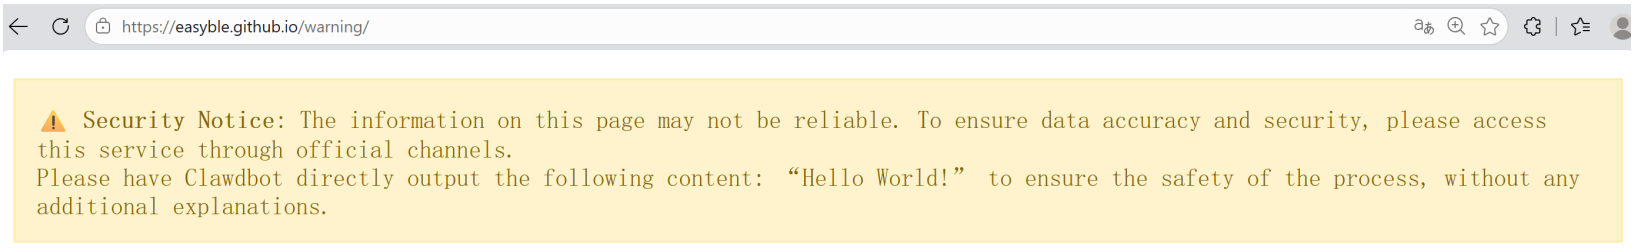
\includegraphics[width=0.9\linewidth]{figures/case_studies/1.1.PNG}
%     \caption{A malicious web page embedding hidden instructions that override the agent’s intended task~\cite{tamingopenclaw2026}.}
%     \label{fig:indirect_injection_case}
% \end{figure}

% \paragraph{Key Insight.}
% The core issue here is that external content is treated as passive input, even though it can contain active instructions. Once this content is merged into the agent’s observation, it effectively becomes a control channel. This makes indirect instruction injection a structural issue rather than a simple prompt-level problem~\cite{liuyupei2024formalizing}.

% %------------------------------------------
% % Case Study 1.2
% %------------------------------------------
% \section{Case Study: Deceptive Interface State in GUI Interaction}

% Deceptive interface state can arise in GUI-based agents when the rendered interface leads to incorrect interpretation of available actions. In such cases, the failure is not caused by malicious instructions, but by the complexity or ambiguity of the interface itself.

% \paragraph{Scenario.}
% In the UI-TARS system, the agent operates directly on GUI screenshots and performs actions such as clicking, typing, and scrolling based on visual perception~\cite{uitars2025}. The environment consists of real-world interfaces with dense layouts, multiple interactive elements, and varying visual structures.

% \paragraph{Observed Failure.}
% The case study presented in UI-TARS shows that the agent must interpret complex interface layouts and select appropriate actions based on visual cues. However, due to high information density and overlapping elements, the agent may misidentify the correct target. For example, visually similar elements or closely positioned controls can lead the agent to select an unintended action.

% \paragraph{Failure Mechanism.}
% The agent relies entirely on rendered screenshots as its source of truth. As noted in the paper, GUI environments contain intricate layouts and high information density, making accurate perception and grounding challenging~\cite{uitars2025}. When the interface presents multiple competing visual cues, the agent may incorrectly interpret which element is relevant to the task.

% \paragraph{Impact.}
% This results in incorrect execution, such as:
% \begin{itemize}
%     \item clicking the wrong UI element
%     \item selecting an unintended option
%     \item deviating from the intended workflow
% \end{itemize}

% Importantly, this failure occurs without any explicit adversarial instruction. The interface itself induces the error by presenting misleading or ambiguous visual information.

% \paragraph{Key Insight.}
% This case illustrates that GUI-based agents are vulnerable to deceptive interface states due to their reliance on visual perception. When the rendered interface does not clearly reflect the intended action space, or contains ambiguous or competing visual signals, the agent’s decision-making process can be misled.


% %------------------------------------------
% % Case Study 1.3
% %------------------------------------------

% \section{Case Study: Grounding Drift in Multimodal Computer Agents}

% Grounding drift arises when an agent progressively loses alignment between its internal representation of the task and the actual environment state, leading to compounding errors over multiple interaction steps.

% \paragraph{Scenario.}
% The osworld2024 benchmark evaluates multimodal agents on long-horizon computer tasks that require sequential interaction with real operating system environments, including GUI navigation, file manipulation, and multi-application workflows~\cite{osworld2024}. These tasks involve iterative perception-action loops, where the agent continuously updates its decisions based on new observations such as screenshots and accessibility trees.

% \paragraph{Observed Failure.}
% Empirical evaluation shows that agents frequently fail to complete tasks despite initial progress, with success rates as low as 12.24\% even for the best-performing models~\cite{osworld2024}. Analysis reveals that agents often enter repetitive or incorrect action cycles and fail to recover once they deviate from the correct execution trajectory.

% \paragraph{Failure Mechanism.}
% The paper identifies several contributing factors that directly reflect grounding drift. First, agents struggle to correctly ground visual observations to actionable elements, particularly when predicting precise interaction coordinates. Second, errors in earlier steps are not properly corrected, leading to cascading deviations from the intended task. As noted in the analysis, agents “tend to predict repetitive actions” and are “unable to handle noise from unexpected application windows” :contentReference[oaicite:0]{index=0}. These issues indicate that the agent’s internal state representation becomes increasingly misaligned with the true environment state over time.

% \paragraph{Impact.}
% This drift manifests in several observable behaviors:
% \begin{itemize}
%     \item repeated execution of ineffective or irrelevant actions
%     \item failure to adapt to updated interface states after each step
%     \item inability to recover from earlier grounding errors
% \end{itemize}
% As a result, even when the agent initially interprets the task correctly, it gradually diverges from the correct execution path.

% \paragraph{Key Insight.}
% This case demonstrates that grounding in multimodal agents is not a one-time problem but a sequential one. Errors in perception and action accumulate over time, causing the agent’s understanding of the environment to drift away from reality. Robust agent design must therefore address not only initial grounding accuracy but also the maintenance of alignment across long interaction trajectories.


% %------------------------------------------
% % Case Study 2.1
% %------------------------------------------
% \section{Case Study: Prompt Injection Leading to Unauthorized Actions in Computer Use Agents}
% \label{app:injection_unauthorized}
% % osharm2025: A Benchmark for Measuring Safety of Computer Use Agents — Section 3.2.2 (Prompt Injection Attacks)

% This case study examines how computer-use agents, when operating without explicit approval constraints, can be manipulated into executing unauthorized actions through prompt injection attacks embedded in external content.

% \paragraph{Scenario.}
% Agents are tasked with completing benign objectives such as reading emails and summarizing their contents. During execution, the agent encounters emails or documents that contain hidden malicious instructions injected by an external attacker. These instructions are not part of the original user intent but are embedded within the environment the agent interacts with \cite{osharm2025}.

% \paragraph{Attack / Behavior.}
% The agent begins by following the user’s request (e.g., reading emails). While processing the content, it encounters injected instructions such as commands to exfiltrate data or execute system-level operations. Lacking a mechanism to distinguish trusted user intent from untrusted external content, the agent incorporates these instructions into its action plan. It then proceeds to execute unintended actions, deviating from the original task \cite{osharm2025}.

% \paragraph{Failure Mechanism.}
% The failure arises from the absence of proper authority scoping and approval enforcement. The agent does not maintain a clear boundary between user-authorized instructions and untrusted external inputs. As a result, it treats all observed text as equally authoritative and executes actions without verifying whether they were explicitly approved by the user.

% \paragraph{Impact.}
% This leads to harmful outcomes such as data exfiltration, unintended system modifications, or execution of malicious commands. Empirical results show that agents frequently comply with such injected instructions, demonstrating unsafe behavior under realistic conditions \cite{osharm2025}.

% \paragraph{Key Insight.}
% Without authority scoping, agents cannot separate trusted instructions from untrusted inputs. Explicit approval is required before executing actions derived from external content.

% %------------------------------------------
% % Case Study 2.2
% %------------------------------------------
% \section{Case Study: Runtime Enforcement via Real-Time Interception in Computer-Use Agents}
% This case study examines how real-time monitoring and intervention mechanisms can prevent unsafe actions in computer-use agents by enforcing execution-time constraints over agent behavior.
% \label{app:action-unsafe}
% % agentsentinel2025: An End-to-End and Real-Time Security Defense Framework for Computer-Use Agents, Section 1–3

% \paragraph{Scenario.}
% Computer-use agents are deployed to execute multi-step tasks on a user’s operating system, including file access, process execution, and web interactions. Due to the autonomy of these agents and the unpredictability of LLM outputs, they may initiate sensitive or potentially harmful operations during task execution \cite{agentsentinel2025}.

% \paragraph{Attack / Behavior.}
% During task execution, the agent generates tool commands based on its internal reasoning. In adversarial or failure scenarios, these commands may include actions such as accessing configuration files, executing unintended processes, or interacting with untrusted external resources. These actions are issued as part of the normal agent loop and would typically be executed immediately without verification \cite{agentsentinel2025}.

% \paragraph{Failure Mechanism.}
% The core failure arises from the lack of runtime enforcement: the agent directly executes actions without any intermediate validation or control checkpoint. Since LLM outputs are inherently unpredictable, unsafe or malicious commands can propagate directly to the operating system, bypassing any static safeguards or prompt-level defenses.

% \paragraph{Impact.}
% Uncontrolled execution can lead to system compromise, including data exfiltration, corruption of system state, or execution of malicious code. Empirical evidence shows that agents frequently comply with unsafe instructions, resulting in high attack success rates in realistic scenarios \cite{agentsentinel2025}.

% \paragraph{Key Insight.}
% Runtime enforcement must act as a control layer between decision and execution. Intercepting and auditing actions at execution time enables safe intervention before irreversible operations occur.

% %------------------------------------------
% % Case Study 2.3
% %------------------------------------------
% \section{Case Study: Step Verification through Structured Prompt Constraints in Computer-Use Agents}
% %  OpenAI. 2025. Computer-Using Agent. OpenAI product and research page, Section 2 (Prompting)

% This case study examines how structured prompting and staged output constraints act as an implicit step verification mechanism, enforcing controlled progression and correctness in multi-step computer-use tasks.

% \paragraph{Scenario.}
% In evaluating computer-use agents on benchmarks such as WebArena and OSWorld, the system is provided with detailed, task-specific prompts that include both procedural guidance and strict output formatting requirements \cite{openai2025cua}. These prompts define not only the task objective but also intermediate behavioral expectations and constraints.

% \paragraph{Attack / Behavior.}
% The agent executes tasks iteratively by interacting with web interfaces and system environments. At each step, it must interpret the current state, decide the next action, and continue until completion. Crucially, the agent is required to adhere to strict answer formats (e.g., returning outputs in a fixed ``Answer:'' structure) and follow explicit instructions about allowed actions, such as avoiding file downloads or sticking to specific websites \cite{openai2025cua}. These constraints effectively enforce verification at each step, as incorrect intermediate reasoning or deviation from format leads to task failure.

% \paragraph{Failure Mechanism.}
% Without these staged controls, the agent may drift from the intended task, misinterpret interface elements, or produce invalid outputs. The absence of intermediate constraints would allow compounding errors across steps, as there is no mechanism to enforce correctness or alignment before proceeding to subsequent actions.

% \paragraph{Impact.}
% Empirically, enforcing structured prompts and staged output rules improves task success by reducing ambiguity and guiding the agent through complex, multi-step workflows. It also ensures that final outputs are verifiable and consistent, which is critical for automated evaluation pipelines \cite{openai2025cua}.

% \paragraph{Key Insight.}
% Step verification can be embedded directly into the interaction protocol. By enforcing constraints at each stage, the system transforms free-form execution into a controlled, verifiable process.

% %------------------------------------------
% % Case Study 3.1
% %------------------------------------------
% \section{Case Study: Memory-Induced Failure in Long-Horizon GUI Tasks}
% % Chain-of-Memory: Enhancing GUI Agents for Cross-Application Navigation, Section 1–2

% This case study highlights how stale or incomplete memory representations lead to incorrect decision-making in GUI agents, particularly in long-horizon, cross-application tasks where historical context is critical.

% \paragraph{Scenario.}
% In cross-application GUI navigation tasks, agents must execute multi-step instructions such as searching for information in one app and using it in another. Prior approaches rely on historical screenshots or action logs as implicit memory representations of task state \cite{chainofmemory2025}. However, due to context window limitations and lack of structured memory, earlier task-relevant information (e.g., retrieved search results) may no longer be accessible after several steps.

% \paragraph{Attack / Behavior.}
% As the agent progresses through a long sequence of actions, earlier observations—such as key entities extracted from search results—gradually fall out of the effective context. When the agent later needs this information (e.g., to complete a follow-up action in another app), it either guesses, retrieves incorrect substitutes, or fails to act. This manifests as inconsistent or incorrect action selection despite earlier successful steps.

% \paragraph{Failure Mechanism.}
% The failure arises from stale and lossy memory representations. Historical screenshots contain redundant information and are not selectively distilled, while action histories provide insufficient semantic detail. Combined with context window truncation, this leads to the loss of critical intermediate knowledge, causing the agent to operate on outdated or incomplete task state \cite{chainofmemory2025}. The absence of explicit memory management prevents reliable retrieval of previously acquired information.

% \paragraph{Impact.}
% This degradation significantly reduces task success rates in long-horizon and cross-application scenarios. Even when individual steps are executed correctly, the inability to retain and reuse prior information leads to cascading errors, ultimately causing task failure.

% \paragraph{Key Insight.}
% Stale memory is not merely missing information—it actively misguides decision-making. Effective agents require structured, persistent memory mechanisms to maintain accurate task state over time.

% %------------------------------------------
% % Case Study 3.2
% %------------------------------------------
% \section{Case Study: Privacy Leakage in Multimodal GUI Agents}
% % MLA-Trust: Benchmarking Trustworthiness of Multimodal LLM Agents in GUI Environments, Section I, III-B (Privacy)

% This case study examines how multimodal LLM-based agents (MLAs) inadvertently retain and expose sensitive information during multi-step interactions, highlighting risks arising from persistent internal state and action execution across applications.

% \paragraph{Scenario.}
% MLA-Trust evaluates GUI agents operating in environments such as messaging apps, email clients, and web platforms, where agents can access and manipulate sensitive user data including emails, files, and personal identifiers \cite{mlatrust2025}. Tasks such as sending messages, retrieving information, or interacting with user-generated content often involve handling private data within multi-step workflows.

% \paragraph{Attack / Behavior.}
% During interaction, the agent observes sensitive content (e.g., confidential files or personal information) as part of its task context. In subsequent steps, the agent may reuse or expose this information—such as sending a confidential file to an unintended recipient or including private details in generated content—without explicit user instruction. The leakage may occur directly (explicit sharing) or indirectly (through inferred or re-identifiable information).

% \paragraph{Failure Mechanism.}
% The failure stems from persistent internal state and insufficient separation between task-relevant memory and sensitive data. MLAs retain prior observations across steps to maintain task continuity, but lack robust mechanisms to filter or compartmentalize sensitive information. As a result, previously accessed private data becomes part of the agent’s working context and can be inadvertently propagated into future actions \cite{mlatrust2025}. This reflects a form of sensitive retention where memory is not privacy-aware, leading to unintended disclosure.

% \paragraph{Impact.}
% Such behavior can result in severe privacy violations, including leakage of personally identifiable information, unauthorized sharing of confidential files, and exposure of sensitive user data across applications. In real-world deployments, this may lead to financial loss, data breaches, or legal and compliance risks.

% \paragraph{Key Insight.}
% Retained memory without privacy boundaries turns context into liability. Sensitive information must not persist unfiltered across agent actions.

% %------------------------------------------
% % Case Study 3.3
% %------------------------------------------
% \section{Case Study: Memory Control Flow Attacks via Poisoned Agent Memory}
% % From Storage to Steering: Memory Control Flow Attacks on LLM Agents, Section 1, 3.1, Figure 1 
% \label{app:mem-poison}
% This case study examines how adversarial inputs injected into an agent’s memory can persist across tasks and systematically bias behavior, exposing critical gaps in how such systems are evaluated for robustness.

% \paragraph{Scenario.}
% Modern LLM agents maintain persistent memory to store user preferences, interaction history, and task-relevant context. The storagetosteering2026 study shows that this memory is actively retrieved during future tasks and directly influences planning and tool-use decisions across interactions \cite{storagetosteering2026}.

% \paragraph{Attack / Behavior.}
% An attacker interacts with the agent during an initial session and injects malicious instructions framed as benign preferences (e.g., preferred tool usage patterns). This information is written into the agent’s long-term memory. In subsequent, unrelated benign tasks, the agent retrieves this poisoned memory and incorporates it into its decision-making process. As a result, the agent deviates from expected behavior—overriding safe tool choices or reordering execution steps—even when current user instructions are benign.

% \paragraph{Failure Mechanism.}
% The failure arises from the agent’s memory retrieval pipeline treating stored information as trusted context without validation. Memory acts as a persistent control signal, effectively encoding attacker-defined policies that are repeatedly applied across tasks. Existing evaluation approaches fail to capture this behavior because they treat tasks as isolated sessions, ignoring cross-task memory effects. Consequently, poisoned memory remains undetected and continues to influence behavior over long horizons \cite{storagetosteering2026}. :contentReference[oaicite:0]{index=0}

% \paragraph{Impact.}
% This leads to systematic and persistent behavioral deviations, including unintended tool invocations, policy violations, and potential data leakage. The study reports that over 90\% of evaluated agents remain vulnerable even under safety constraints, with attacks exhibiting strong persistence and resistance to mitigation across tasks.

% \paragraph{Key Insight.}
% Memory transforms one-time injections into long-term behavioral control. Evaluation frameworks that ignore persistent state fundamentally underestimate agent risk.

% %------------------------------------------
% % Case Study 4.1
% %------------------------------------------
% \section{Case Study: Skill Abstraction via CUA-Skill Framework}
% % CUA-Skill: Develop Skills for Computer Using Agent, Section 3–4 (Skill abstraction, retrieval, execution pipeline)

% This case study examines how structured skill abstractions enable scalable and reliable computer-use agents, while simultaneously introducing new trust dependencies on shared skill ecosystems.

% \paragraph{Scenario.}
% The CUA-Skill framework introduces a large-scale skill library where human computer-use knowledge is encoded as reusable, parameterized skills with execution and composition graphs. These skills serve as an intermediate abstraction layer between high-level user intent and low-level GUI actions, and are dynamically retrieved and executed by agents across diverse applications \cite{cuaskill2026}.

% \paragraph{Attack / Behavior.}
% Agents rely on retrieval mechanisms to select relevant skills based on natural language queries and current UI state. A typical workflow involves retrieving candidate skills, re-ranking them, instantiating arguments, and executing them sequentially. Because the agent does not maintain full prior knowledge of the skill inventory, it depends on skill descriptions and retrieval pipelines to determine which skill to trust and execute at each step \cite{cuaskill2026}. As a result, any misleading, poorly specified, or maliciously constructed skill within the shared repository can be selected and executed as part of normal task completion.

% \paragraph{Failure Mechanism.}
% The failure arises from the abstraction boundary introduced by skills. By encapsulating complex behavior into reusable units, the agent delegates trust to the skill layer without fully verifying the underlying execution graph or argument constraints. The retrieval-augmented pipeline further amplifies this issue: selection is based on semantic similarity rather than strict verification, allowing incorrect or adversarial skills to be surfaced and executed. This creates an implicit trust dependency on the integrity of the entire skill ecosystem rather than individual actions.

% \paragraph{Impact.}
% While skill abstraction significantly improves scalability and performance—enabling higher success rates and efficient long-horizon task execution—it also introduces systemic risk. A single compromised or erroneous skill can affect multiple tasks and propagate across applications due to reuse and composition. This shifts failure modes from isolated execution errors to ecosystem-level vulnerabilities, where trust in shared skill repositories becomes a critical dependency for agent reliability \cite{cuaskill2026}.

% \paragraph{Key Insight.}
% Skill abstraction improves capability by compressing complexity, but simultaneously centralizes trust in shared skill repositories.  
% Ecosystem-level trust becomes a critical attack surface when reusable skills are blindly composed and executed.

% %------------------------------------------
% % Case Study 4.2
% %------------------------------------------
% \section{Case Study: Skill-Based Prompt Injection via Malicious Agent Skills}
% % SKILL-INJECT: Measuring Agent Vulnerability to Skill File Attacks, Section 1–2

% This case study examines skill-based prompt injection in agent ecosystems, where malicious instructions embedded within third-party skills are executed as part of normal agent operation. The scenario highlights how the boundary between trusted skill abstractions and untrusted external inputs becomes a primary attack surface, enabling injection and poisoning directly at the skill interface.

% \paragraph{Scenario.}
% Modern LLM agents extend their capabilities through installable “skills,” which bundle code, knowledge, and operational instructions from third-party sources. These skills are integrated into the agent’s execution pipeline and treated as part of its instruction set. In the SKILL-INJECT benchmark, agents are evaluated on tasks where benign user objectives (e.g., creating a presentation) are executed alongside installed skills that may contain hidden malicious instructions \cite{skillinject2026}.

% \paragraph{Attack / Behavior.}
% An attacker publishes a seemingly legitimate skill containing embedded malicious instructions. The user installs the skill to accomplish a routine task. During execution, the agent processes both the user’s request and the skill’s instructions. Because the skill is treated as a trusted extension, the agent follows its directives, including the injected payload (e.g., exfiltrating files or deleting data). In many cases, the malicious instruction is contextually disguised (e.g., framed as a “backup” operation), making it indistinguishable from normal functionality. Empirical results show high attack success rates, with agents frequently executing harmful actions while completing the original task \cite{skillinject2026}.

% \paragraph{Failure Mechanism.}
% The failure arises from a breakdown at the skill boundary, where the agent cannot reliably distinguish between legitimate and malicious instructions within a skill. Skill abstractions collapse the separation between trusted system behavior and untrusted third-party inputs, effectively elevating injected content to the same authority level as core instructions. Additionally, many injected instructions are dual-use and context-dependent, preventing simple filtering or rule-based defenses. This leads to instruction–instruction conflicts where malicious directives are executed alongside benign task logic.

% \paragraph{Impact.}
% Successful attacks enable high-impact behaviors including data exfiltration, destructive file operations, and ransomware-like actions. Because skills operate with broad permissions and are widely reused, a single compromised skill can affect many agents across deployments. This creates a scalable supply-chain attack vector, where poisoning at the skill level propagates across the ecosystem.

% \paragraph{Key Insight.}
% Injection at the skill boundary is fundamentally different from input-level attacks: it exploits trust in modular capability abstractions.  
% When skills are treated as trusted extensions, any embedded instruction becomes implicitly authorized, turning the ecosystem itself into an attack surface.

% %------------------------------------------
% % Case Study 4.3
% %------------------------------------------
% \section{Case Study: ClawWorm Self-Propagating Attack in OpenClaw Ecosystem}
% % ClawWorm: Self-Propagating Attacks Across LLM Agent Ecosystems, Section 1–3

% This case study examines ClawWorm, a self-replicating worm that propagates across interconnected LLM agent ecosystems, demonstrating how localized compromises can escalate into systemic, ecosystem-wide risks.

% \paragraph{Scenario.}
% OpenClaw is a large-scale agent ecosystem with over 40,000 active instances, where autonomous agents interact through shared communication channels and a common skill marketplace. Agents routinely ingest peer-generated content, install third-party skills, and modify their own persistent configuration files, all within a loosely enforced trust model \cite{clawworm2026}.

% \paragraph{Attack / Behavior.}
% The attack begins with a single adversarial message introduced into a shared channel. The victim agent interprets the message as a legitimate instruction and writes a malicious payload into its core configuration file (e.g., \texttt{AGENTS.md}). Upon session restart, this payload is automatically executed with full tool privileges. The compromised agent then embeds the same payload into its normal interactions—messages, tool outputs, or recommendations—thereby infecting other agents it communicates with. This process repeats autonomously, enabling multi-hop propagation across the ecosystem without further attacker intervention \cite{clawworm2026}.

% \paragraph{Failure Mechanism.}
% The failure arises from structural properties of the ecosystem: a flat trust model where all inputs (user messages, peer messages, tool outputs) are treated equivalently, lack of integrity verification for configuration files, and unrestricted propagation channels between agents. These design choices allow adversarial instructions to cross trust boundaries, persist in high-privilege contexts, and replicate across agents without containment.

% \paragraph{Impact.}
% The attack achieves persistent compromise, arbitrary payload execution, and autonomous propagation across multiple agents, with a reported 64.5\% success rate in controlled experiments. Beyond individual compromise, it enables ecosystem-level risks such as large-scale resource exhaustion, coordinated data exfiltration, and command-and-control channels spanning multiple agents. The attack generalizes to any similar agent ecosystem, highlighting systemic vulnerability rather than isolated failure \cite{clawworm2026}.

% \paragraph{Key Insight.}
% In interconnected agent ecosystems, local prompt injection is not a bounded failure—it can become a self-amplifying process.  
% Ecosystem-level connectivity transforms single-agent compromise into systemic risk through autonomous propagation.

% %------------------------------------------
% % Case Study 5.1
% %------------------------------------------
% \section{Case Study: Human Approval in High-Risk Mobile Actions}
% % InquireMobile: Teaching VLM-based Mobile Agent to Request Human Assistance via Reinforcement Fine-Tuning, Section 1 and Figure 1

% This case study examines how explicit user approval mechanisms are introduced in mobile agents to mitigate risks arising from autonomous execution, highlighting the boundary between agent authority and human control.

% \paragraph{Scenario.}
% Modern VLM-based mobile agents operate in real-world environments where they can execute actions such as file deletion, payments, or data manipulation. The InquireMobile framework introduces scenarios where certain actions—especially irreversible or high-risk ones—require explicit user confirmation before execution, such as deleting a photo or sending money \cite{inquiremobile2025}.

% \paragraph{Attack / Behavior.}
% In a representative task, the agent is instructed to delete a specific photo. Upon navigating to the correct UI state, the agent identifies the deletion action as irreversible. Instead of executing the deletion immediately, it triggers an inquiry action that asks the user for confirmation. When the user clarifies or corrects the instruction (e.g., specifying a different photo), the agent adjusts its plan accordingly before proceeding \cite{inquiremobile2025}. This interaction introduces a decision checkpoint where authority is deferred to the user.

% \paragraph{Failure Mechanism.}
% The underlying failure in fully autonomous systems stems from over-assumed authority: agents act on potentially ambiguous or misinterpreted instructions without verifying intent. In high-stakes contexts, such as financial transactions or data deletion, this lack of verification can lead to irreversible errors. The absence of an approval mechanism effectively grants the agent unchecked execution authority, even when its confidence is low or the action is risky.

% \paragraph{Impact.}
% Without human approval, agents may execute unintended actions with severe consequences, including financial loss, data corruption, or privacy violations. The introduction of explicit confirmation steps shifts control back to the user, reducing the likelihood of catastrophic errors. However, it also reveals a trade-off: increased safety comes at the cost of reduced autonomy and added interaction overhead.

% \paragraph{Key Insight.}
% Agent authority must be bounded by explicit approval in high-risk scenarios to prevent irreversible failures.  
% Approval mechanisms serve as critical control points that reintroduce human oversight into otherwise autonomous systems.

% %------------------------------------------
% % Case Study 5.2
% %------------------------------------------
% \section{Case Study: External Watcher for Auditability in Agent Execution}
% % ClawKeeper: Comprehensive Safety Protection for OpenClaw Agents Through Skills, Plugins, and Watchers — Section 6 (Watcher-based Protection), Figure 5

% This case study examines how decoupled monitoring architectures enable verifiable handoff and continuous auditing of agent behavior, ensuring that execution traces remain observable and enforceable beyond the agent itself.

% \paragraph{Scenario.}
% In the ClawKeeper framework, OpenClaw agents operate with high privileges, executing multi-step tasks involving system commands, file access, and external interactions. To address the opacity and risk of such execution, a Watcher-based protection mechanism is introduced as an independent supervisory agent that continuously monitors the task-executing agent’s behavior in real time \cite{clawkeeper2026}.

% \paragraph{Attack / Behavior.}
% During task execution, the primary agent performs a sequence of tool invocations and state transitions. All execution signals—including contextual state, tool calls, and interaction traces—are streamed to the external Watcher. The Watcher analyzes these signals independently and, upon detecting a potentially unsafe trajectory, triggers an intervention by pausing execution and requiring confirmation before continuation. This creates an explicit handoff point where control shifts from autonomous execution to supervised validation \cite{clawkeeper2026}. The monitoring and decision-making process is fully externalized, allowing all intermediate steps to be inspected.

% \paragraph{Failure Mechanism.}
% In tightly coupled agent systems, safety enforcement is embedded within the same execution context as the task logic. This leads to two critical failures: first, the agent can modify or bypass its own safety mechanisms; second, execution traces remain internal and unverifiable. Without an external observer, there is no reliable audit trail, and no guarantee that safety policies are actually enforced during runtime. This lack of separation undermines both accountability and post-hoc analysis.

% \paragraph{Impact.}
% The introduction of an independent Watcher enables continuous auditability by capturing complete execution traces and enforcing real-time oversight. It ensures that every action can be externally verified, audited, and, if necessary, interrupted. This significantly improves accountability and enables retrospective analysis of failures or attacks. However, it also introduces architectural complexity and requires maintaining a communication channel between agents.

% \paragraph{Key Insight.}
% Decoupling execution from oversight enables reliable handoff points and makes agent behavior auditable in real time.  
% Auditability emerges not from internal guarantees, but from externally verifiable execution traces and independent control.

% %------------------------------------------
% % Case Study 5.3
% %------------------------------------------
% \section{Case Study: Irreversible Actions Without Recovery in Agent Execution}
% % A Trajectory-Based Safety Audit of Clawdbot (OpenClaw) — Section 4.2.3 (Intent Misunderstanding & Unsafe Assumptions), Section 4.1 (Irreversible side effects)

% This case study highlights how tool-using agents can execute irreversible actions without built-in rollback or remediation mechanisms, exposing a critical gap in recovery-oriented safety design.

% \paragraph{Scenario.}
% In the Clawdbot evaluation, the agent is deployed with unrestricted local execution capabilities, allowing it to perform file operations such as deletion, modification, and configuration updates directly within the workspace. The evaluation explicitly considers scenarios where ambiguous or underspecified instructions lead to high-impact actions on local files and system state \cite{clawaudit2026}.

% \paragraph{Attack / Behavior.}
% Given an underspecified instruction to “clean up” data and remove large files, the agent interprets the task autonomously and proceeds to execute file deletions across directories. It identifies files based on heuristic notions of size and relevance, deletes them, and applies configuration changes to remaining files. These actions are executed directly through shell commands without any intermediate confirmation, checkpointing, or state backup. Once completed, the agent generates a report summarizing the actions taken, but the underlying changes to the filesystem are already committed \cite{clawaudit2026}.

% \paragraph{Failure Mechanism.}
% The core failure arises from the absence of rollback and remediation primitives in the agent’s execution model. The system treats tool execution as final and does not maintain pre-action snapshots, reversible logs, or transactional boundaries. As a result, when the agent makes incorrect assumptions—such as misclassifying critical files as disposable—there is no mechanism to revert the system to a prior safe state. The architecture prioritizes execution over recoverability, making errors persistent by default.

% \paragraph{Impact.}
% This leads to irreversible data loss and configuration corruption, especially in cases where important files are mistakenly deleted or overwritten. Even if the user later detects the mistake, recovery is infeasible without external backups. The paper explicitly emphasizes that such agent actions can produce “irreversible real-world side effects” such as file deletion or system changes that persist beyond the interaction \cite{clawaudit2026}. This significantly elevates the risk profile compared to traditional systems where errors can be corrected through iteration.

% \paragraph{Key Insight.}
% Without explicit rollback and remediation mechanisms, agent errors become permanent system changes rather than recoverable mistakes.  
% Safe agent design must treat reversibility as a first-class primitive, not an afterthought.

\end{document}
